\documentclass[12pt]{extarticle}
\usepackage[paperwidth=15in,paperheight=7.2in]{geometry}
\usepackage{amsmath}
\usepackage{hyperref}
\usepackage{multirow}
\usepackage{pdfpages}
\usepackage[utf8]{inputenc}
\title{Kaon mixing: chiral and continuum extrapolations}
\author{R Mukherjee}
\date{\today}
\begin{document}
\maketitle
\tableofcontents
\clearpage
\begin{figure}
\centering
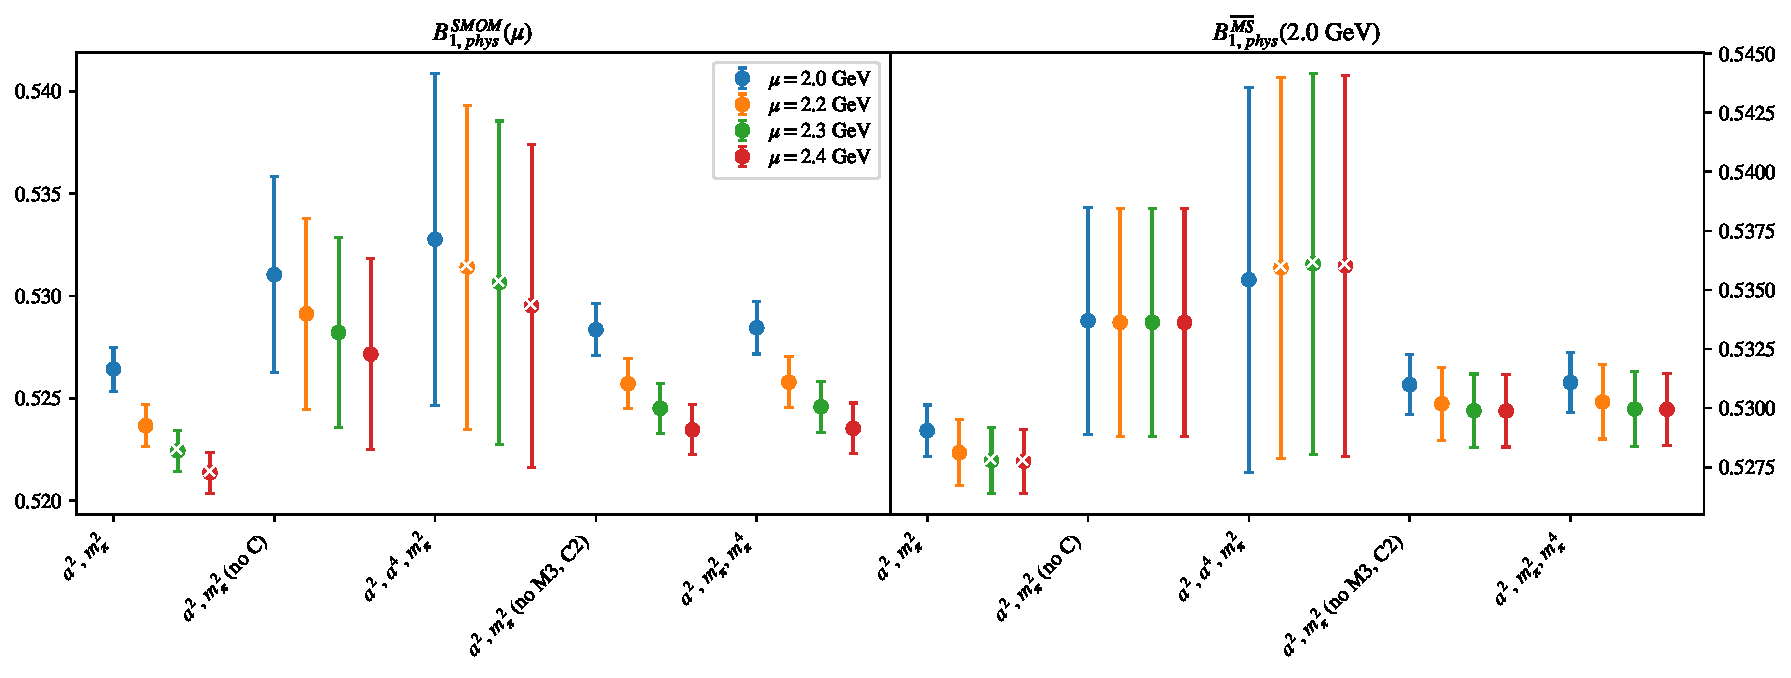
\includegraphics[page=1, width=1.1\textwidth]{VVpAA/SUSY_F/fit_summary.pdf}
\caption{$B_{1}$\\(left) $B_{phys}$ in RI/SMOM scheme from fit variations (fits with $p$-value $<0.05$ marked with ``$\times$"). \\(right) $B_{phys}$ in $\overline{MS}$ computed using $B^{\overline{MS}} = R^{\overline{MS}\leftarrow SMOM}(2.0)\sigma_{npt}(2.0,\mu) B^{SMOM}(\mu)$.}
\end{figure}
\clearpage
\begin{figure}
\centering
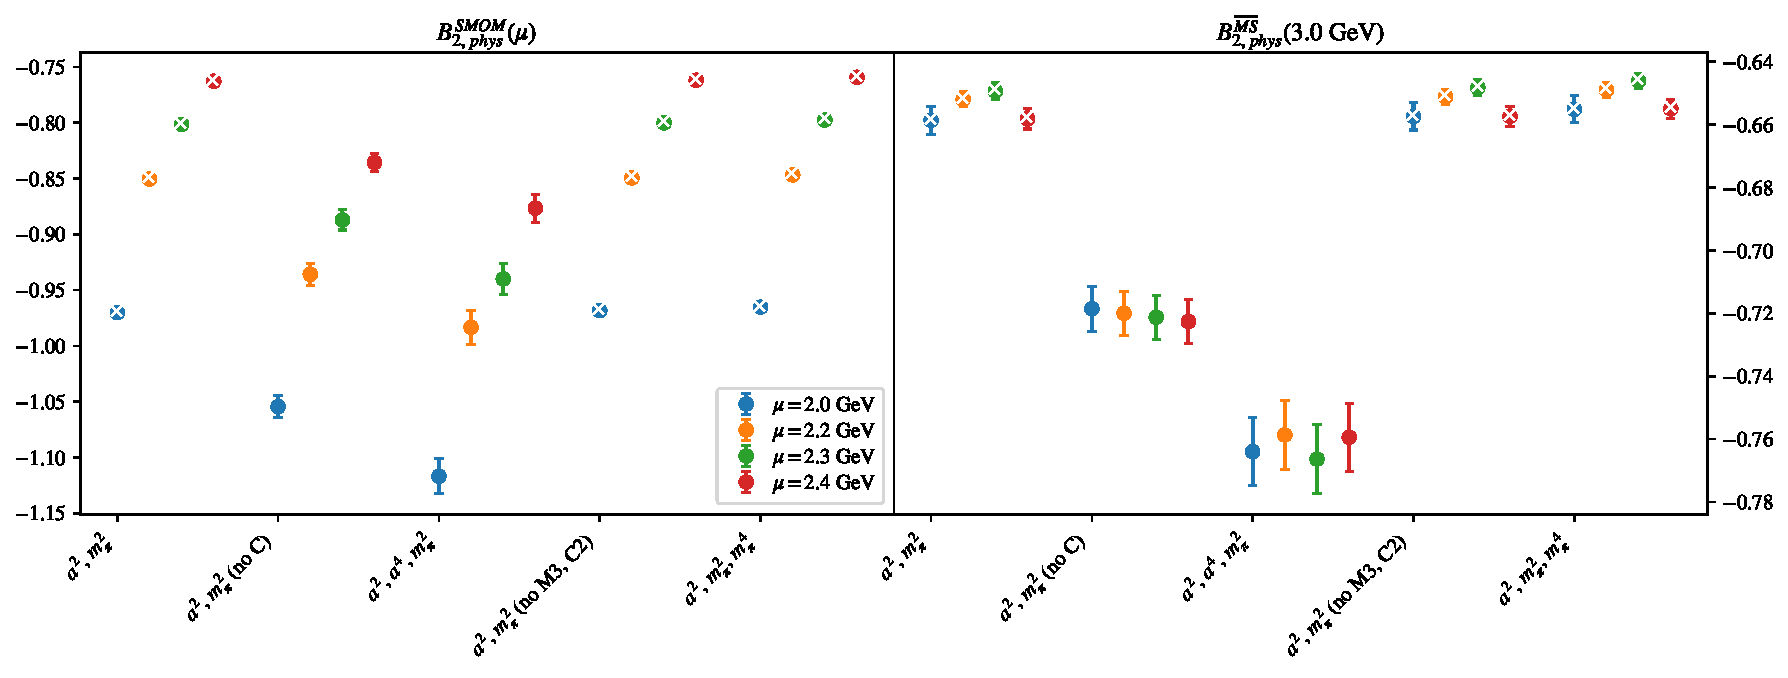
\includegraphics[page=1, width=1.1\textwidth]{VVmAA/SUSY_F/fit_summary.pdf}
\caption{$B_{2}$\\(left) $B_{phys}$ in RI/SMOM scheme from fit variations (fits with $p$-value $<0.05$ marked with ``$\times$"). \\(right) $B_{phys}$ in $\overline{MS}$ computed using $B^{\overline{MS}} = R^{\overline{MS}\leftarrow SMOM}(3.0)\sigma_{npt}(3.0,\mu) B^{SMOM}(\mu)$.}
\end{figure}
\clearpage
\begin{figure}
\centering
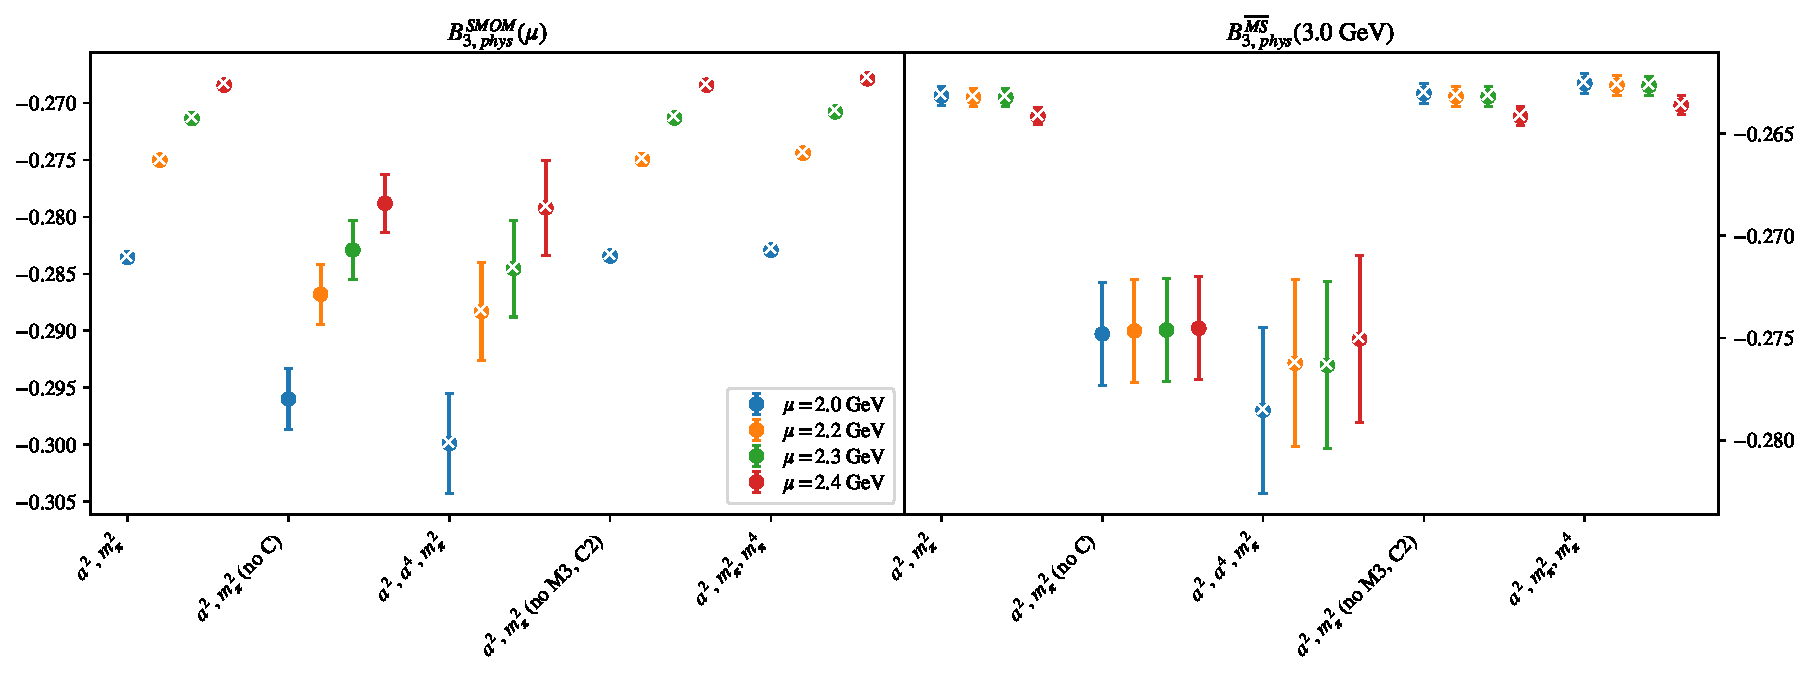
\includegraphics[page=1, width=1.1\textwidth]{SSmPP/SUSY_F/fit_summary.pdf}
\caption{$B_{3}$\\(left) $B_{phys}$ in RI/SMOM scheme from fit variations (fits with $p$-value $<0.05$ marked with ``$\times$"). \\(right) $B_{phys}$ in $\overline{MS}$ computed using $B^{\overline{MS}} = R^{\overline{MS}\leftarrow SMOM}(3.0)\sigma_{npt}(3.0,\mu) B^{SMOM}(\mu)$.}
\end{figure}
\clearpage
\begin{figure}
\centering
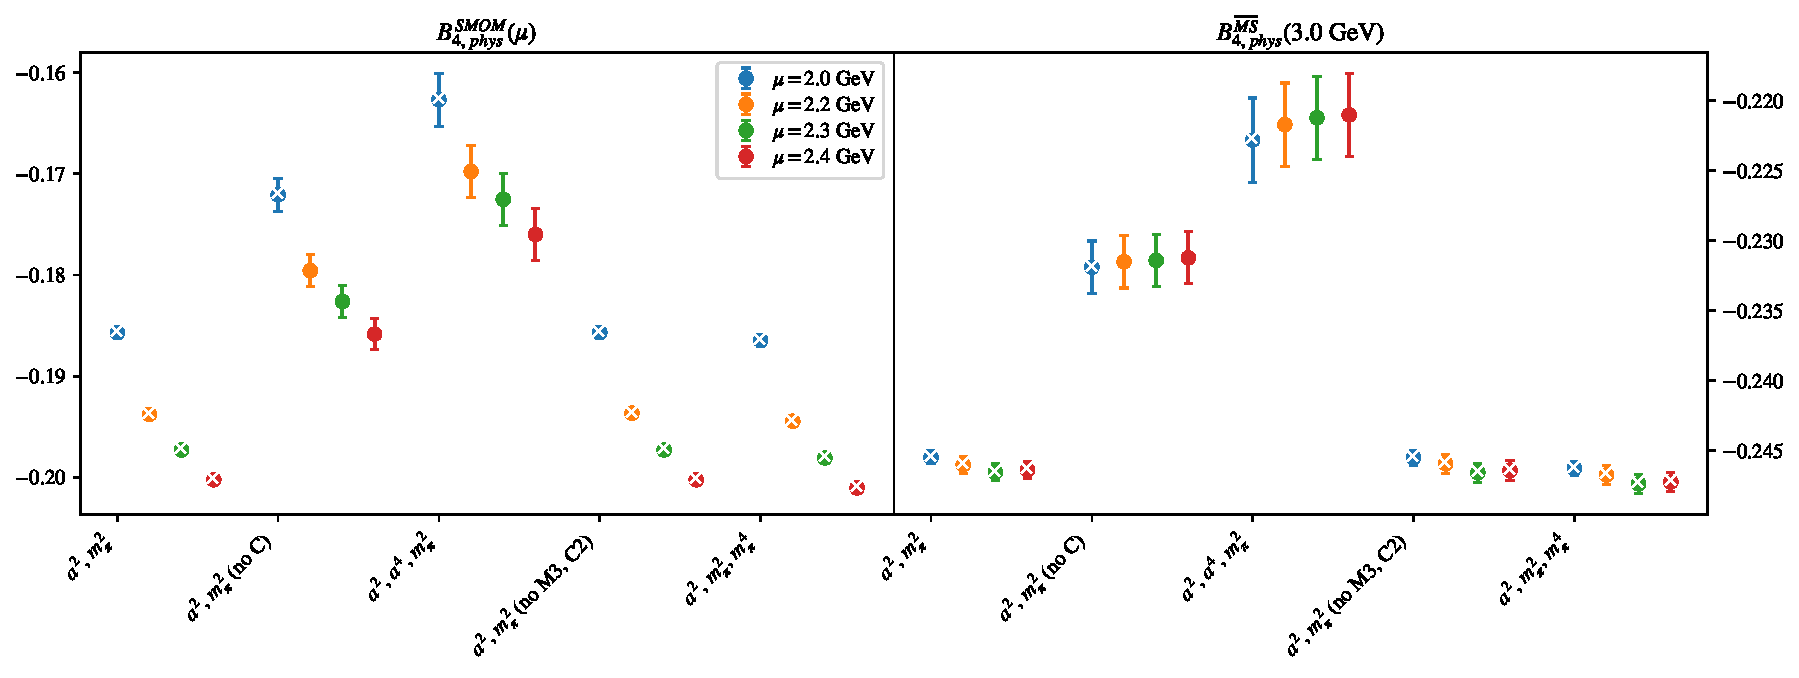
\includegraphics[page=1, width=1.1\textwidth]{SSpPP/SUSY_F/fit_summary.pdf}
\caption{$B_{4}$\\(left) $B_{phys}$ in RI/SMOM scheme from fit variations (fits with $p$-value $<0.05$ marked with ``$\times$"). \\(right) $B_{phys}$ in $\overline{MS}$ computed using $B^{\overline{MS}} = R^{\overline{MS}\leftarrow SMOM}(3.0)\sigma_{npt}(3.0,\mu) B^{SMOM}(\mu)$.}
\end{figure}
\clearpage
\begin{figure}
\centering
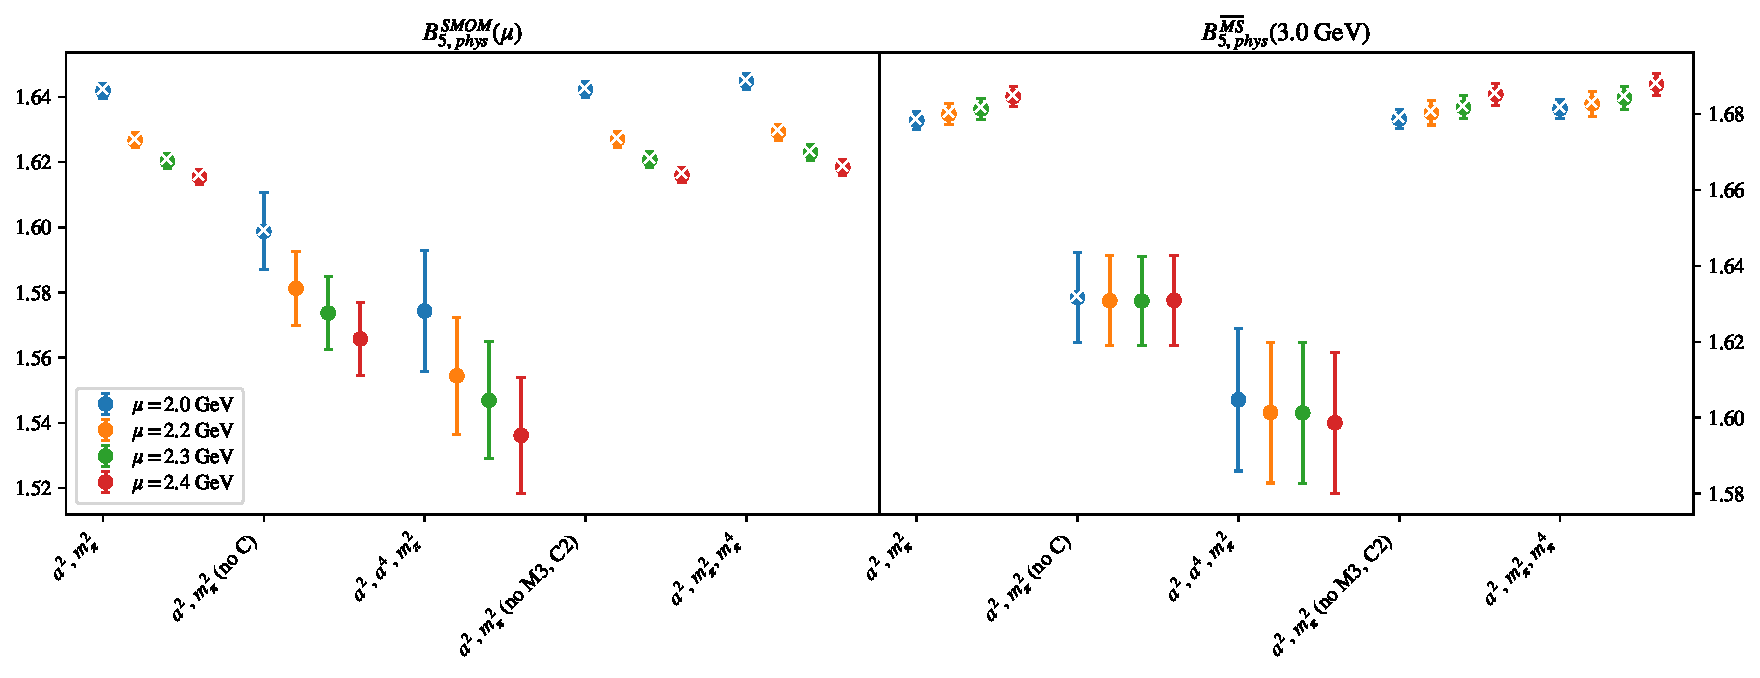
\includegraphics[page=1, width=1.1\textwidth]{TT/SUSY_F/fit_summary.pdf}
\caption{$B_{5}$\\(left) $B_{phys}$ in RI/SMOM scheme from fit variations (fits with $p$-value $<0.05$ marked with ``$\times$"). \\(right) $B_{phys}$ in $\overline{MS}$ computed using $B^{\overline{MS}} = R^{\overline{MS}\leftarrow SMOM}(3.0)\sigma_{npt}(3.0,\mu) B^{SMOM}(\mu)$.}
\end{figure}
\clearpage
\section{$B_1$}
\begin{table}[h!]
\begin{center}
\begin{tabular}{|c|c|c|c|c|c|}
\hline
$\mu$ (GeV) & $a^2$, $m_\pi^2$& $a^2$, $m_\pi^2$ (no C)& $a^2$, $a^4$, $m_\pi^2$& $a^2$, $m_\pi^2$ (no M3, C2)& $a^2$, $m_\pi^2$, $m_\pi^4$\\
\hline
2.0& \hyperlink{VVpAA/SUSY_F/a2m2_20.pdf.1}{\textbf{0.5264(10)}: 1.858 (0.098)} & \hyperlink{VVpAA/SUSY_F/a2m2noC_20.pdf.1}{\textbf{0.5310(47)}: 0.876 (0.417)} & \hyperlink{VVpAA/SUSY_F/a2a4m2_20.pdf.1}{\textbf{0.5327(81)}: 2.173 (0.069)} & \hyperlink{VVpAA/SUSY_F/a2m2mcut_20.pdf.1}{\textbf{0.5283(12)}: 0.248 (0.863)} & \hyperlink{VVpAA/SUSY_F/a2m2m4_20.pdf.1}{\textbf{0.5284(12)}: 0.661 (0.619)}\\
2.2& \hyperlink{VVpAA/SUSY_F/a2m2_22.pdf.1}{\textbf{0.5236(10)}: 2.214 (0.05)} & \hyperlink{VVpAA/SUSY_F/a2m2noC_22.pdf.1}{\textbf{0.5291(46)}: 1.143 (0.319)} & \hyperlink{VVpAA/SUSY_F/a2a4m2_22.pdf.1}{\textbf{0.5314(79)}: 2.525 (0.039)} & \hyperlink{VVpAA/SUSY_F/a2m2mcut_22.pdf.1}{\textbf{0.5257(12)}: 0.36 (0.782)} & \hyperlink{VVpAA/SUSY_F/a2m2m4_22.pdf.1}{\textbf{0.5257(12)}: 0.923 (0.449)}\\
2.3& \hyperlink{VVpAA/SUSY_F/a2m2_23.pdf.1}{\textbf{0.5224(10)}: 2.304 (0.042)} & \hyperlink{VVpAA/SUSY_F/a2m2noC_23.pdf.1}{\textbf{0.5282(46)}: 1.197 (0.302)} & \hyperlink{VVpAA/SUSY_F/a2a4m2_23.pdf.1}{\textbf{0.5306(78)}: 2.605 (0.034)} & \hyperlink{VVpAA/SUSY_F/a2m2mcut_23.pdf.1}{\textbf{0.5245(12)}: 0.411 (0.745)} & \hyperlink{VVpAA/SUSY_F/a2m2m4_23.pdf.1}{\textbf{0.5245(12)}: 0.993 (0.41)}\\
2.4& \hyperlink{VVpAA/SUSY_F/a2m2_24.pdf.1}{\textbf{0.5213(10)}: 2.348 (0.039)} & \hyperlink{VVpAA/SUSY_F/a2m2noC_24.pdf.1}{\textbf{0.5271(46)}: 1.223 (0.294)} & \hyperlink{VVpAA/SUSY_F/a2a4m2_24.pdf.1}{\textbf{0.5295(78)}: 2.663 (0.031)} & \hyperlink{VVpAA/SUSY_F/a2m2mcut_24.pdf.1}{\textbf{0.5234(12)}: 0.411 (0.745)} & \hyperlink{VVpAA/SUSY_F/a2m2m4_24.pdf.1}{\textbf{0.5235(12)}: 1.005 (0.403)}\\
\hline
\end{tabular}
\caption{Physical point value from chiral and continuum extrapolation at renormalisation scale $\mu$. Entries are \textbf{value(error)}: $\chi^2/\text{DOF}$ ($p$-value).}
\end{center}
\end{table}
\begin{table}[h!]
\begin{center}
\begin{tabular}{|c c|c|c|c|c|c|}
\hline
$\mu$ (GeV) &  & $a^2$, $m_\pi^2$& $a^2$, $m_\pi^2$ (no C)& $a^2$, $a^4$, $m_\pi^2$& $a^2$, $m_\pi^2$ (no M3, C2)& $a^2$, $m_\pi^2$, $m_\pi^4$\\
\hline
\multirow{2}{0.5in}{2.0} & $\alpha$ & 0.0937(71)& 0.047(53)& -0.017& 0.0815(83)& 0.0813(82)\\
 & $\beta$ & 0.00261(14)& 0.00223(27)& 0.00263(15)& 0.00189(28)& 0.00031(90)\\
\hline
\multirow{2}{0.5in}{2.2} & $\alpha$ & 0.0977(70)& 0.041(52)& -0.038& 0.0847(83)& 0.0846(82)\\
 & $\beta$ & 0.00261(14)& 0.00220(27)& 0.00264(14)& 0.00184(28)& 0.00020(89)\\
\hline
\multirow{2}{0.5in}{2.3} & $\alpha$ & 0.0992(70)& 0.039(52)& -0.045& 0.0859(83)& 0.0859(82)\\
 & $\beta$ & 0.00262(14)& 0.00220(27)& 0.00265(14)& 0.00184(28)& 0.00018(89)\\
\hline
\multirow{2}{0.5in}{2.4} & $\alpha$ & 0.0999(70)& 0.040(52)& -0.044& 0.0864(83)& 0.0864(82)\\
 & $\beta$ & 0.00263(14)& 0.00220(27)& 0.00266(14)& 0.00184(28)& 0.00017(89)\\
\hline
\end{tabular}
\caption{Fit values of coefficients in $B = B_{phys} + \mathbf{\alpha} a^2 + \mathbf{\beta}\left(\frac{m_\pi^2}{f_\pi^2}-\frac{m_{\pi,PDG}^2}{f_\pi^2}\right) + \ldots$.}
\end{center}
\end{table}
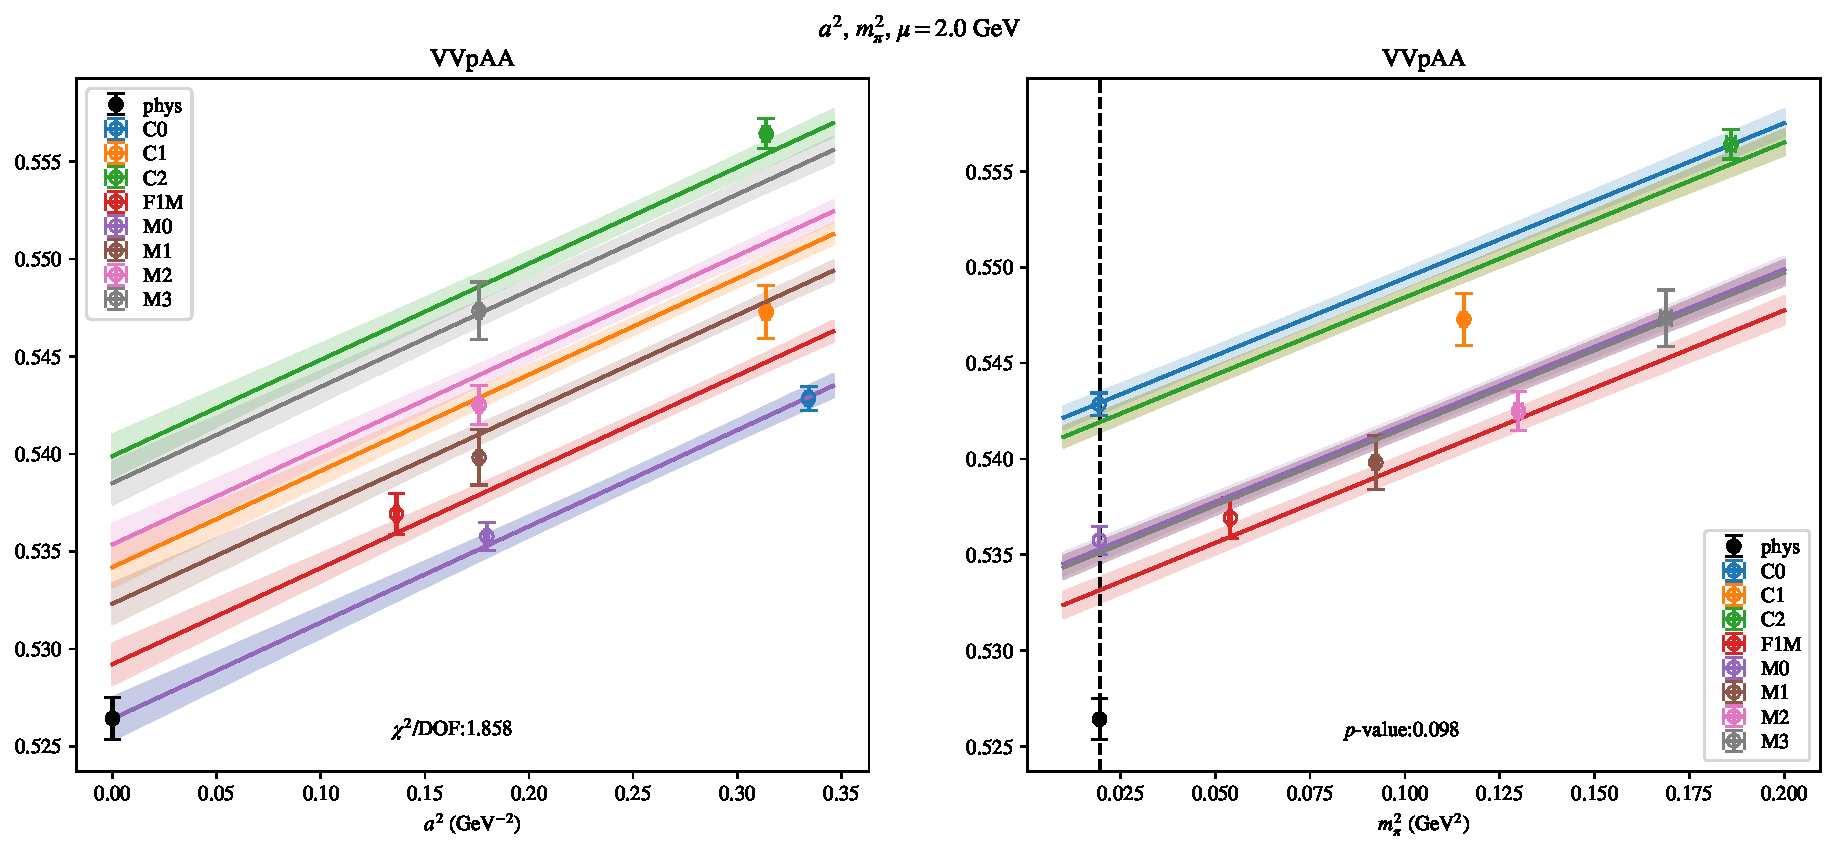
\includepdf[link, pages=-]{VVpAA/SUSY_F/a2m2_20.pdf}
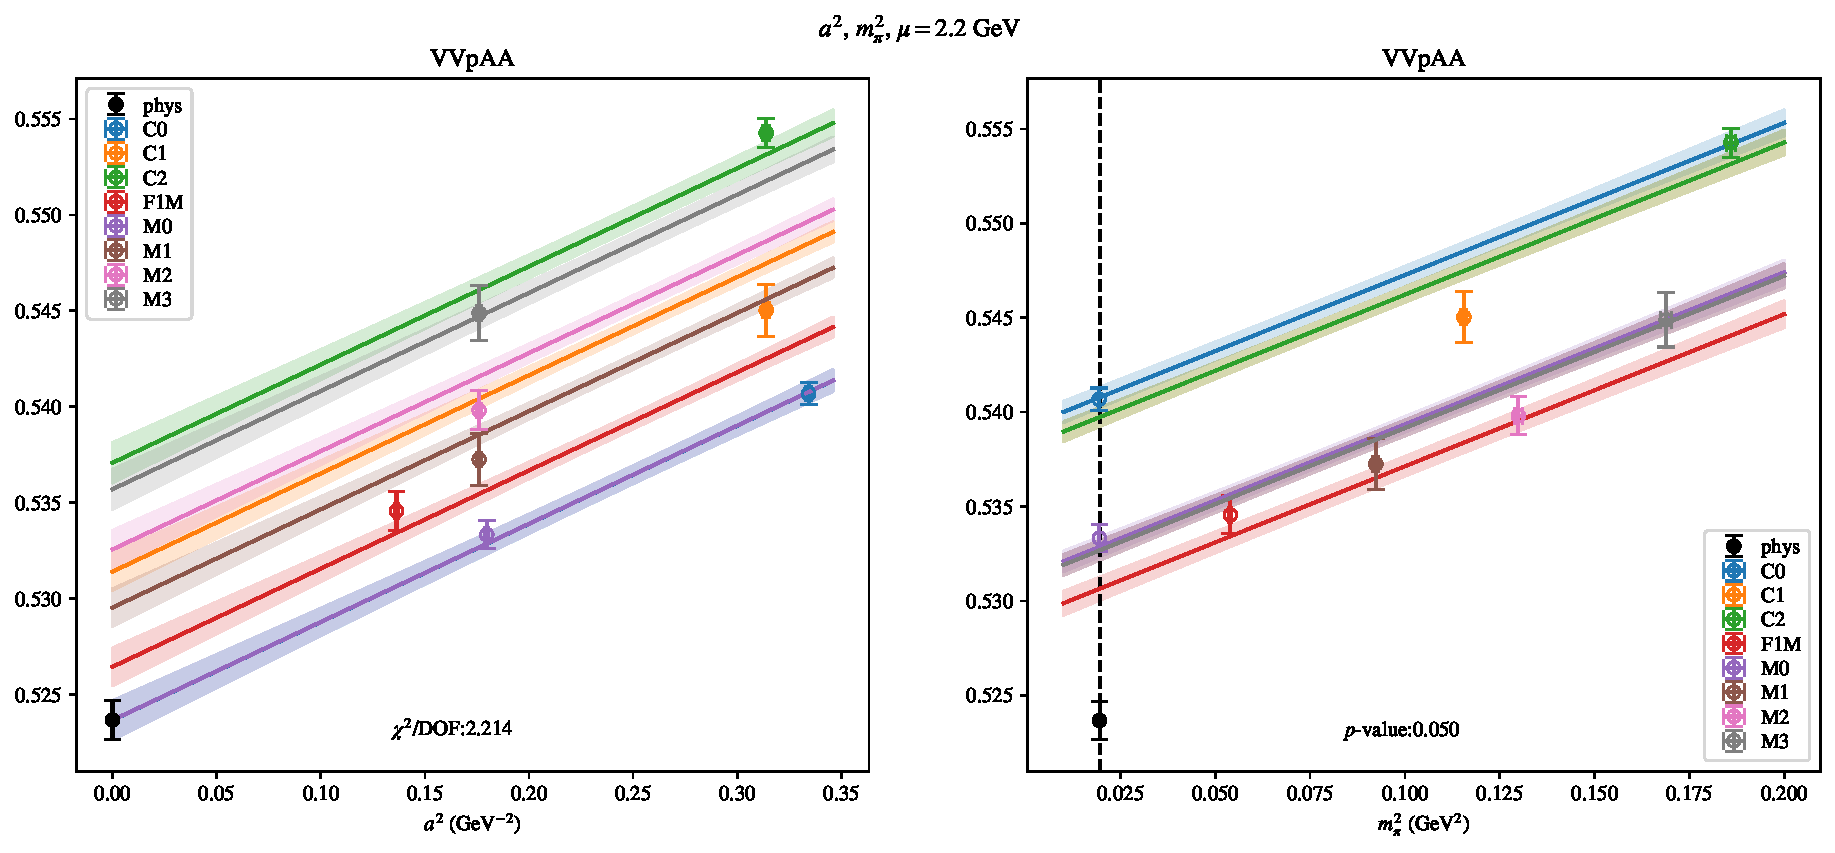
\includepdf[link, pages=-]{VVpAA/SUSY_F/a2m2_22.pdf}
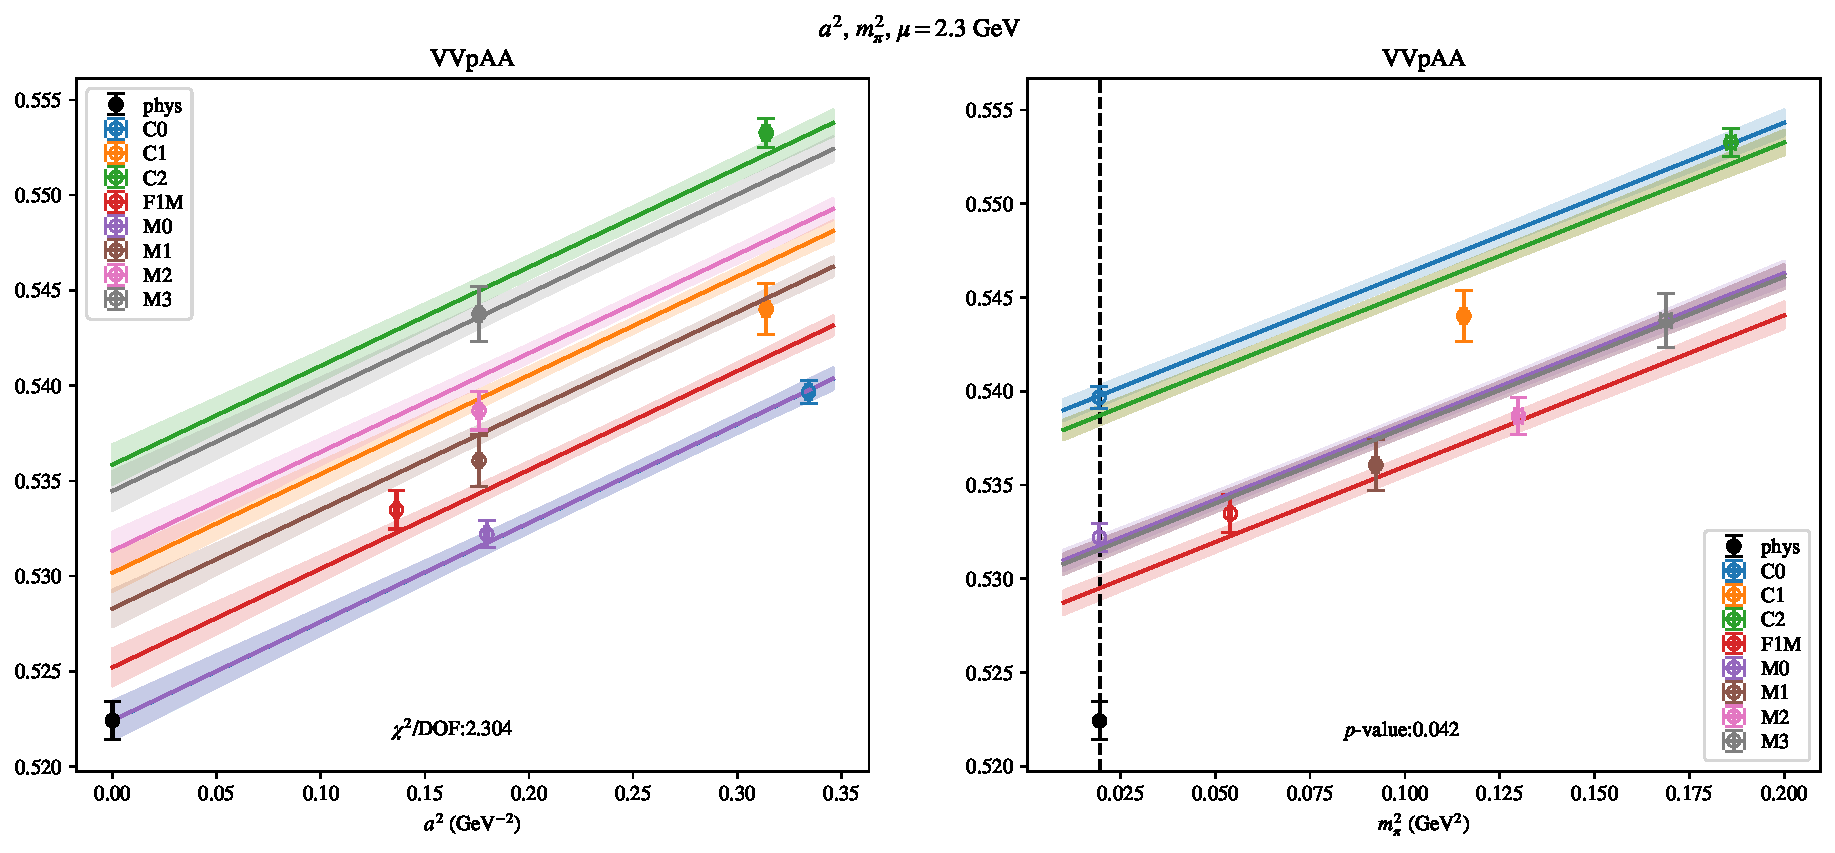
\includepdf[link, pages=-]{VVpAA/SUSY_F/a2m2_23.pdf}
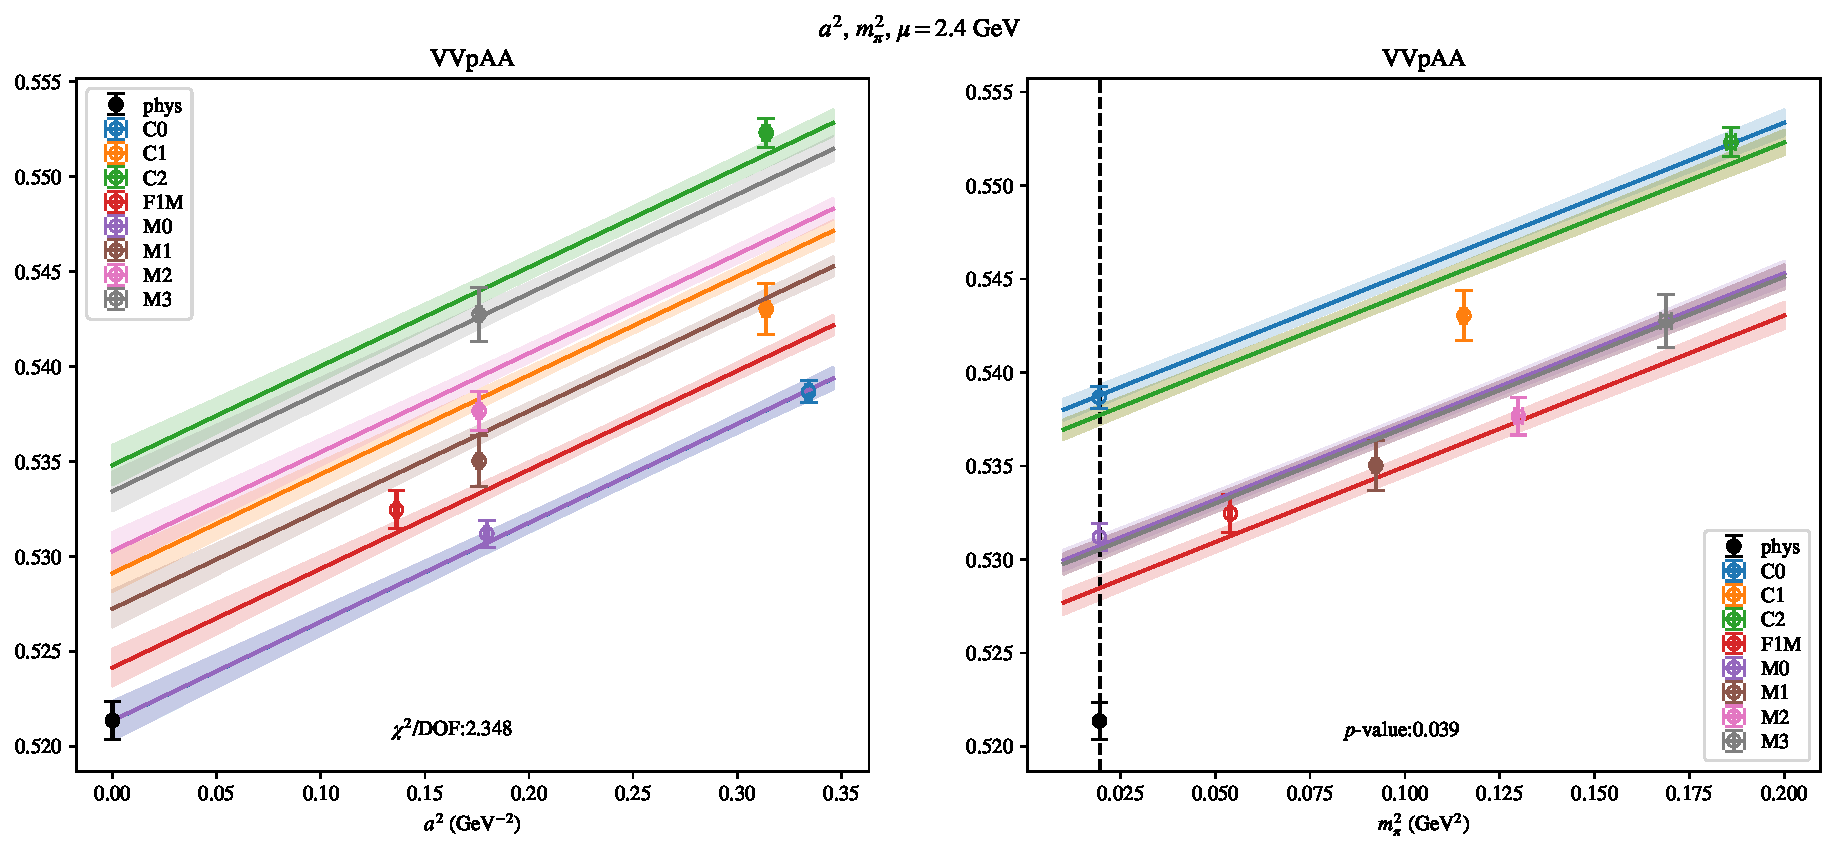
\includepdf[link, pages=-]{VVpAA/SUSY_F/a2m2_24.pdf}
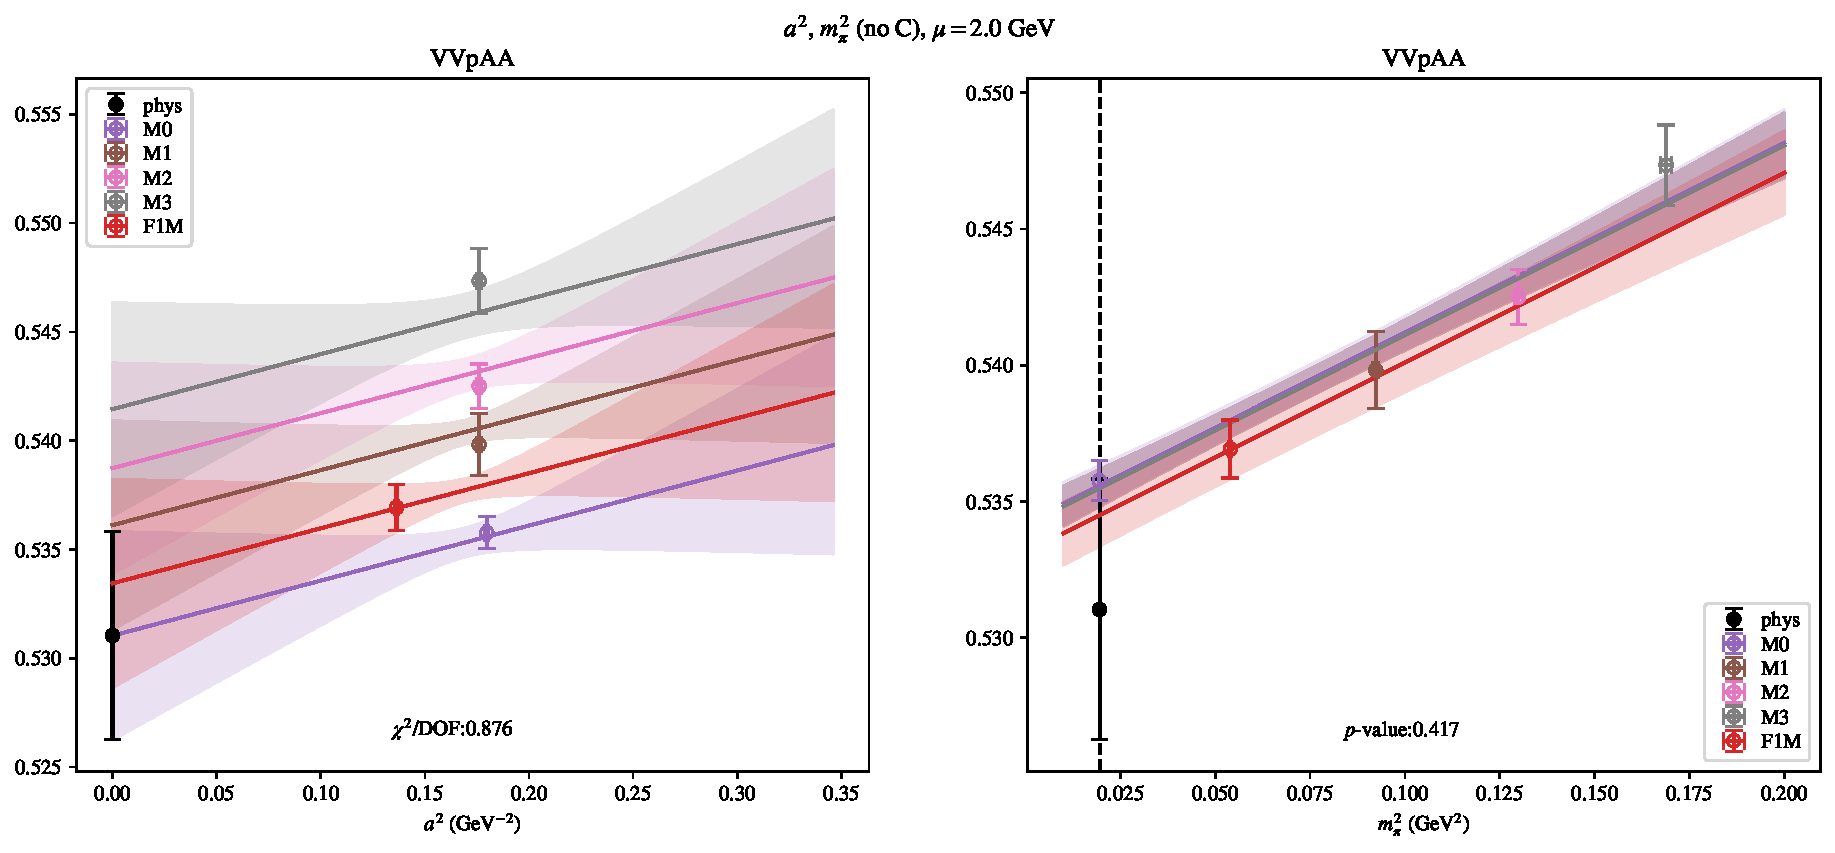
\includepdf[link, pages=-]{VVpAA/SUSY_F/a2m2noC_20.pdf}
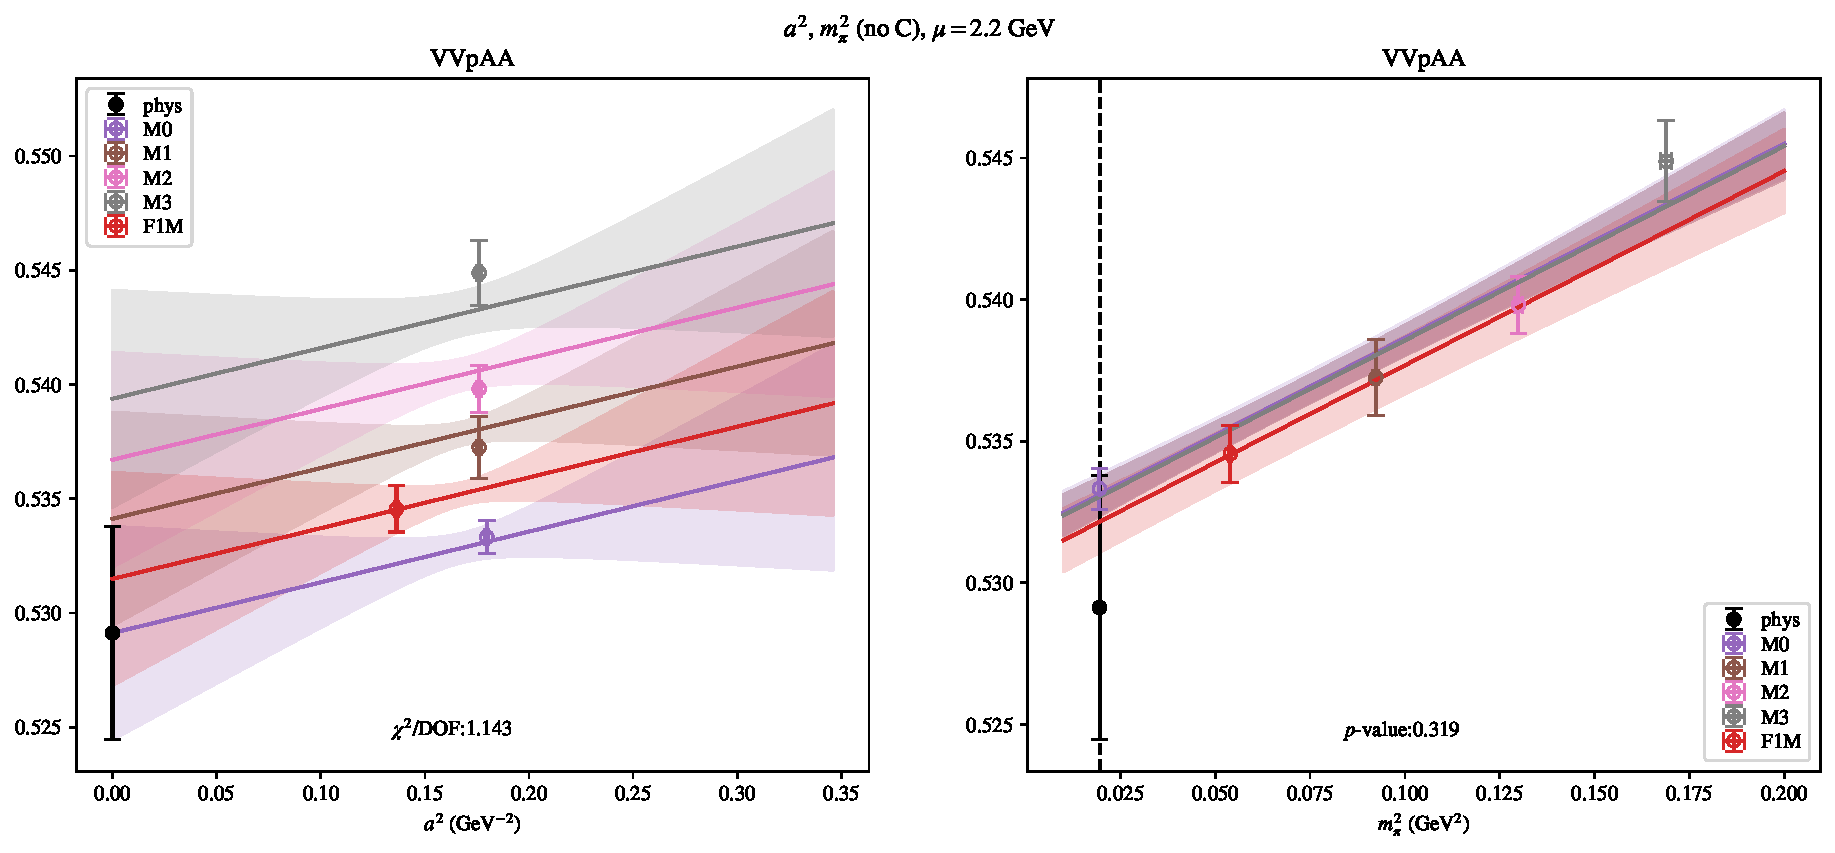
\includepdf[link, pages=-]{VVpAA/SUSY_F/a2m2noC_22.pdf}
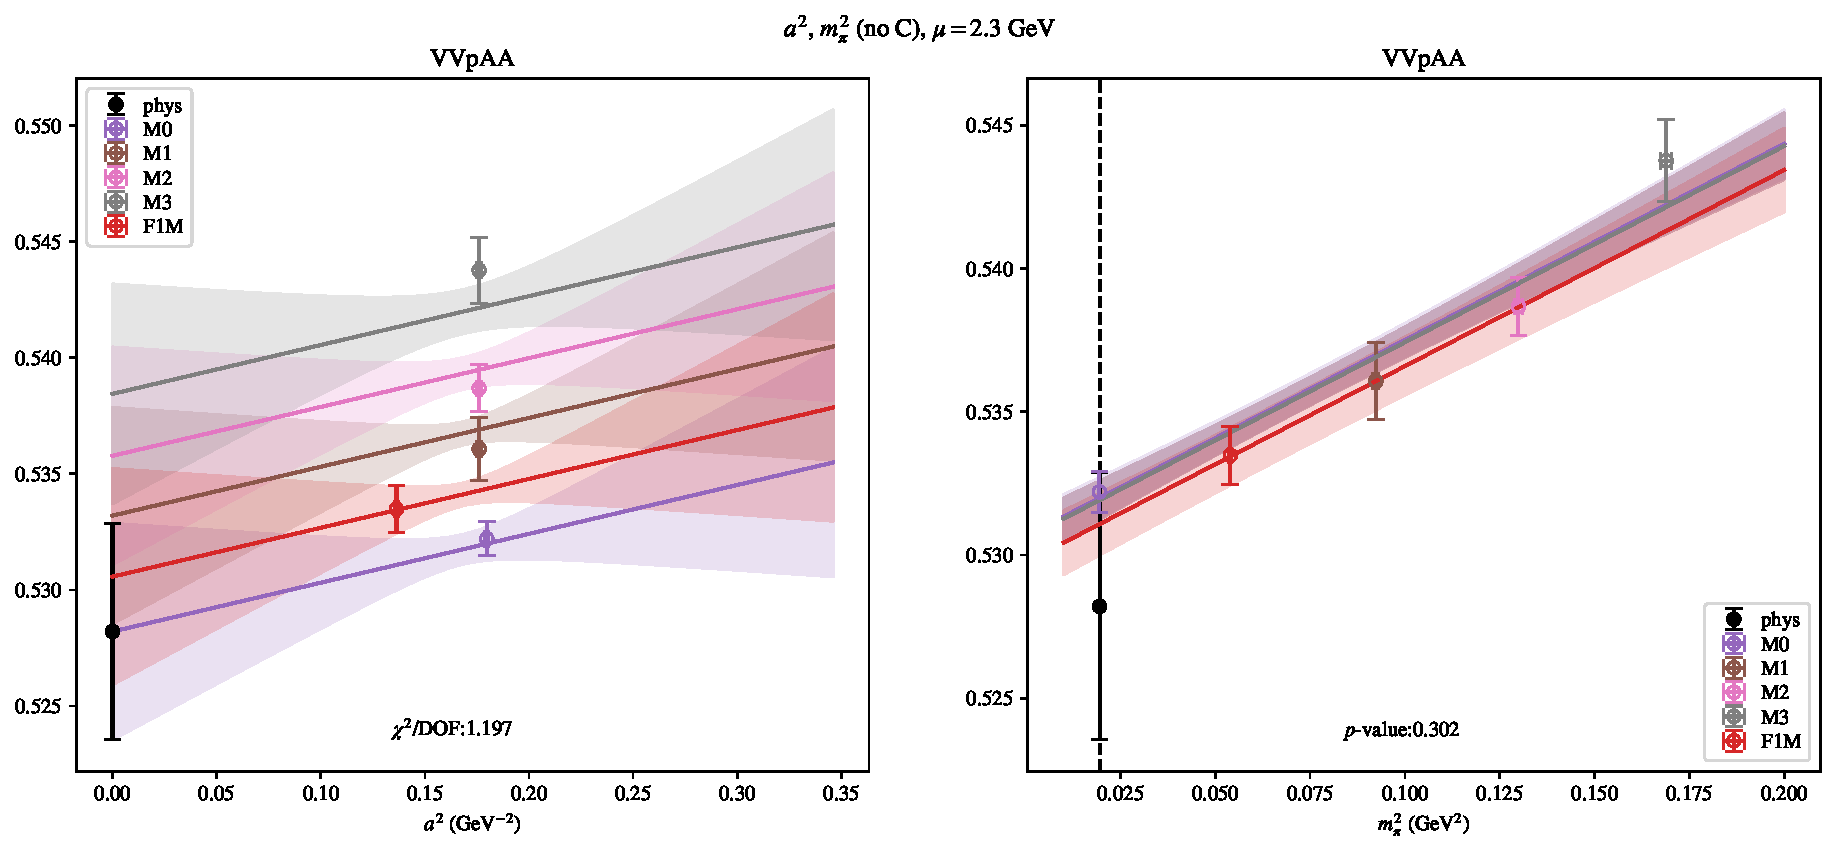
\includepdf[link, pages=-]{VVpAA/SUSY_F/a2m2noC_23.pdf}
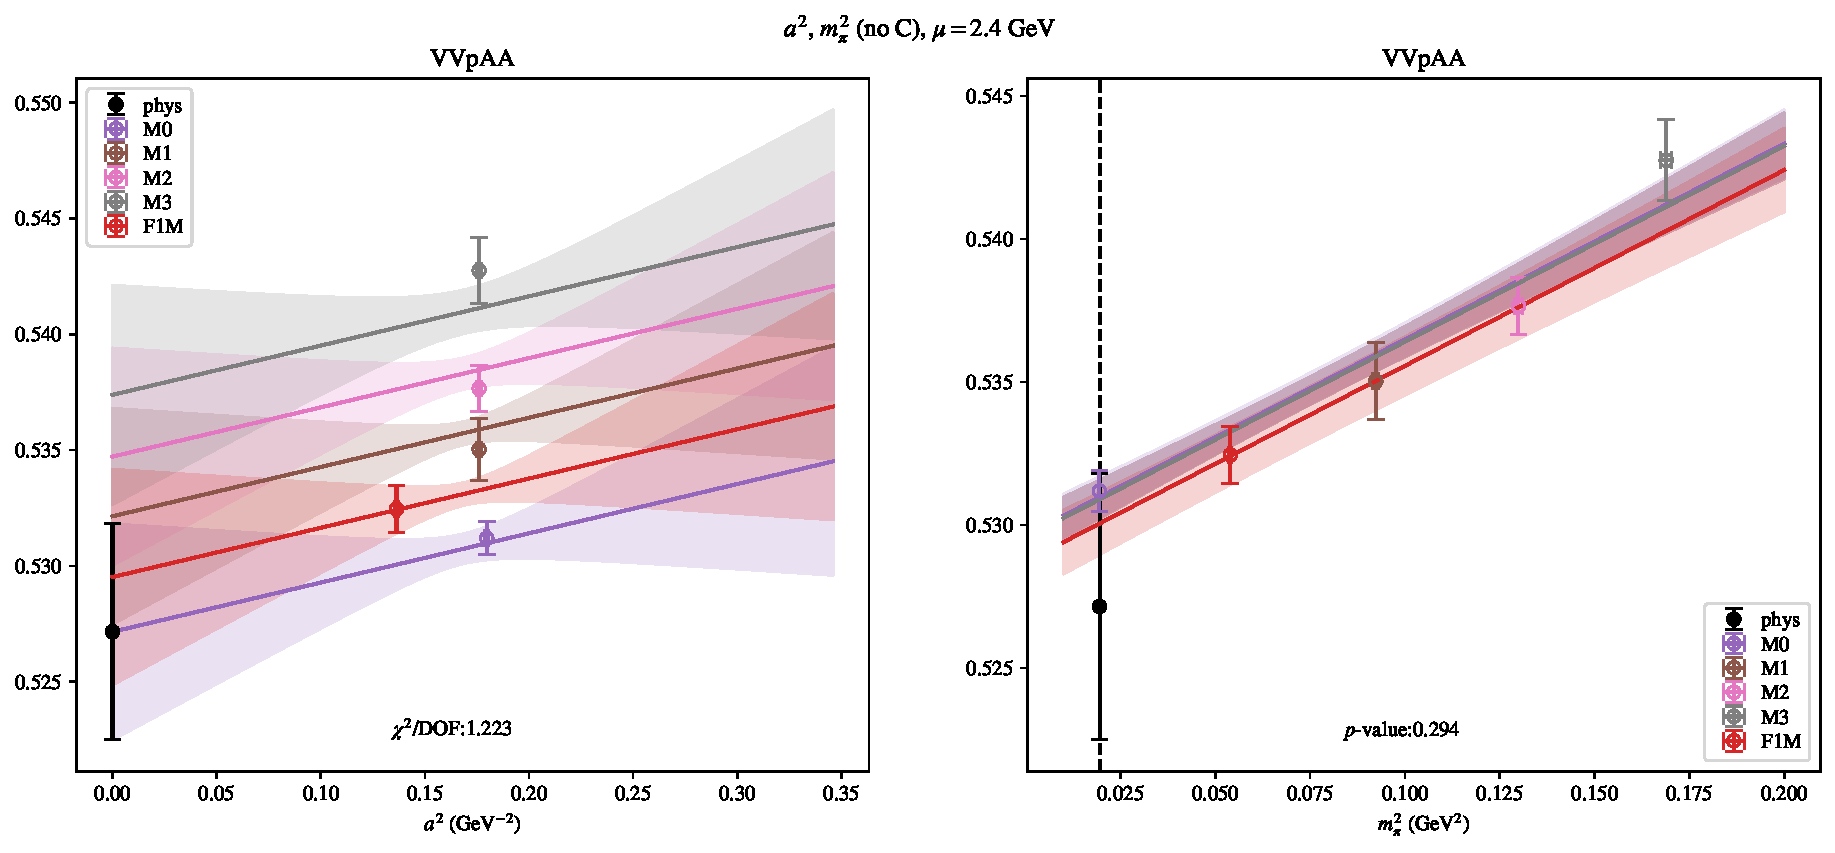
\includepdf[link, pages=-]{VVpAA/SUSY_F/a2m2noC_24.pdf}
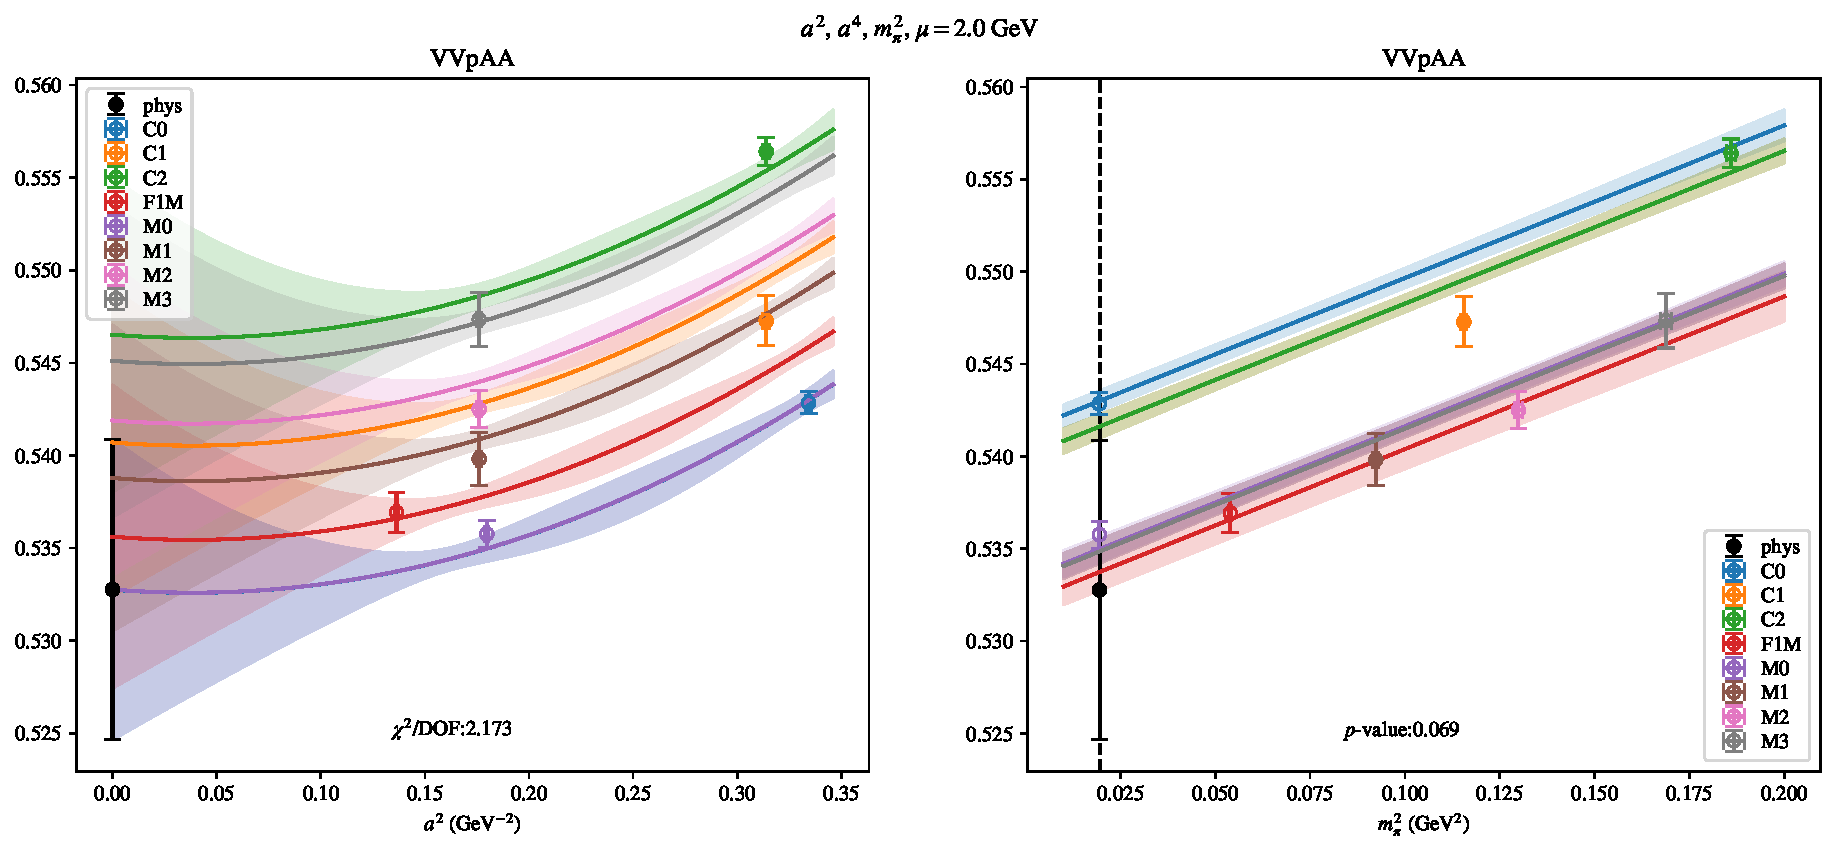
\includepdf[link, pages=-]{VVpAA/SUSY_F/a2a4m2_20.pdf}
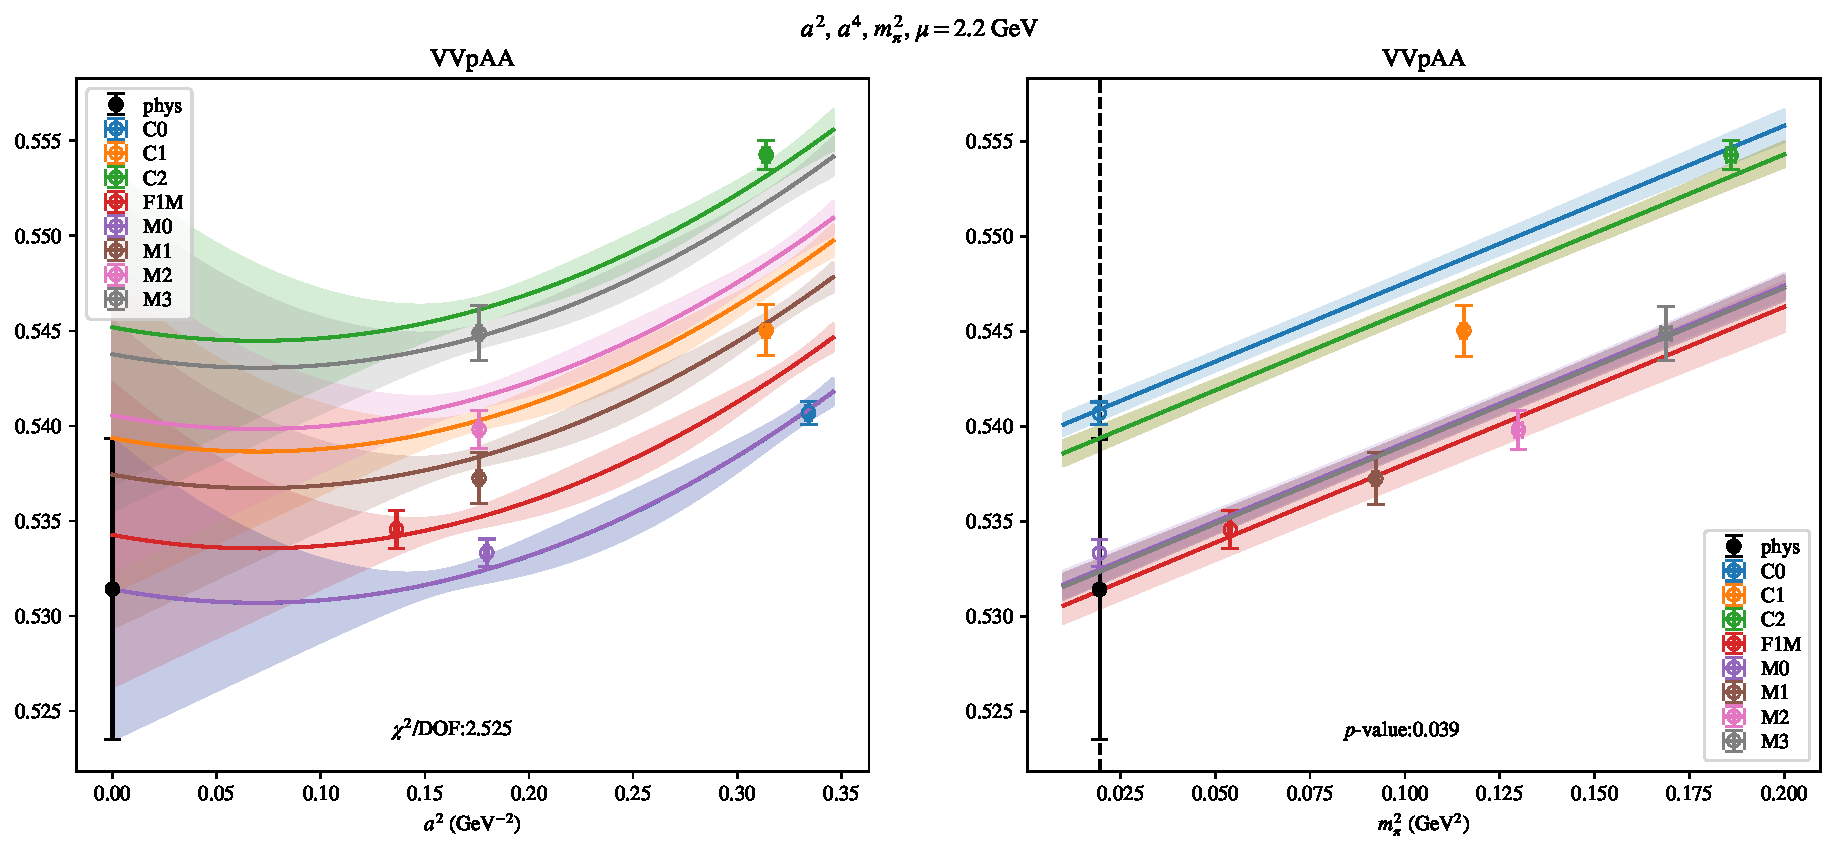
\includepdf[link, pages=-]{VVpAA/SUSY_F/a2a4m2_22.pdf}
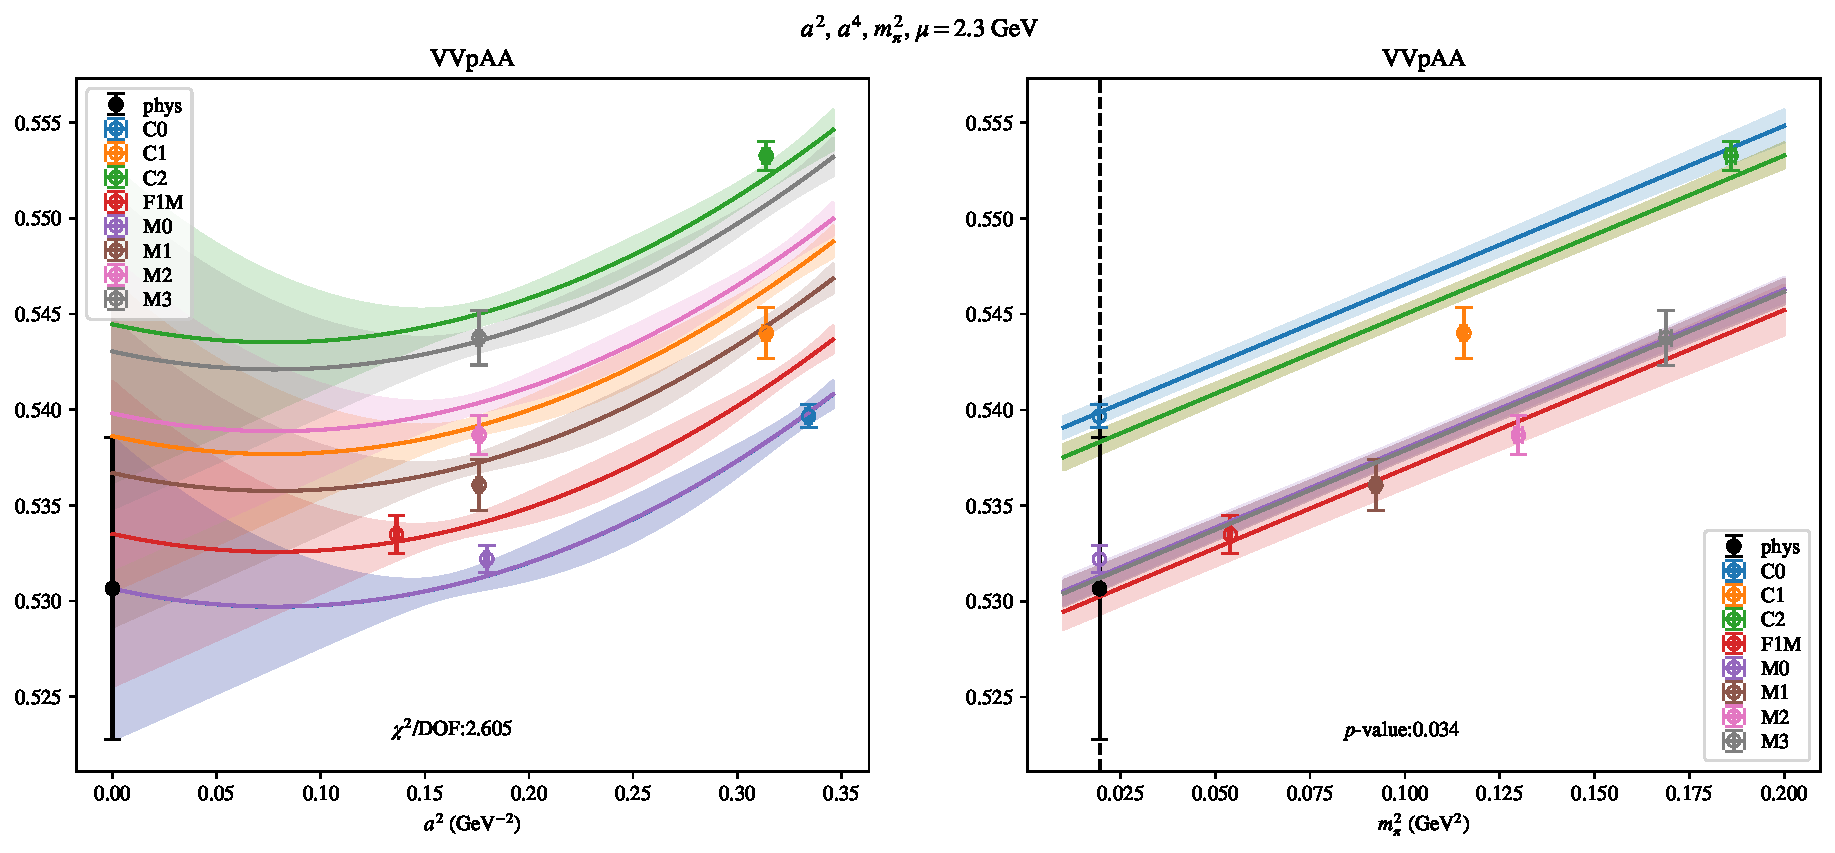
\includepdf[link, pages=-]{VVpAA/SUSY_F/a2a4m2_23.pdf}
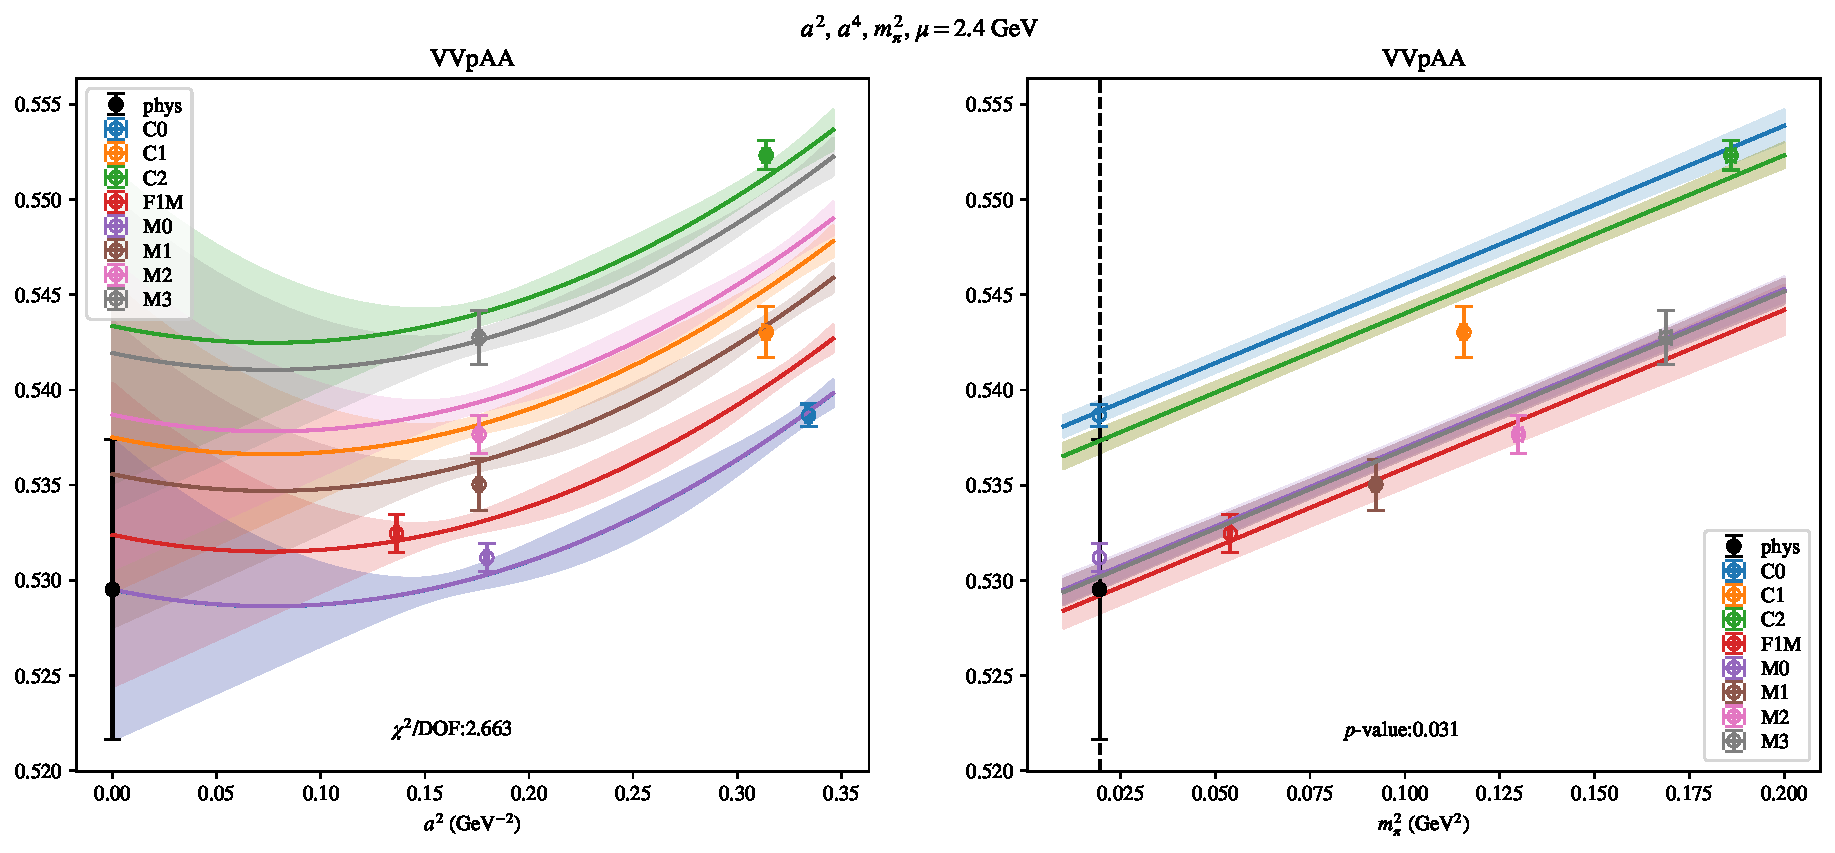
\includepdf[link, pages=-]{VVpAA/SUSY_F/a2a4m2_24.pdf}
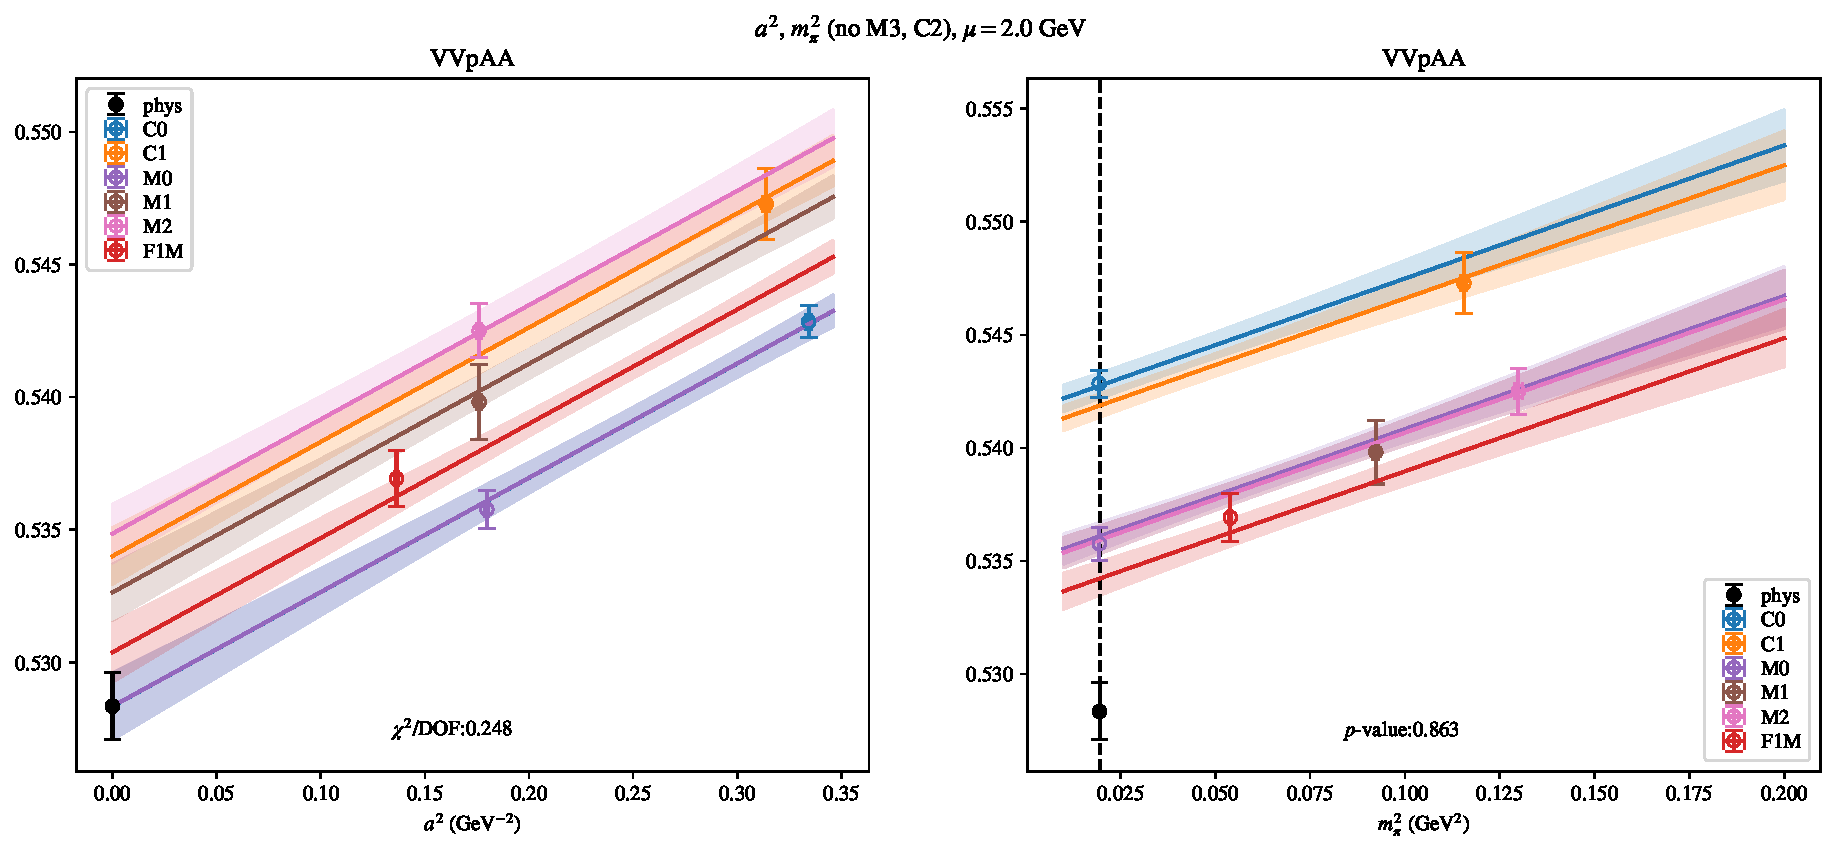
\includepdf[link, pages=-]{VVpAA/SUSY_F/a2m2mcut_20.pdf}
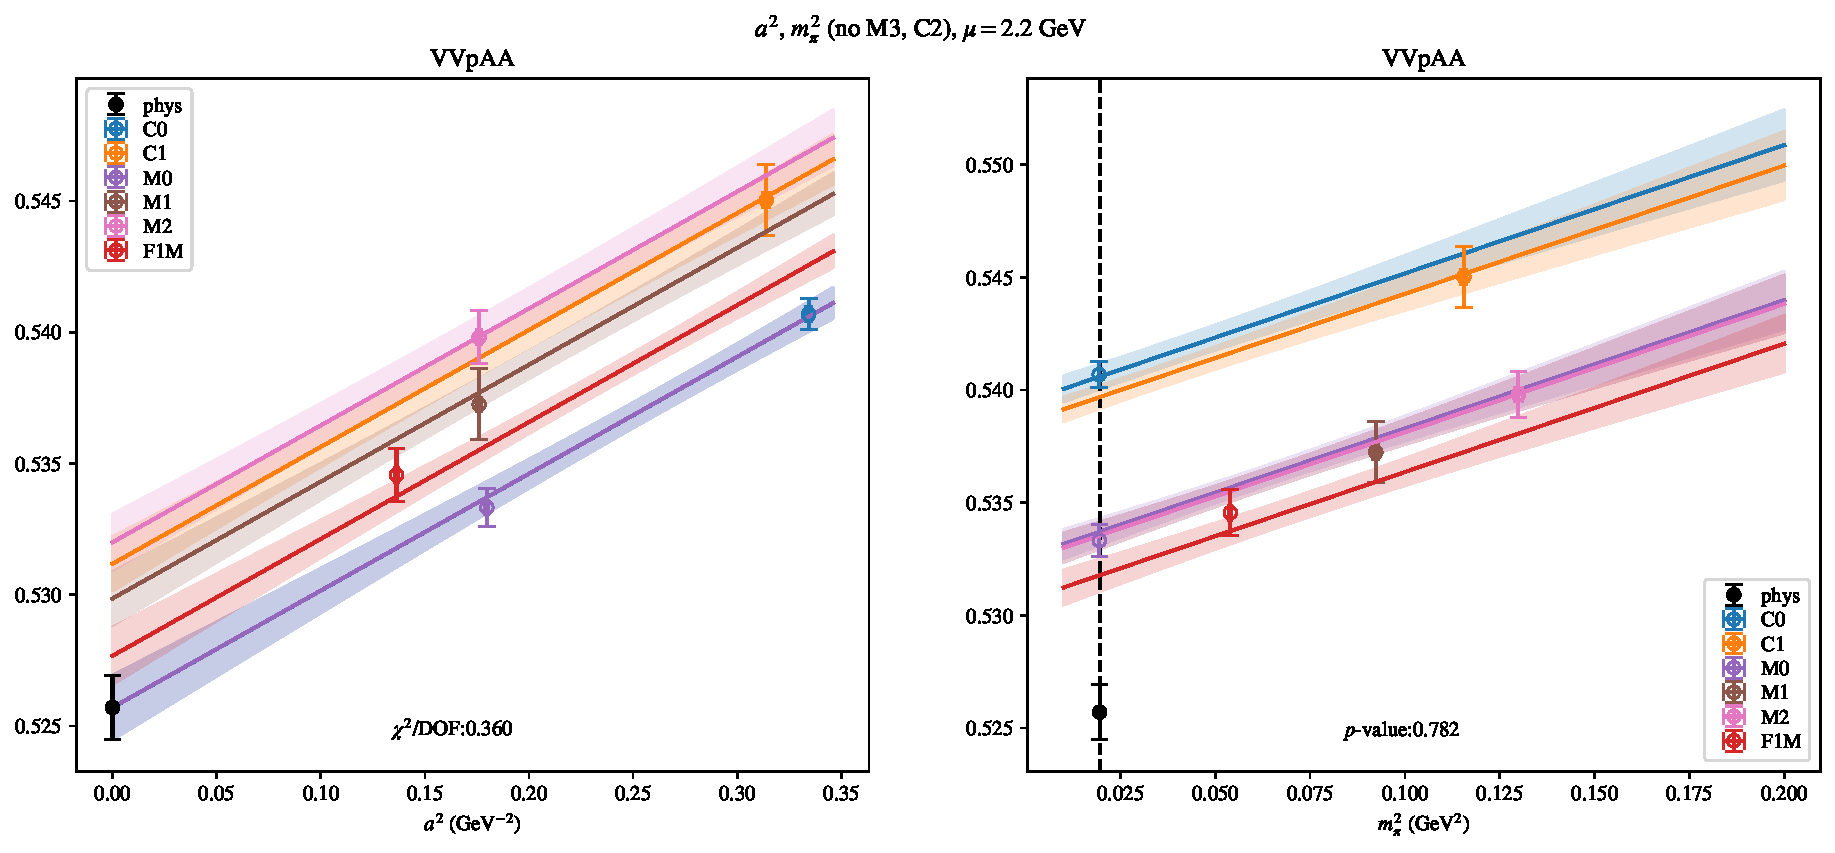
\includepdf[link, pages=-]{VVpAA/SUSY_F/a2m2mcut_22.pdf}
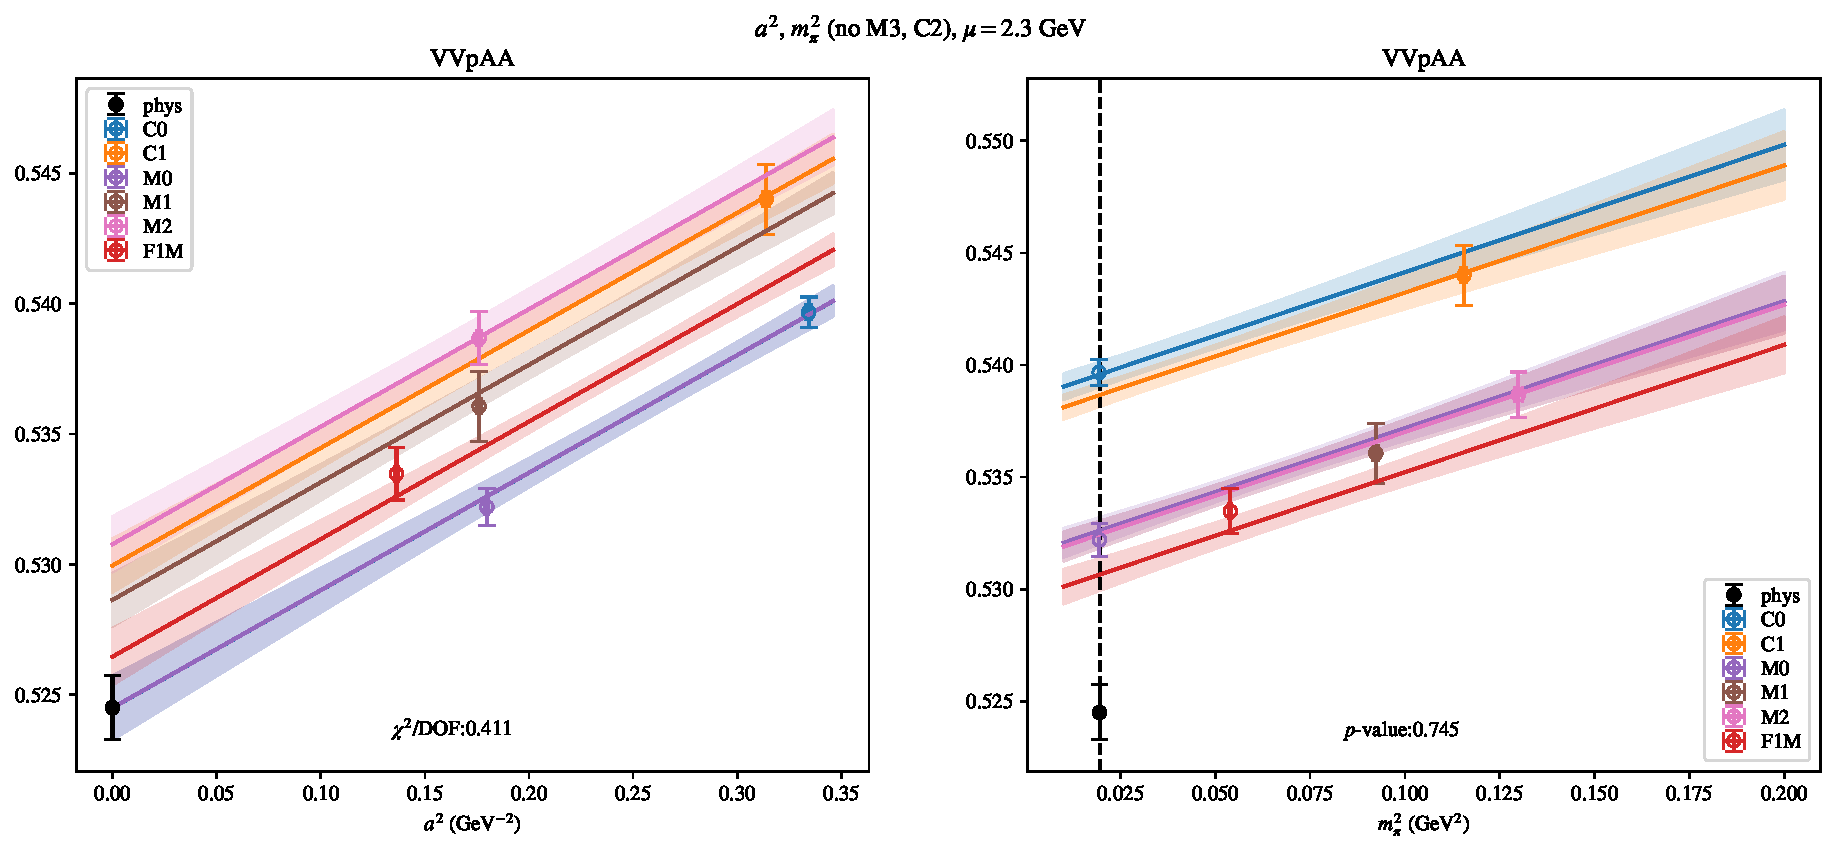
\includepdf[link, pages=-]{VVpAA/SUSY_F/a2m2mcut_23.pdf}
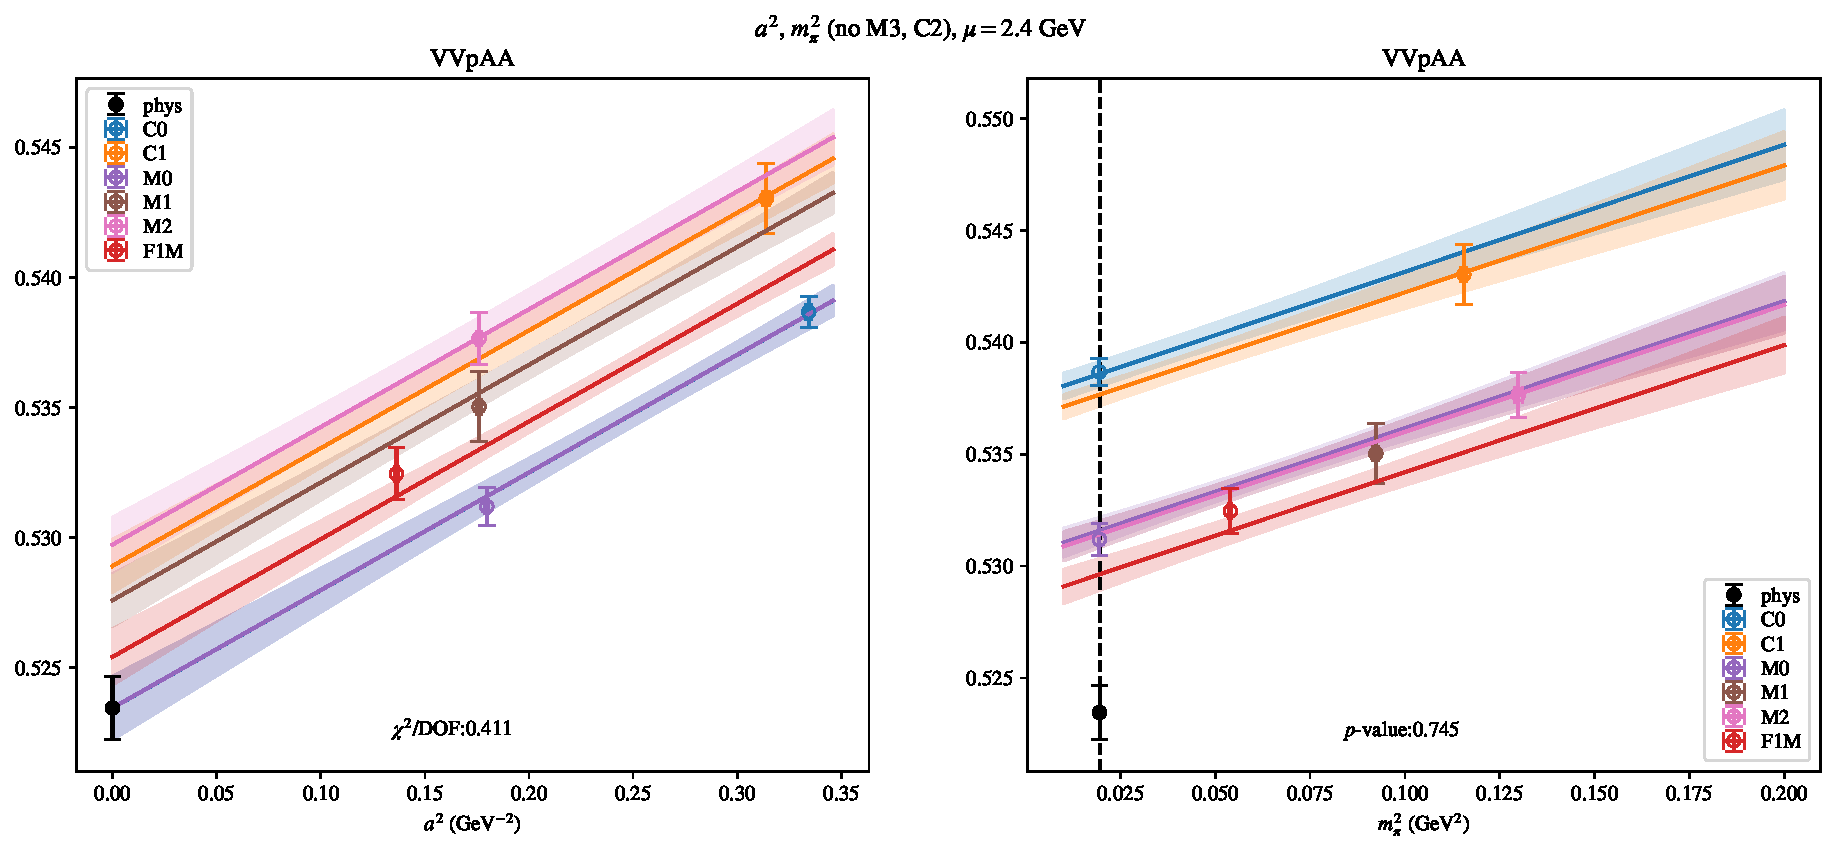
\includepdf[link, pages=-]{VVpAA/SUSY_F/a2m2mcut_24.pdf}
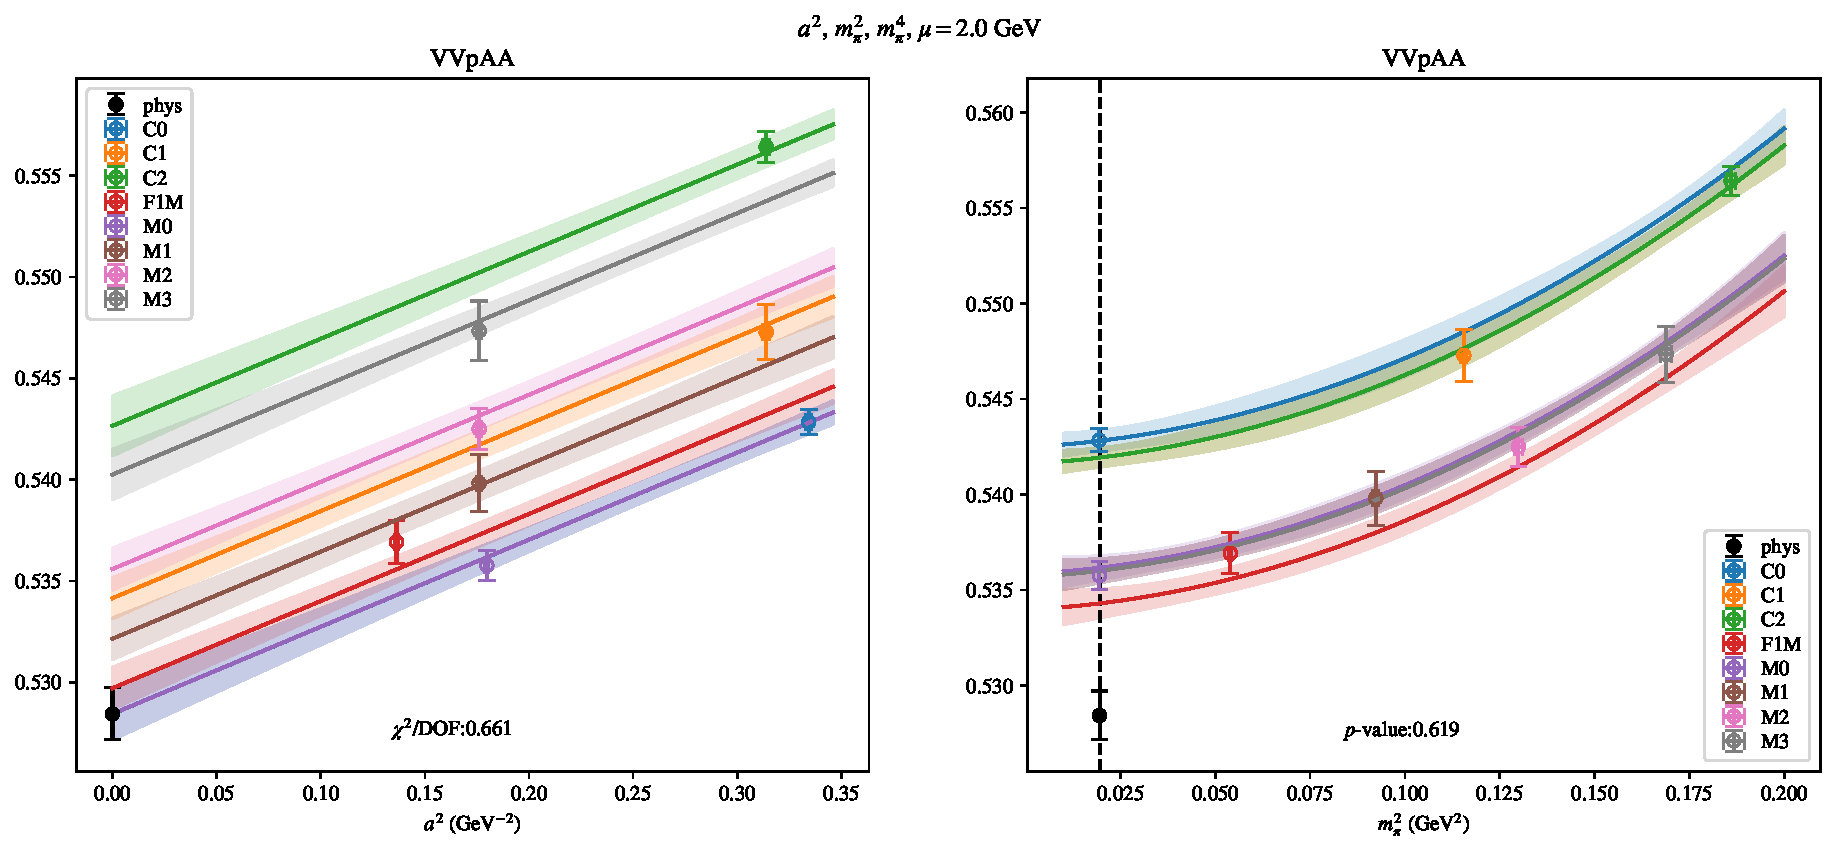
\includepdf[link, pages=-]{VVpAA/SUSY_F/a2m2m4_20.pdf}
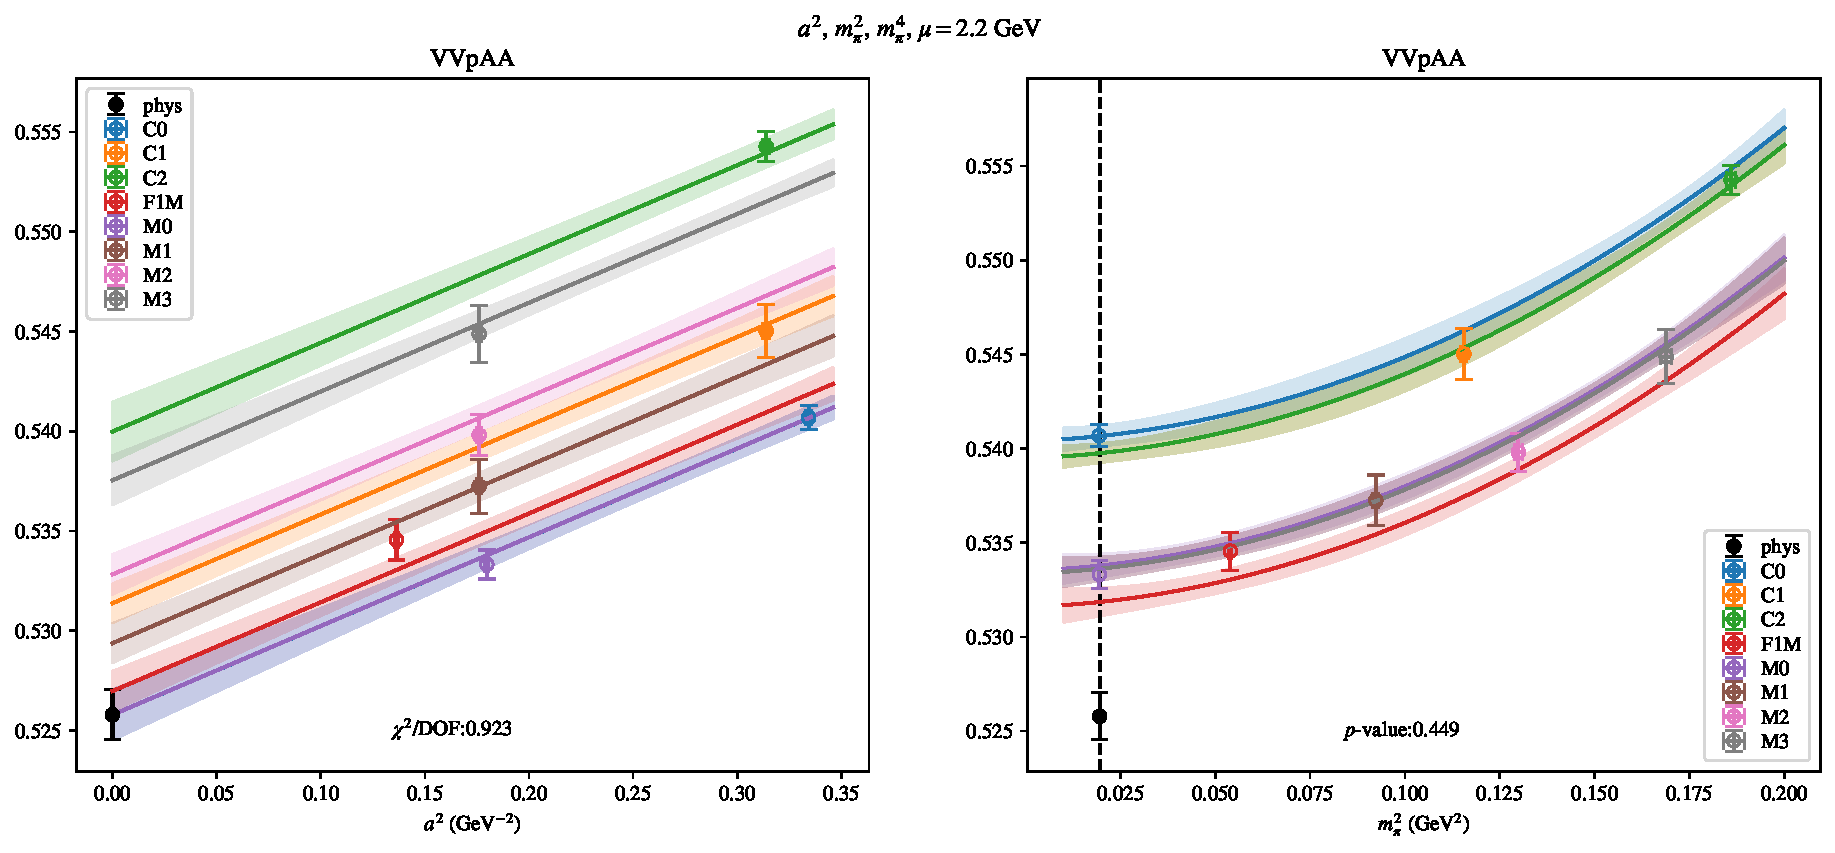
\includepdf[link, pages=-]{VVpAA/SUSY_F/a2m2m4_22.pdf}
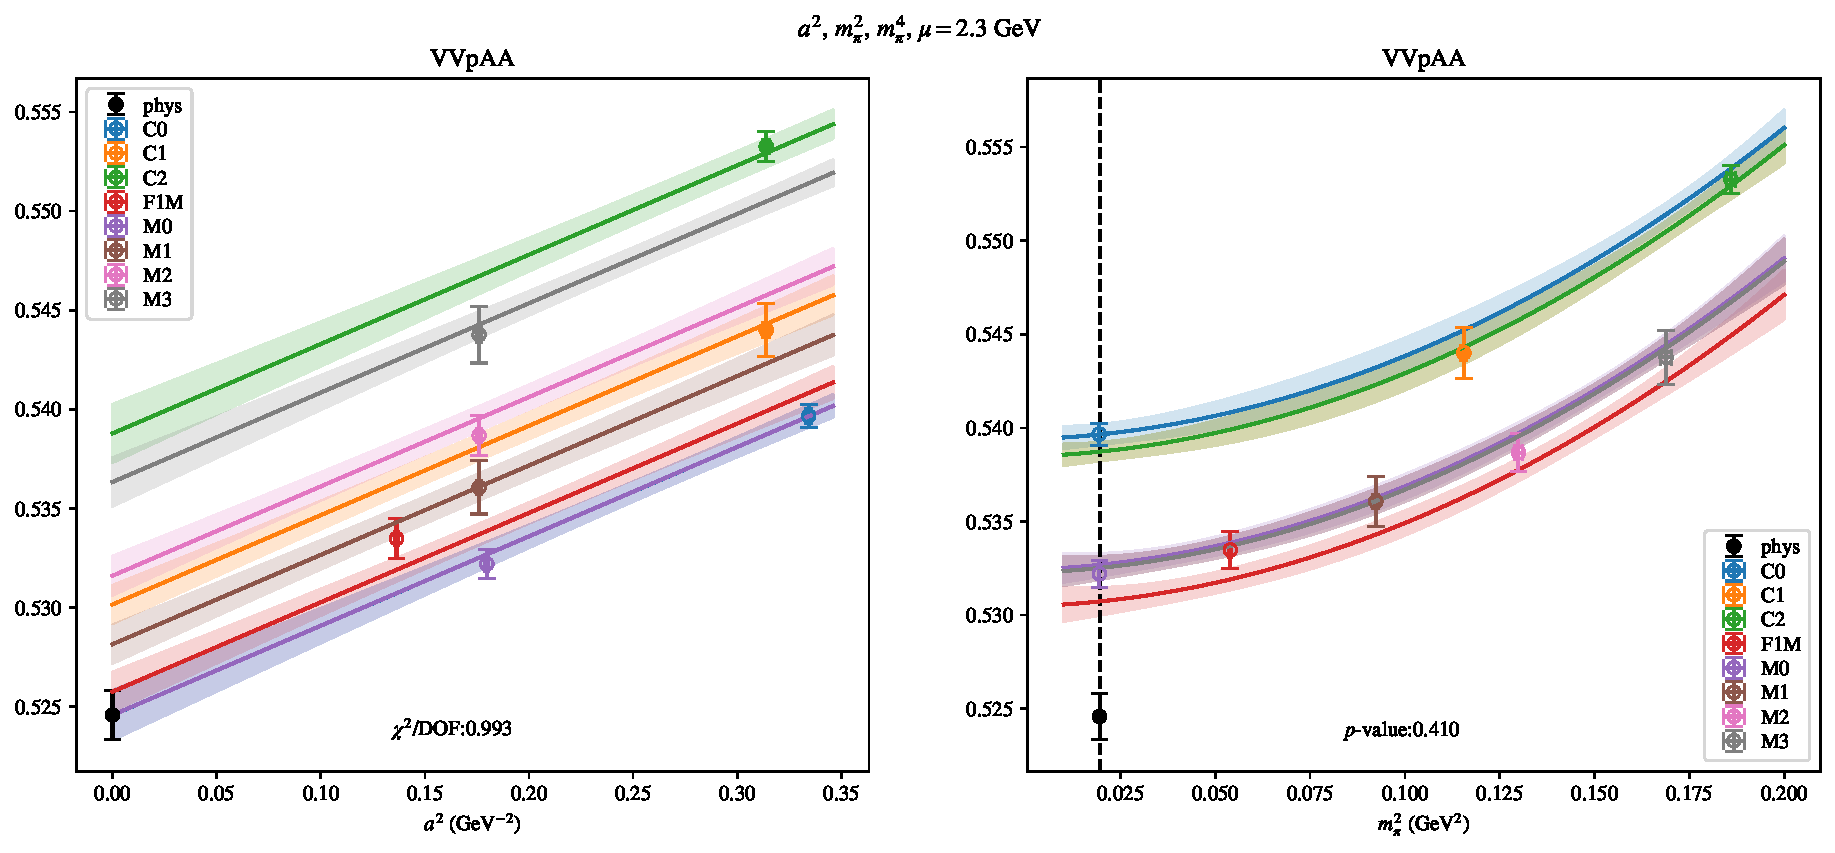
\includepdf[link, pages=-]{VVpAA/SUSY_F/a2m2m4_23.pdf}
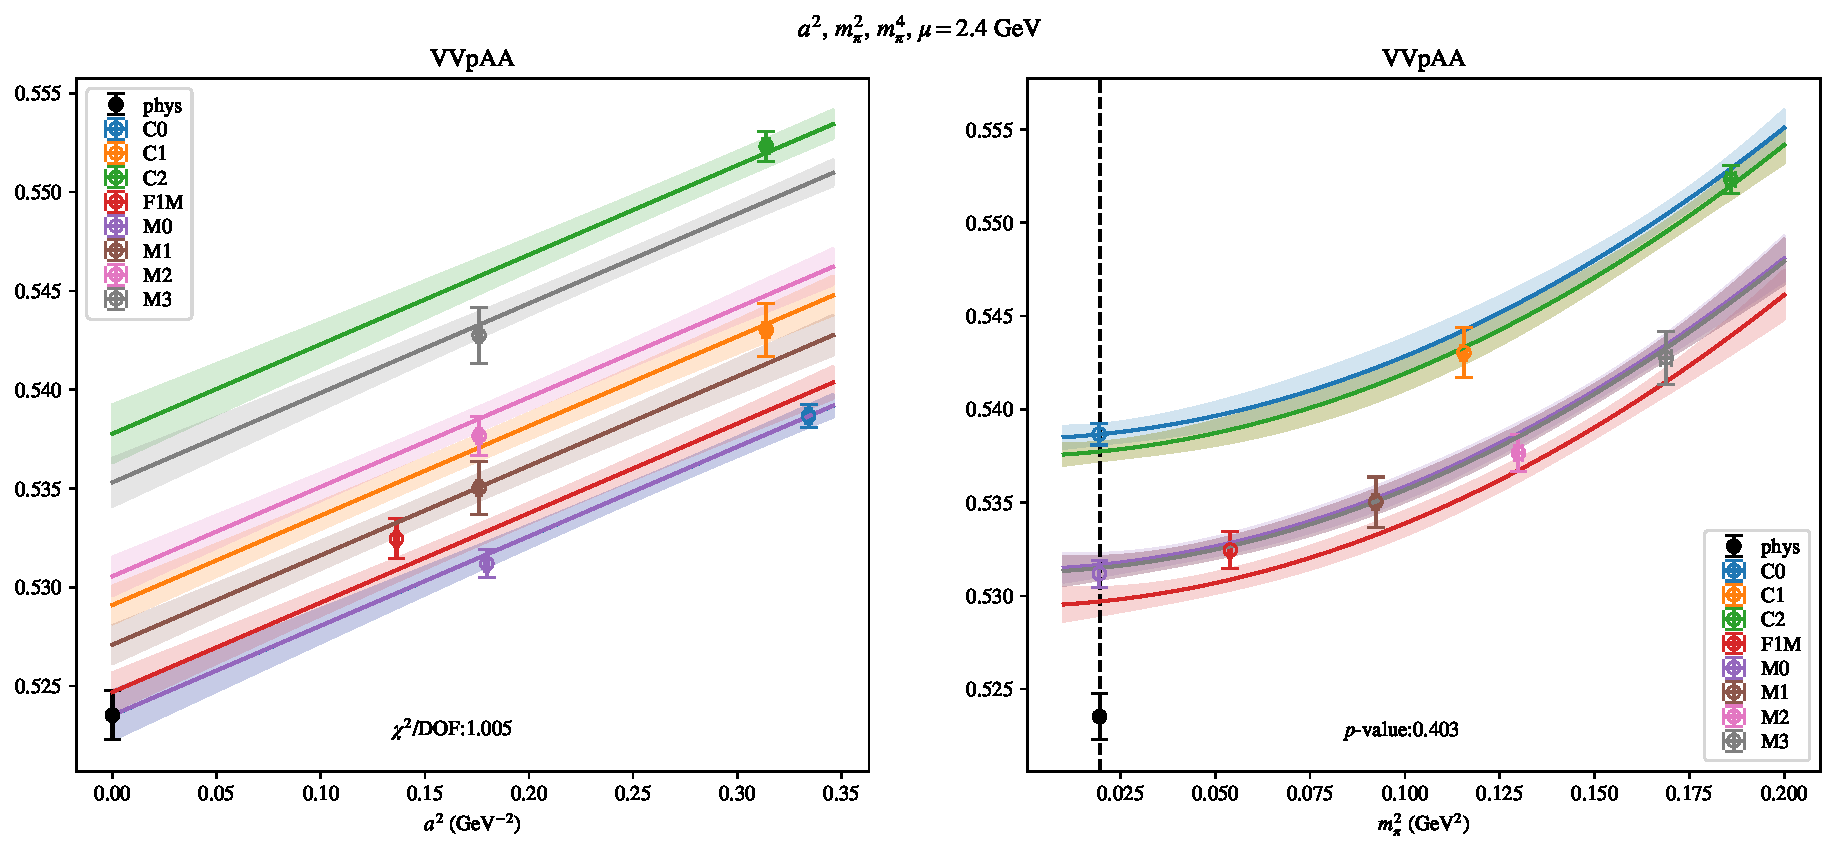
\includepdf[link, pages=-]{VVpAA/SUSY_F/a2m2m4_24.pdf}
\clearpage
\section{$B_2$}
\begin{table}[h!]
\begin{center}
\begin{tabular}{|c|c|c|c|c|c|}
\hline
$\mu$ (GeV) & $a^2$, $m_\pi^2$& $a^2$, $m_\pi^2$ (no C)& $a^2$, $a^4$, $m_\pi^2$& $a^2$, $m_\pi^2$ (no M3, C2)& $a^2$, $m_\pi^2$, $m_\pi^4$\\
\hline
2.0& \hyperlink{VVmAA/SUSY_F/a2m2_20.pdf.1}{\textbf{-0.970(44)}: 7.006 (0.0)} & \hyperlink{VVmAA/SUSY_F/a2m2noC_20.pdf.1}{\textbf{-1.054(97)}: 1.477 (0.228)} & \hyperlink{VVmAA/SUSY_F/a2a4m2_20.pdf.1}{\textbf{-1.11(15)}: 1.501 (0.199)} & \hyperlink{VVmAA/SUSY_F/a2m2mcut_20.pdf.1}{\textbf{-0.968(42)}: 11.144 (0.0)} & \hyperlink{VVmAA/SUSY_F/a2m2m4_20.pdf.1}{\textbf{-0.965(42)}: 7.095 (0.0)}\\
2.2& \hyperlink{VVmAA/SUSY_F/a2m2_22.pdf.1}{\textbf{-0.850(43)}: 6.344 (0.0)} & \hyperlink{VVmAA/SUSY_F/a2m2noC_22.pdf.1}{\textbf{-0.935(98)}: 0.972 (0.378)} & \hyperlink{VVmAA/SUSY_F/a2a4m2_22.pdf.1}{\textbf{-0.98(15)}: 1.8 (0.126)} & \hyperlink{VVmAA/SUSY_F/a2m2mcut_22.pdf.1}{\textbf{-0.849(42)}: 9.893 (0.0)} & \hyperlink{VVmAA/SUSY_F/a2m2m4_22.pdf.1}{\textbf{-0.846(41)}: 6.425 (0.0)}\\
2.3& \hyperlink{VVmAA/SUSY_F/a2m2_23.pdf.1}{\textbf{-0.801(38)}: 7.974 (0.0)} & \hyperlink{VVmAA/SUSY_F/a2m2noC_23.pdf.1}{\textbf{-0.887(89)}: 0.803 (0.448)} & \hyperlink{VVmAA/SUSY_F/a2a4m2_23.pdf.1}{\textbf{-0.94(13)}: 1.587 (0.175)} & \hyperlink{VVmAA/SUSY_F/a2m2mcut_23.pdf.1}{\textbf{-0.800(37)}: 12.521 (0.0)} & \hyperlink{VVmAA/SUSY_F/a2m2m4_23.pdf.1}{\textbf{-0.797(36)}: 8.053 (0.0)}\\
2.4& \hyperlink{VVmAA/SUSY_F/a2m2_24.pdf.1}{\textbf{-0.762(36)}: 6.868 (0.0)} & \hyperlink{VVmAA/SUSY_F/a2m2noC_24.pdf.1}{\textbf{-0.835(82)}: 0.706 (0.494)} & \hyperlink{VVmAA/SUSY_F/a2a4m2_24.pdf.1}{\textbf{-0.87(12)}: 1.999 (0.092)} & \hyperlink{VVmAA/SUSY_F/a2m2mcut_24.pdf.1}{\textbf{-0.762(36)}: 10.826 (0.0)} & \hyperlink{VVmAA/SUSY_F/a2m2m4_24.pdf.1}{\textbf{-0.759(35)}: 7.078 (0.0)}\\
\hline
\end{tabular}
\caption{Physical point value from chiral and continuum extrapolation at renormalisation scale $\mu$. Entries are \textbf{value(error)}: $\chi^2/\text{DOF}$ ($p$-value).}
\end{center}
\end{table}
\begin{table}[h!]
\begin{center}
\begin{tabular}{|c c|c|c|c|c|c|}
\hline
$\mu$ (GeV) &  & $a^2$, $m_\pi^2$& $a^2$, $m_\pi^2$ (no C)& $a^2$, $a^4$, $m_\pi^2$& $a^2$, $m_\pi^2$ (no M3, C2)& $a^2$, $m_\pi^2$, $m_\pi^4$\\
\hline
\multirow{2}{0.5in}{2.0} & $\alpha$ & -0.781(45)& -1.20(41)& -1.89(98)& -0.777(50)& -0.771(47)\\
 & $\beta$ & 0.00631(17)& 0.00657(25)& 0.00619(15)& 0.00681(26)& 0.00989(61)\\
\hline
\multirow{2}{0.5in}{2.2} & $\alpha$ & -0.760(50)& -1.23(40)& -1.89(95)& -0.759(53)& -0.751(50)\\
 & $\beta$ & 0.00616(14)& 0.00601(21)& 0.00601(12)& 0.00670(25)& 0.00946(64)\\
\hline
\multirow{2}{0.5in}{2.3} & $\alpha$ & -0.747(51)& -1.25(39)& -1.98(92)& -0.744(52)& -0.737(49)\\
 & $\beta$ & 0.00608(19)& 0.00600(26)& 0.00591(15)& 0.00667(31)& 0.00990(72)\\
\hline
\multirow{2}{0.5in}{2.4} & $\alpha$ & -0.749(51)& -1.20(40)& -1.84(97)& -0.748(55)& -0.740(51)\\
 & $\beta$ & 0.00609(14)& 0.00595(20)& 0.00600(12)& 0.00656(24)& 0.00925(62)\\
\hline
\end{tabular}
\caption{Fit values of coefficients in $B = B_{phys} + \mathbf{\alpha} a^2 + \mathbf{\beta}\left(\frac{m_\pi^2}{f_\pi^2}-\frac{m_{\pi,PDG}^2}{f_\pi^2}\right) + \ldots$.}
\end{center}
\end{table}
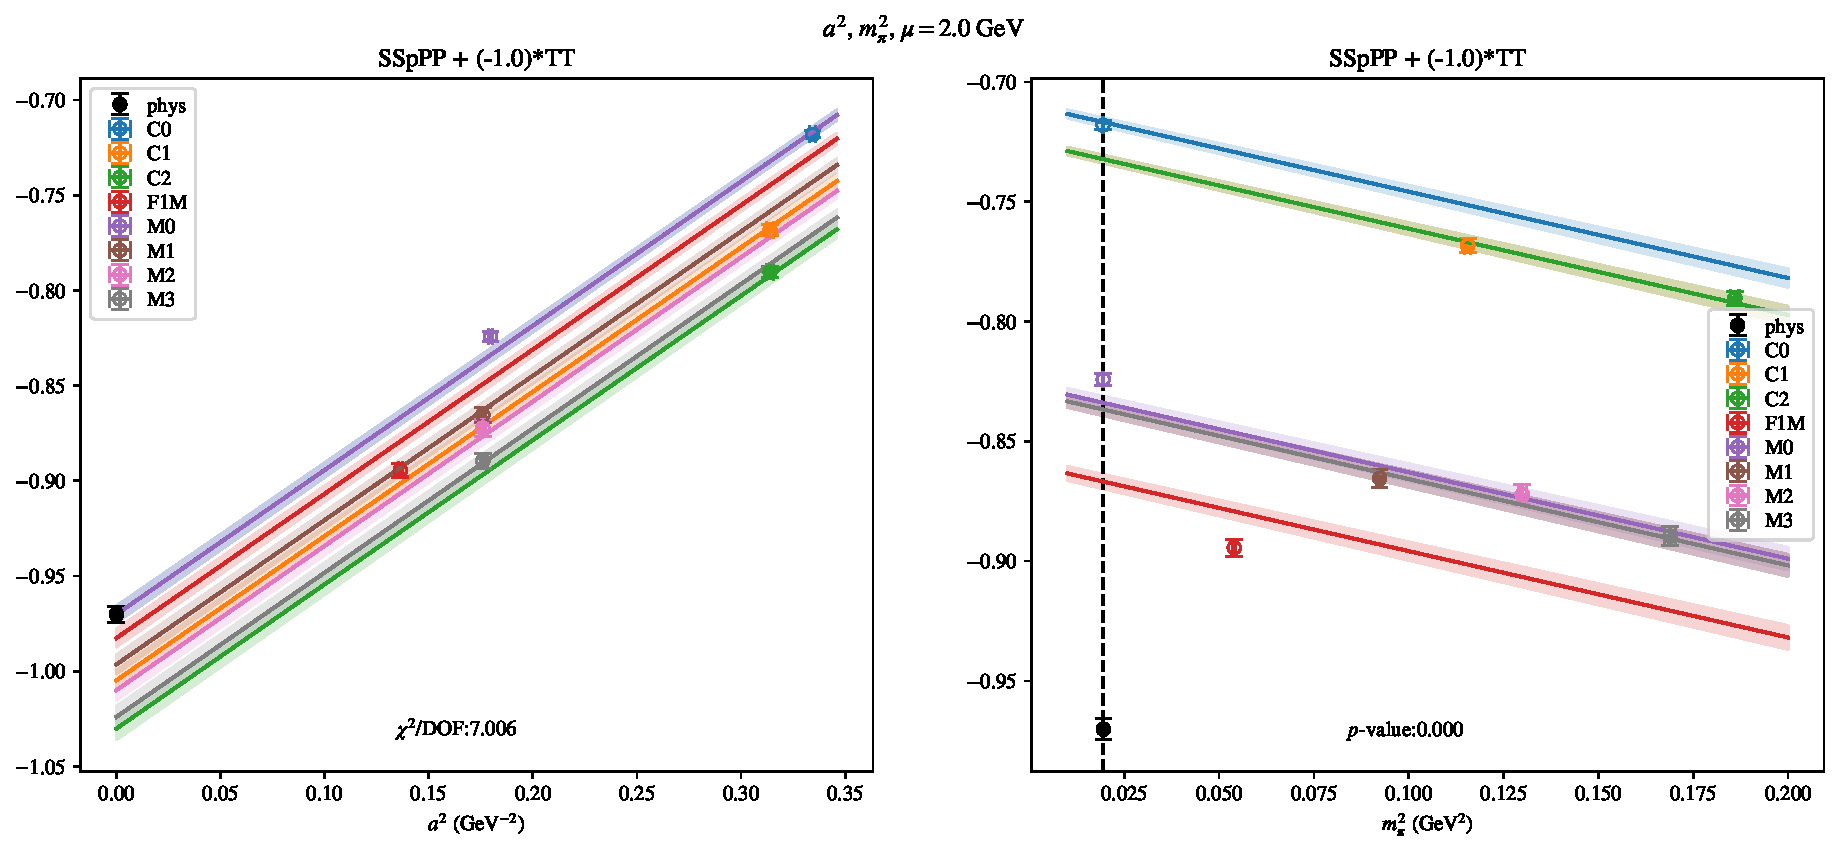
\includepdf[link, pages=-]{VVmAA/SUSY_F/a2m2_20.pdf}
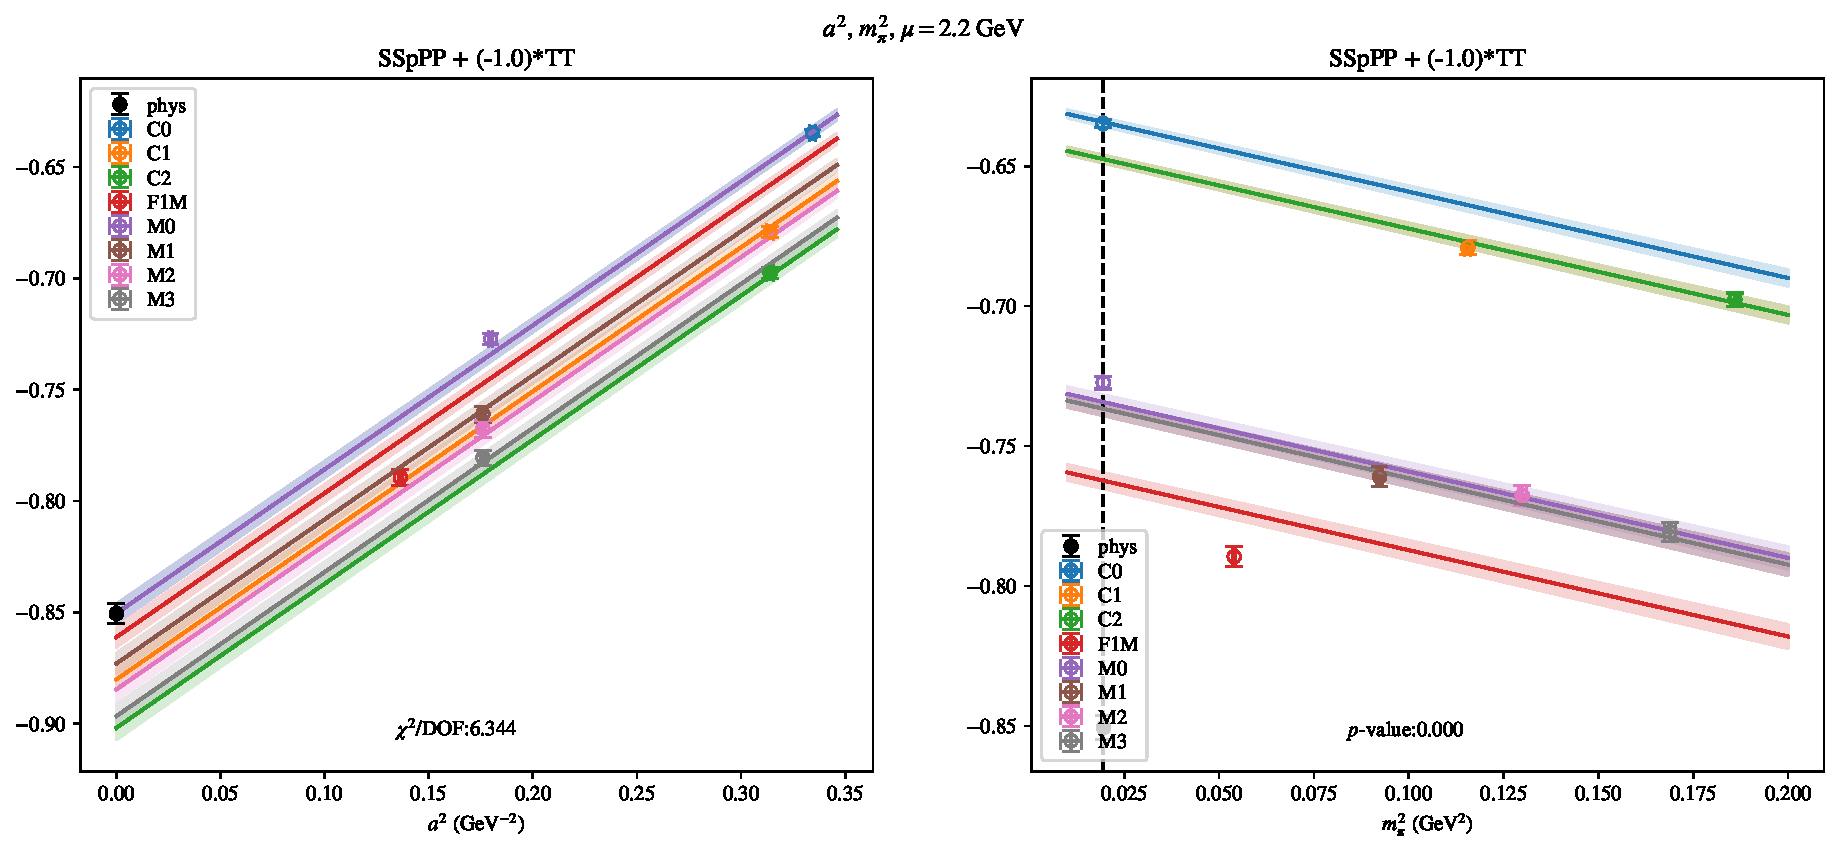
\includepdf[link, pages=-]{VVmAA/SUSY_F/a2m2_22.pdf}
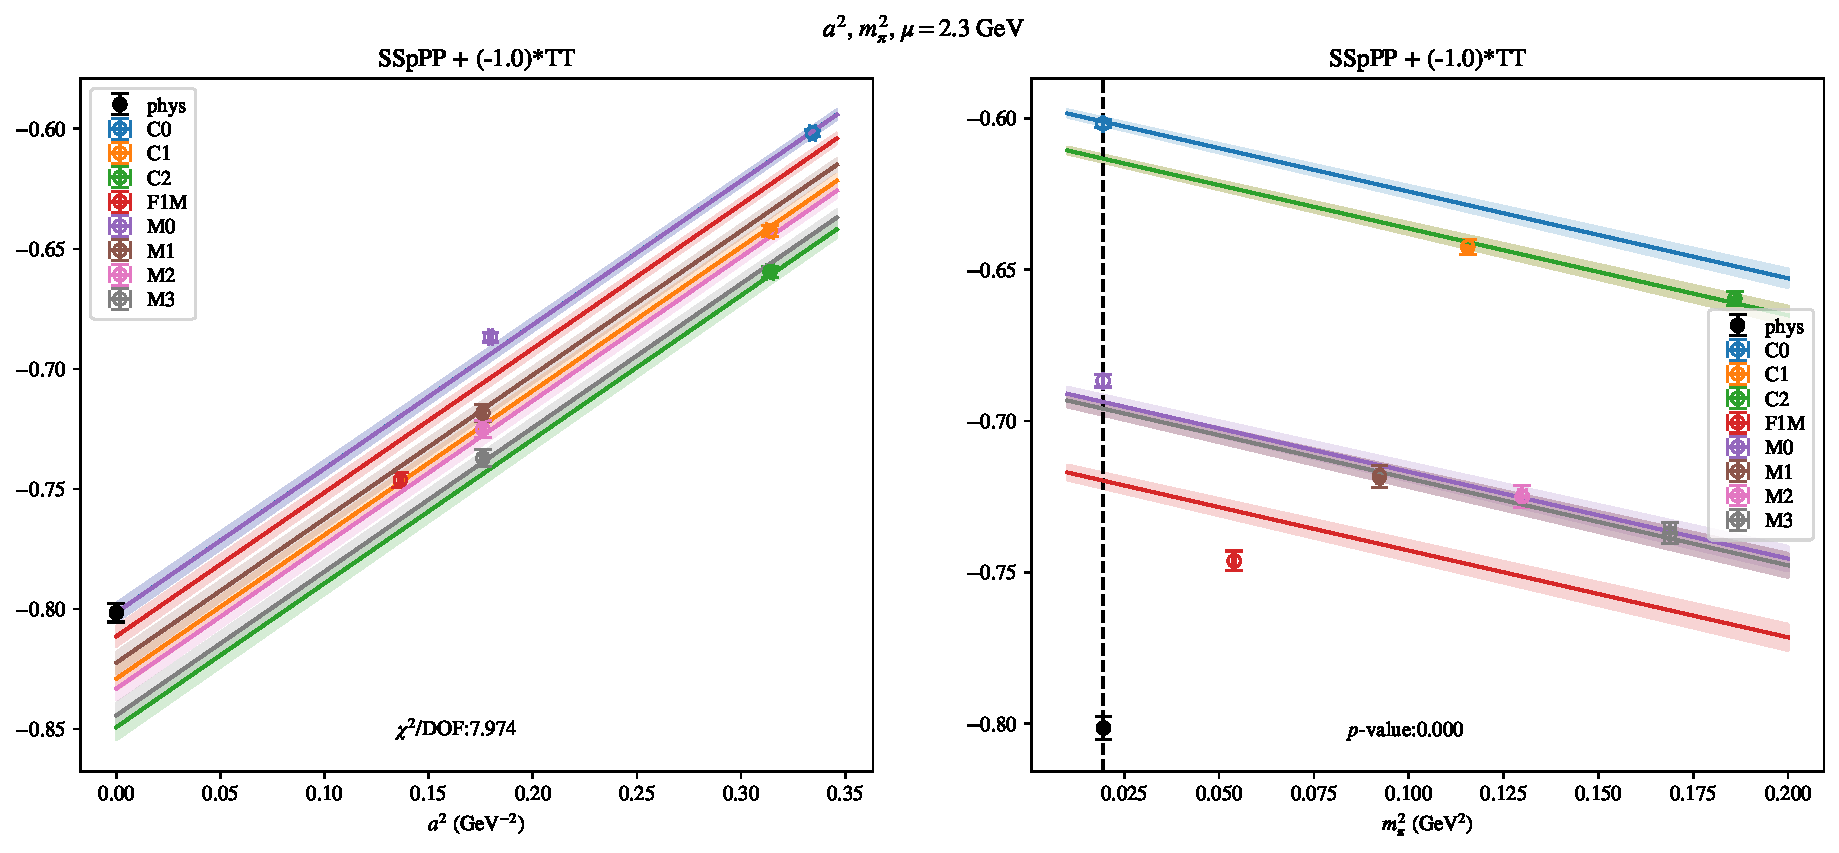
\includepdf[link, pages=-]{VVmAA/SUSY_F/a2m2_23.pdf}
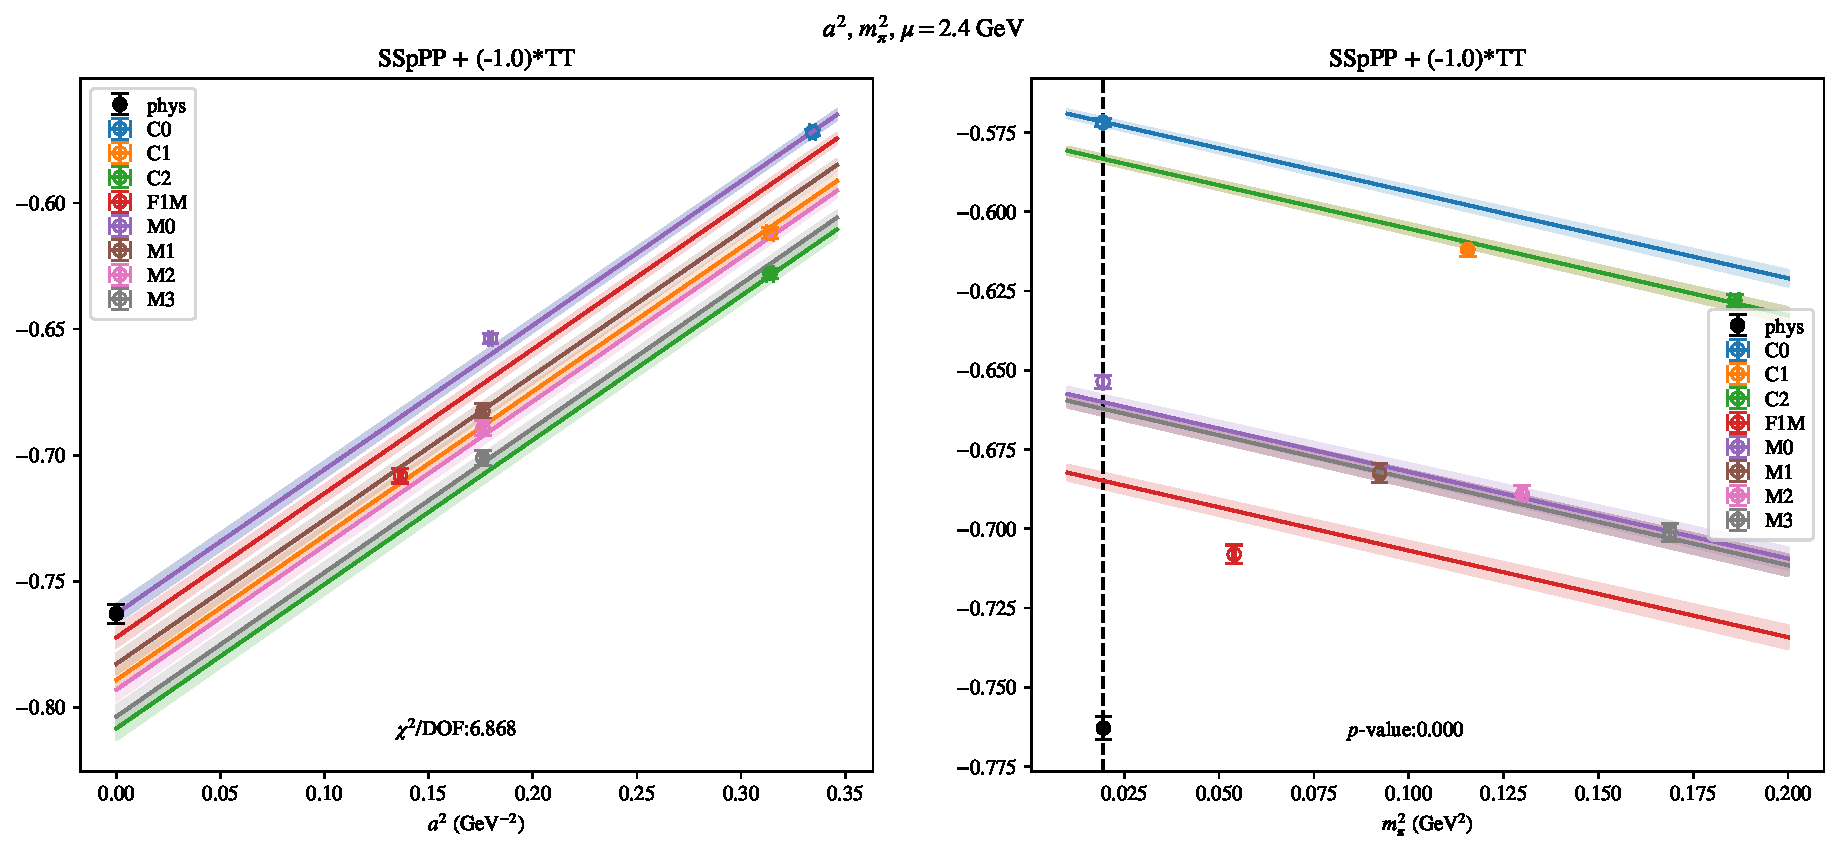
\includepdf[link, pages=-]{VVmAA/SUSY_F/a2m2_24.pdf}
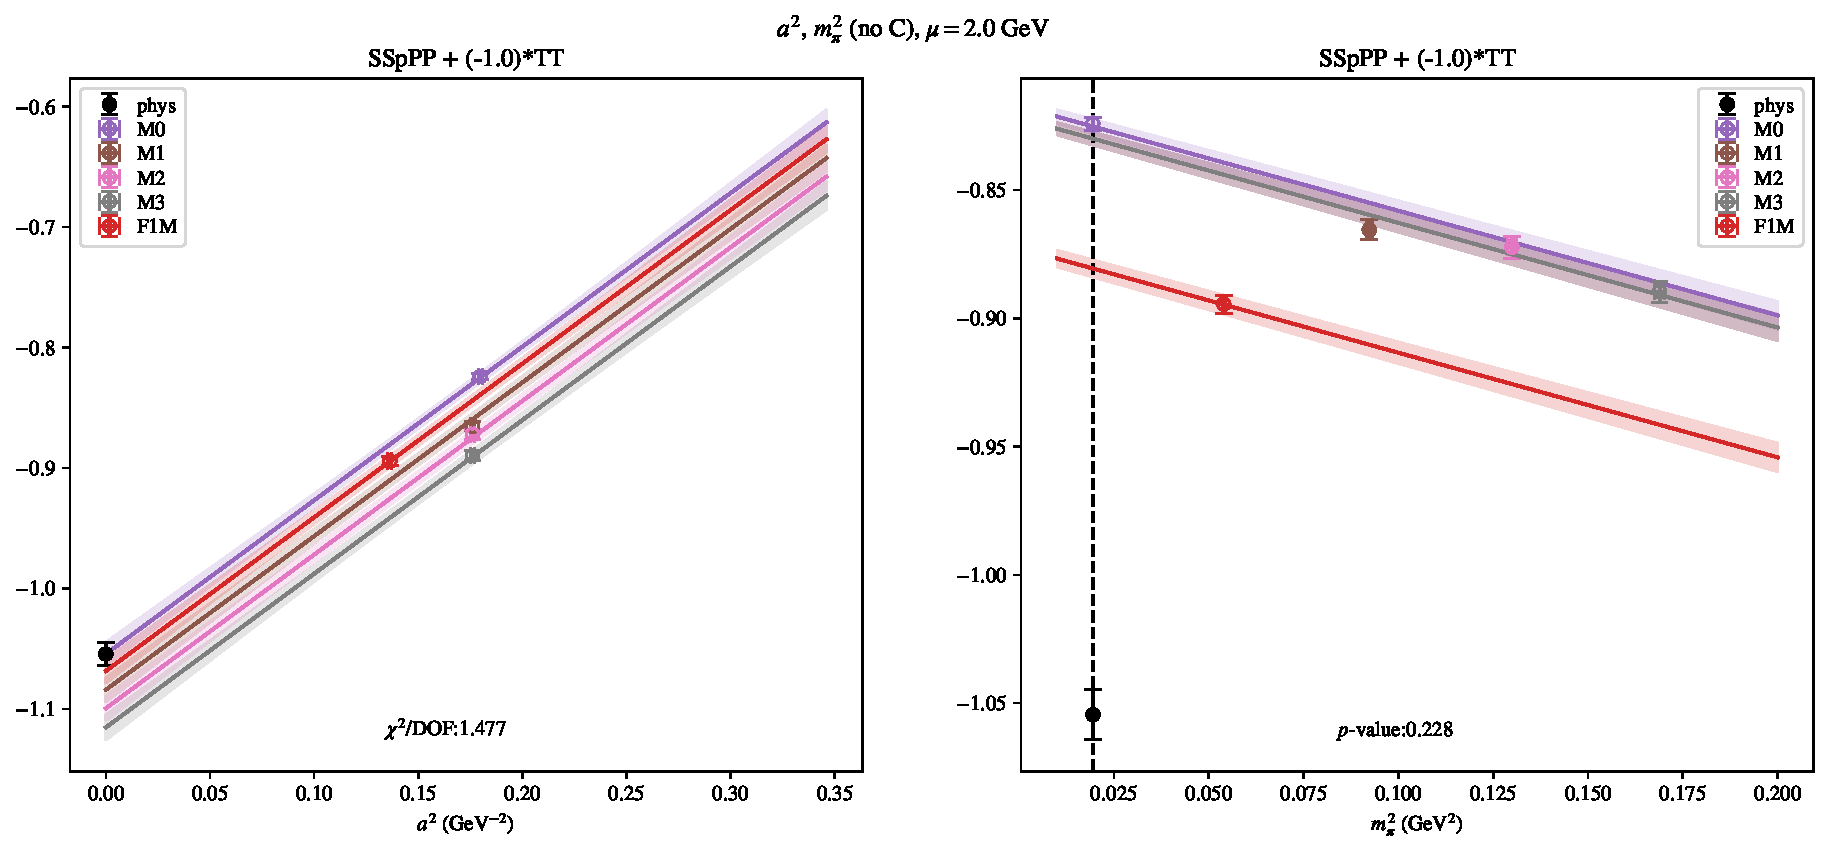
\includepdf[link, pages=-]{VVmAA/SUSY_F/a2m2noC_20.pdf}
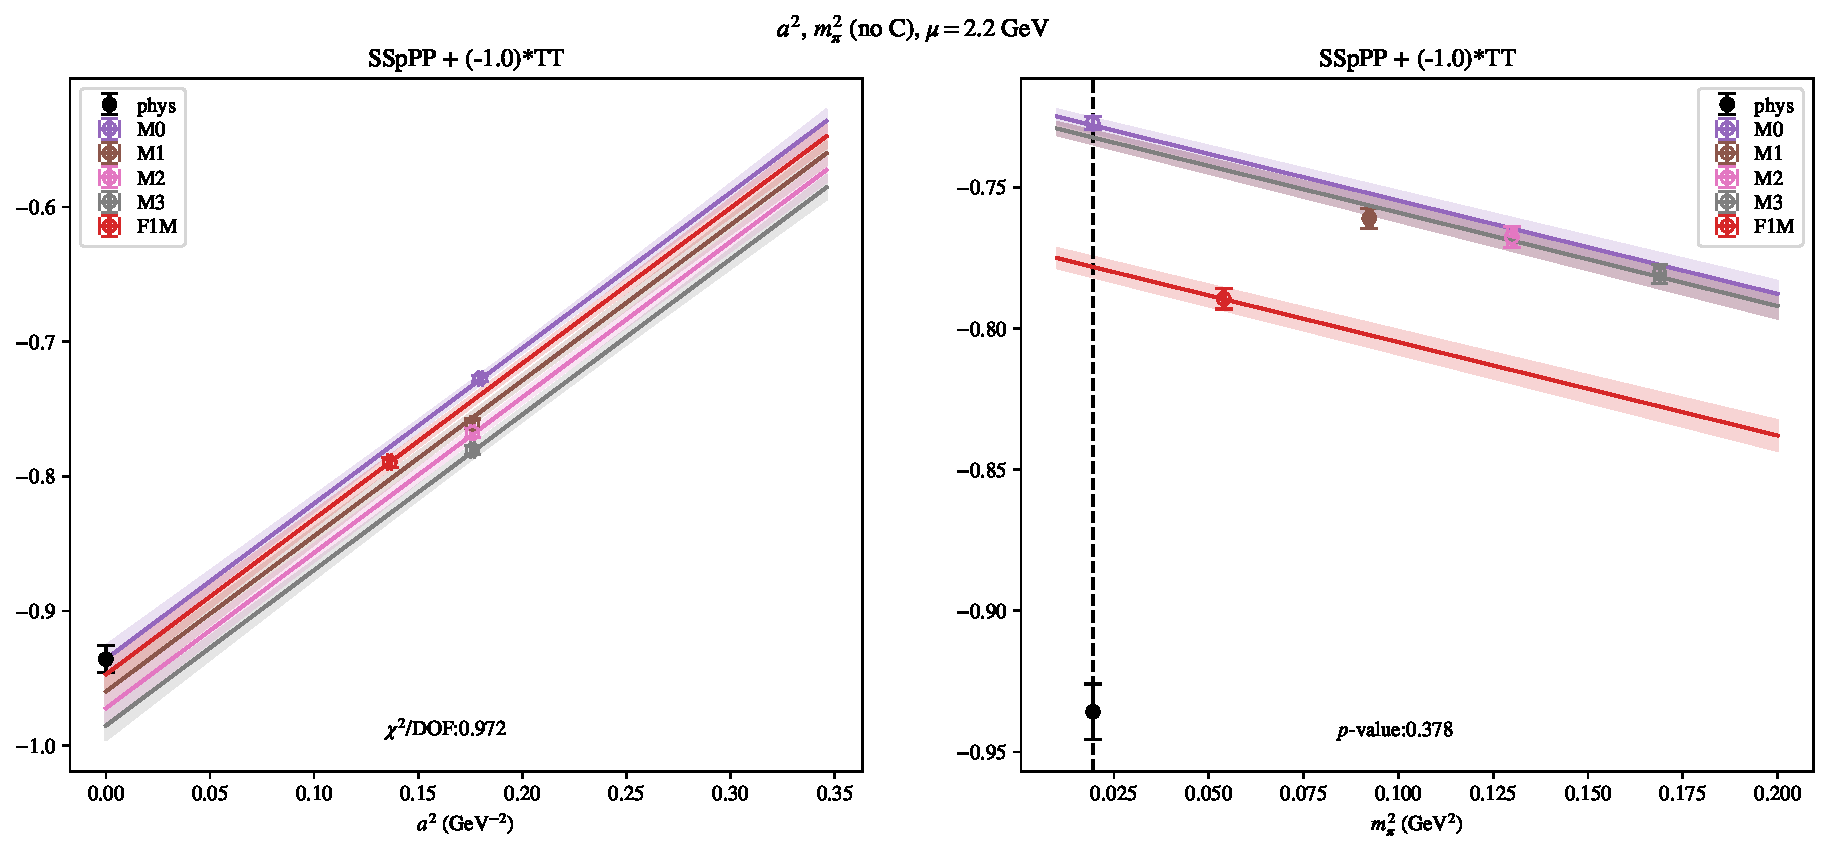
\includepdf[link, pages=-]{VVmAA/SUSY_F/a2m2noC_22.pdf}
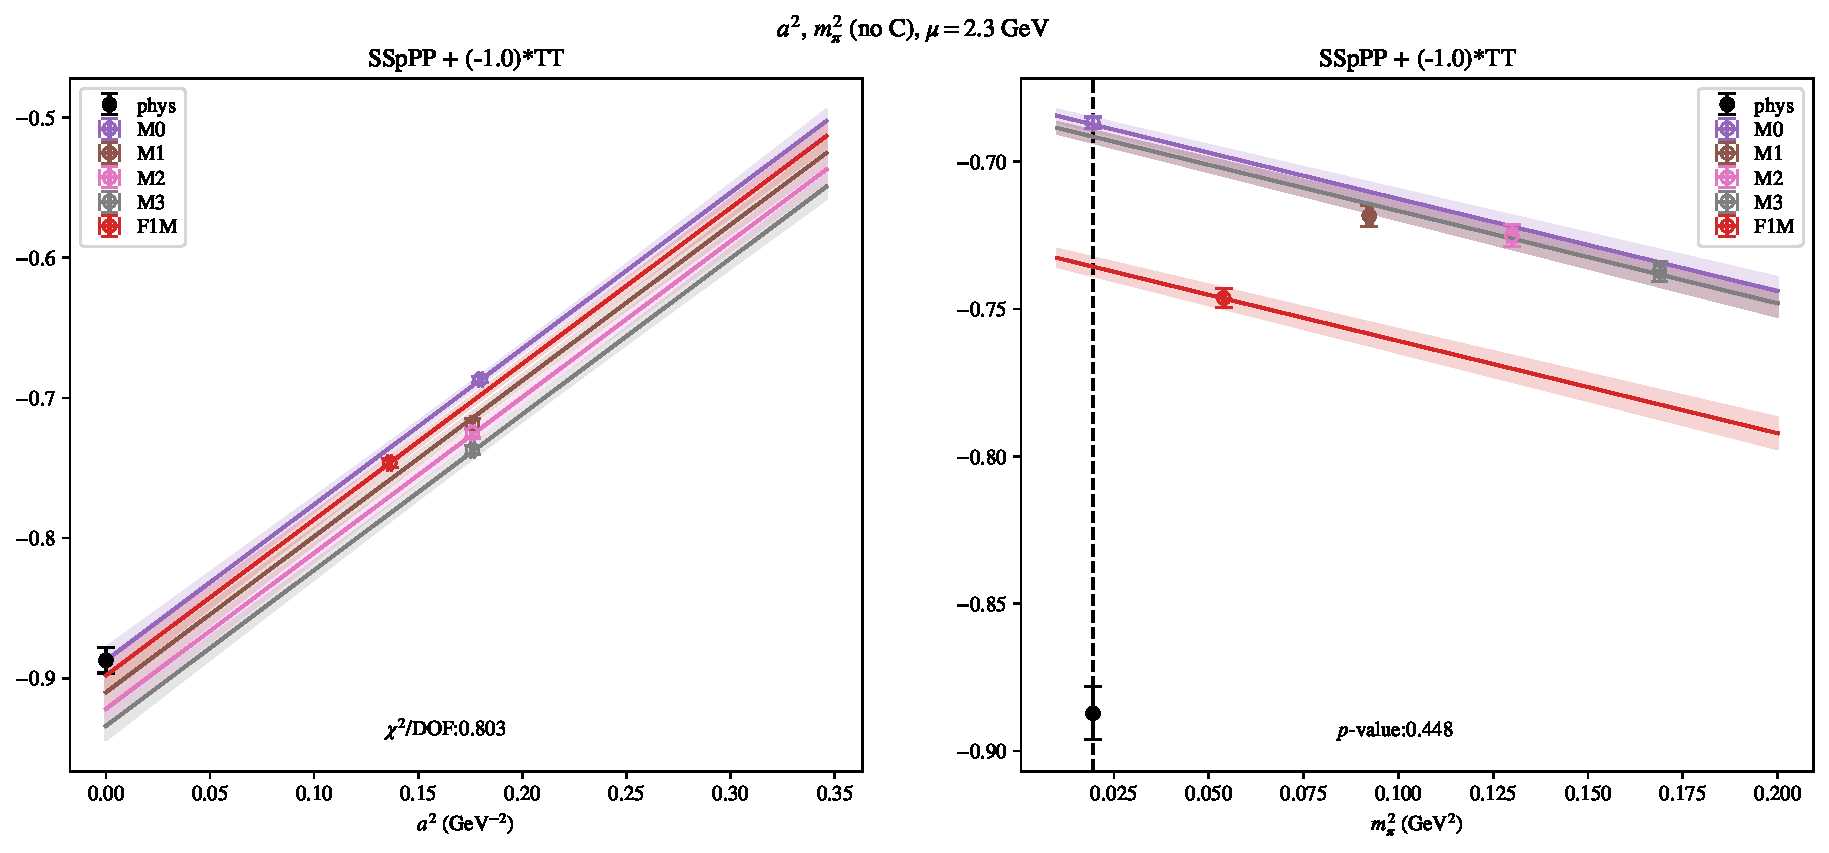
\includepdf[link, pages=-]{VVmAA/SUSY_F/a2m2noC_23.pdf}
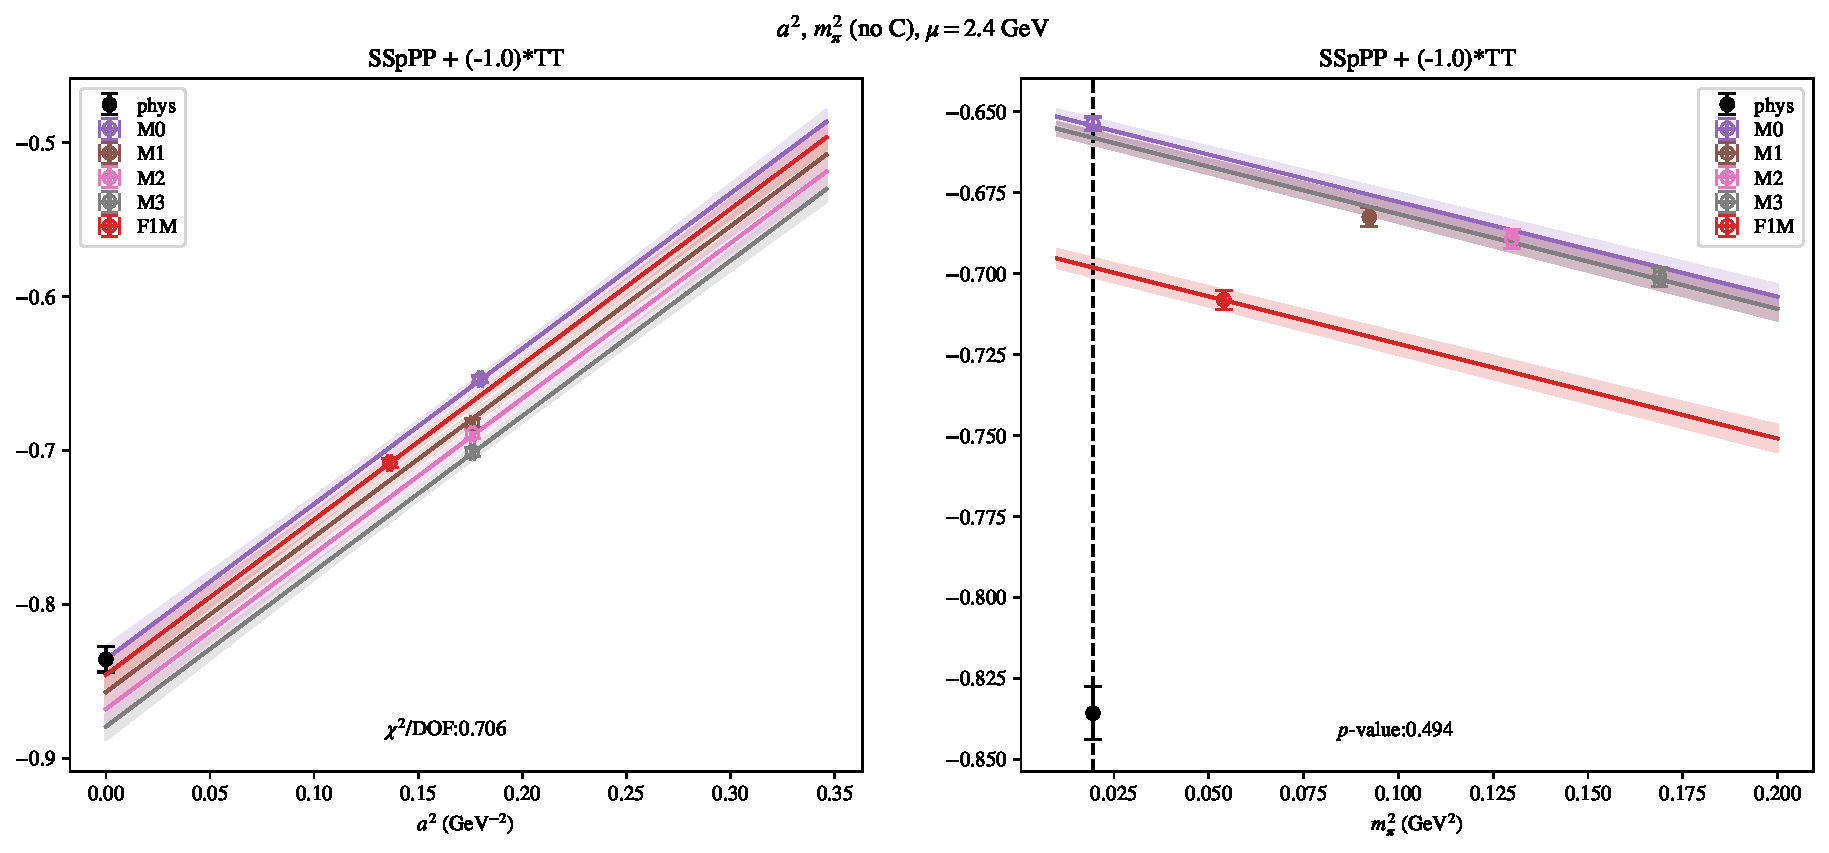
\includepdf[link, pages=-]{VVmAA/SUSY_F/a2m2noC_24.pdf}
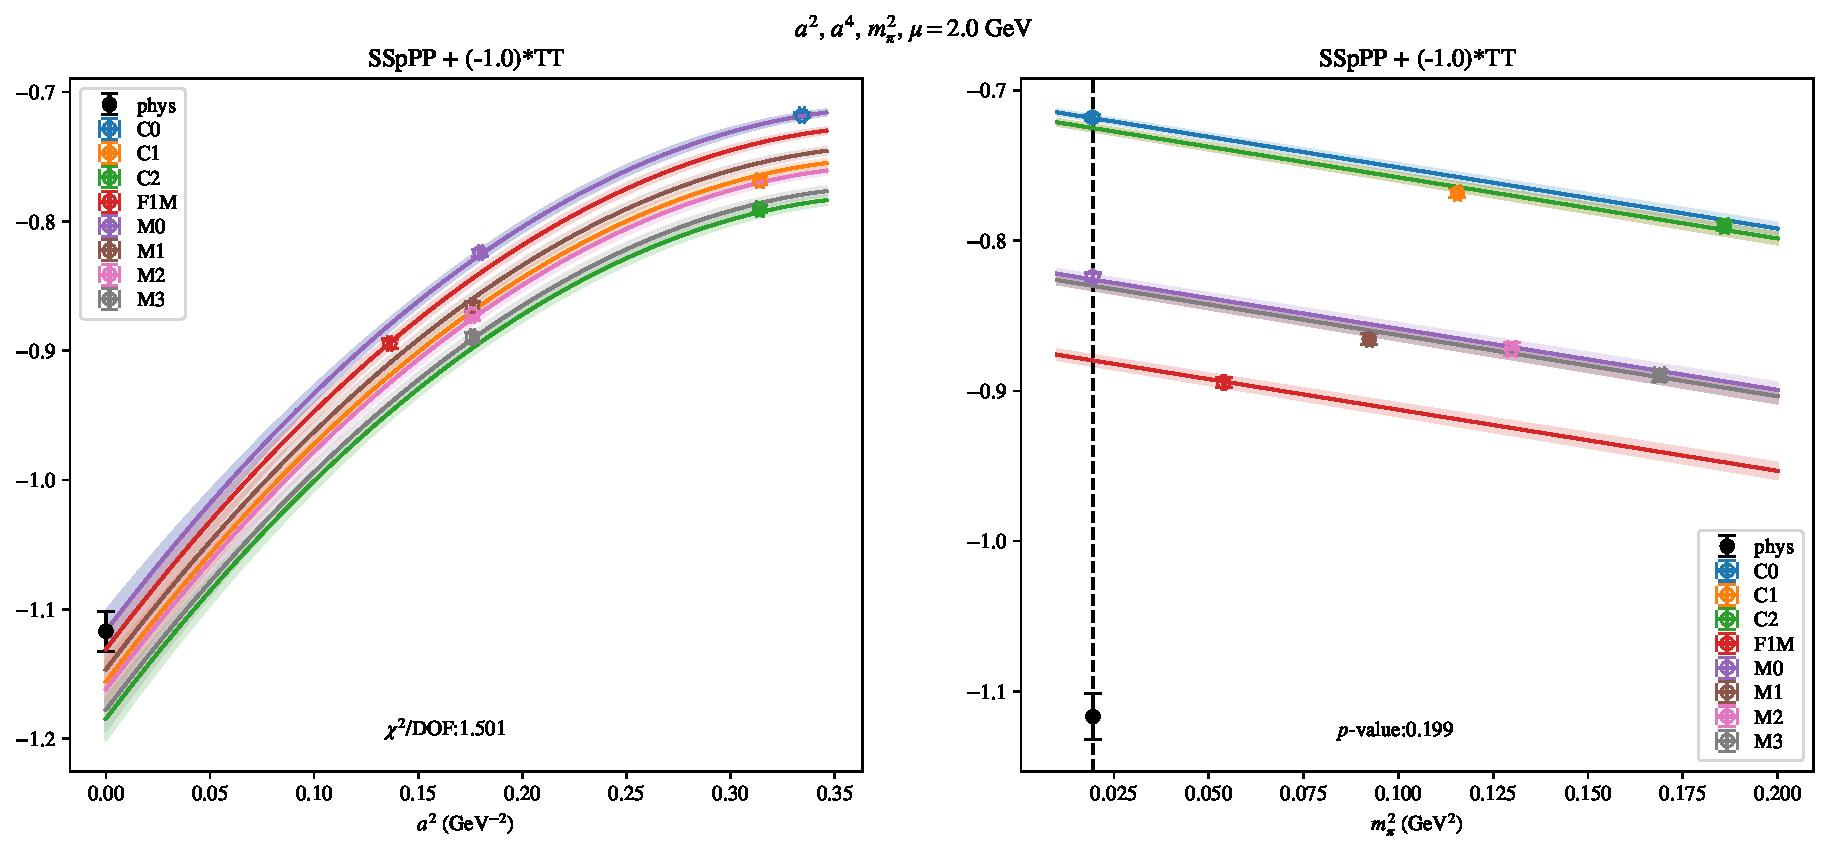
\includepdf[link, pages=-]{VVmAA/SUSY_F/a2a4m2_20.pdf}
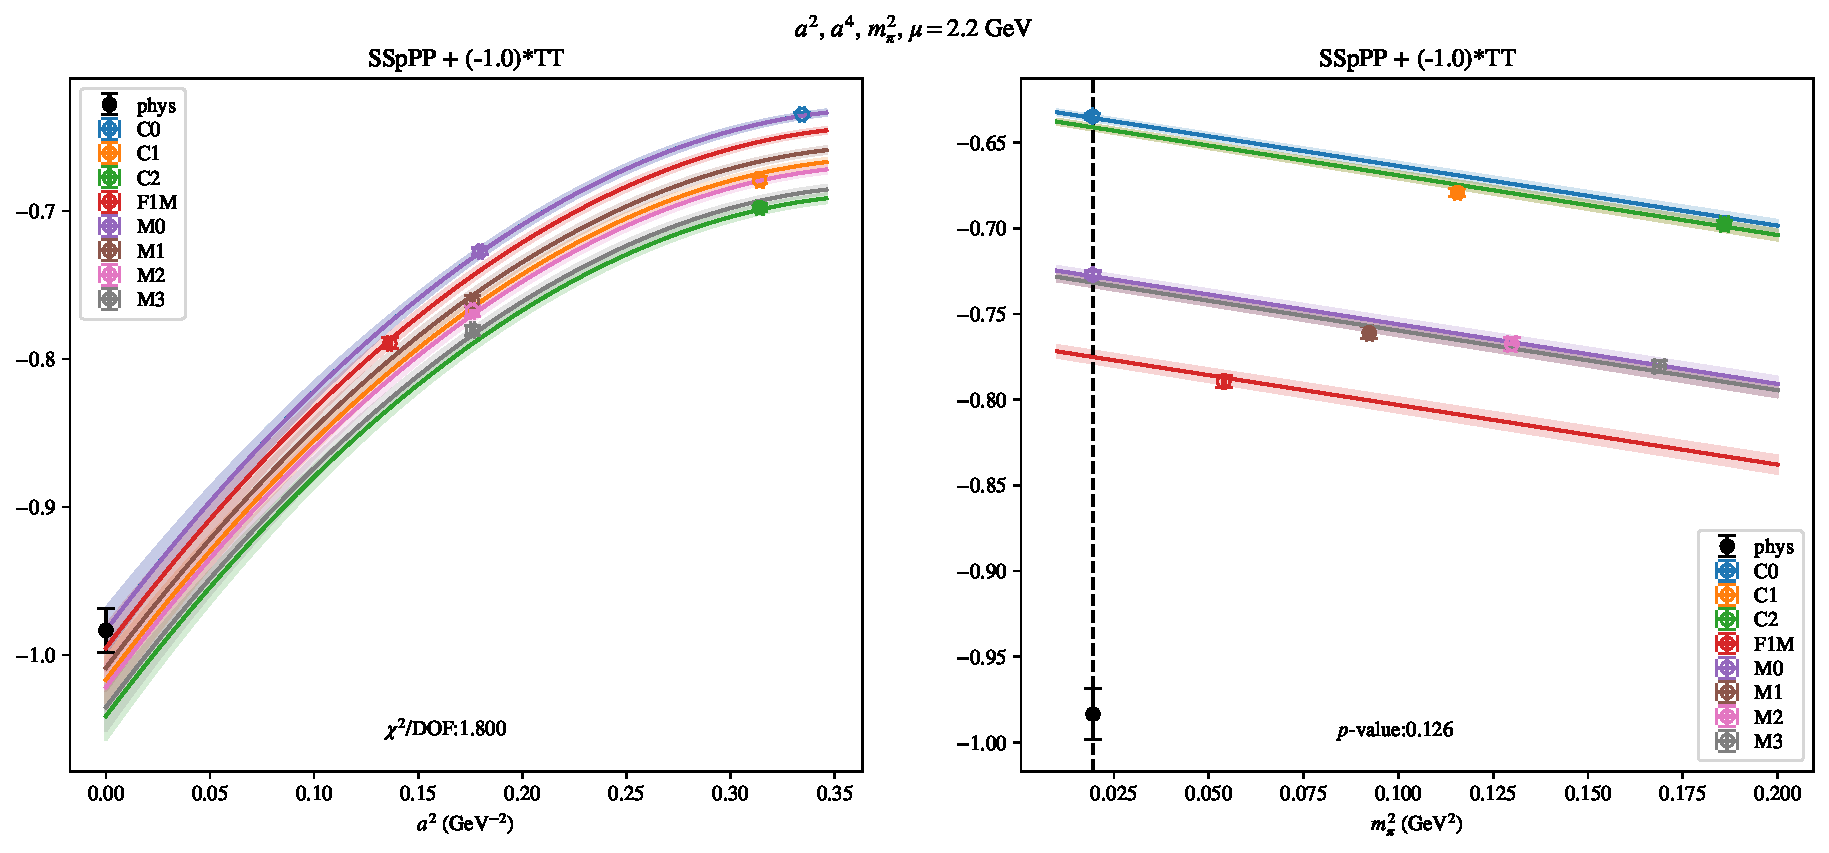
\includepdf[link, pages=-]{VVmAA/SUSY_F/a2a4m2_22.pdf}
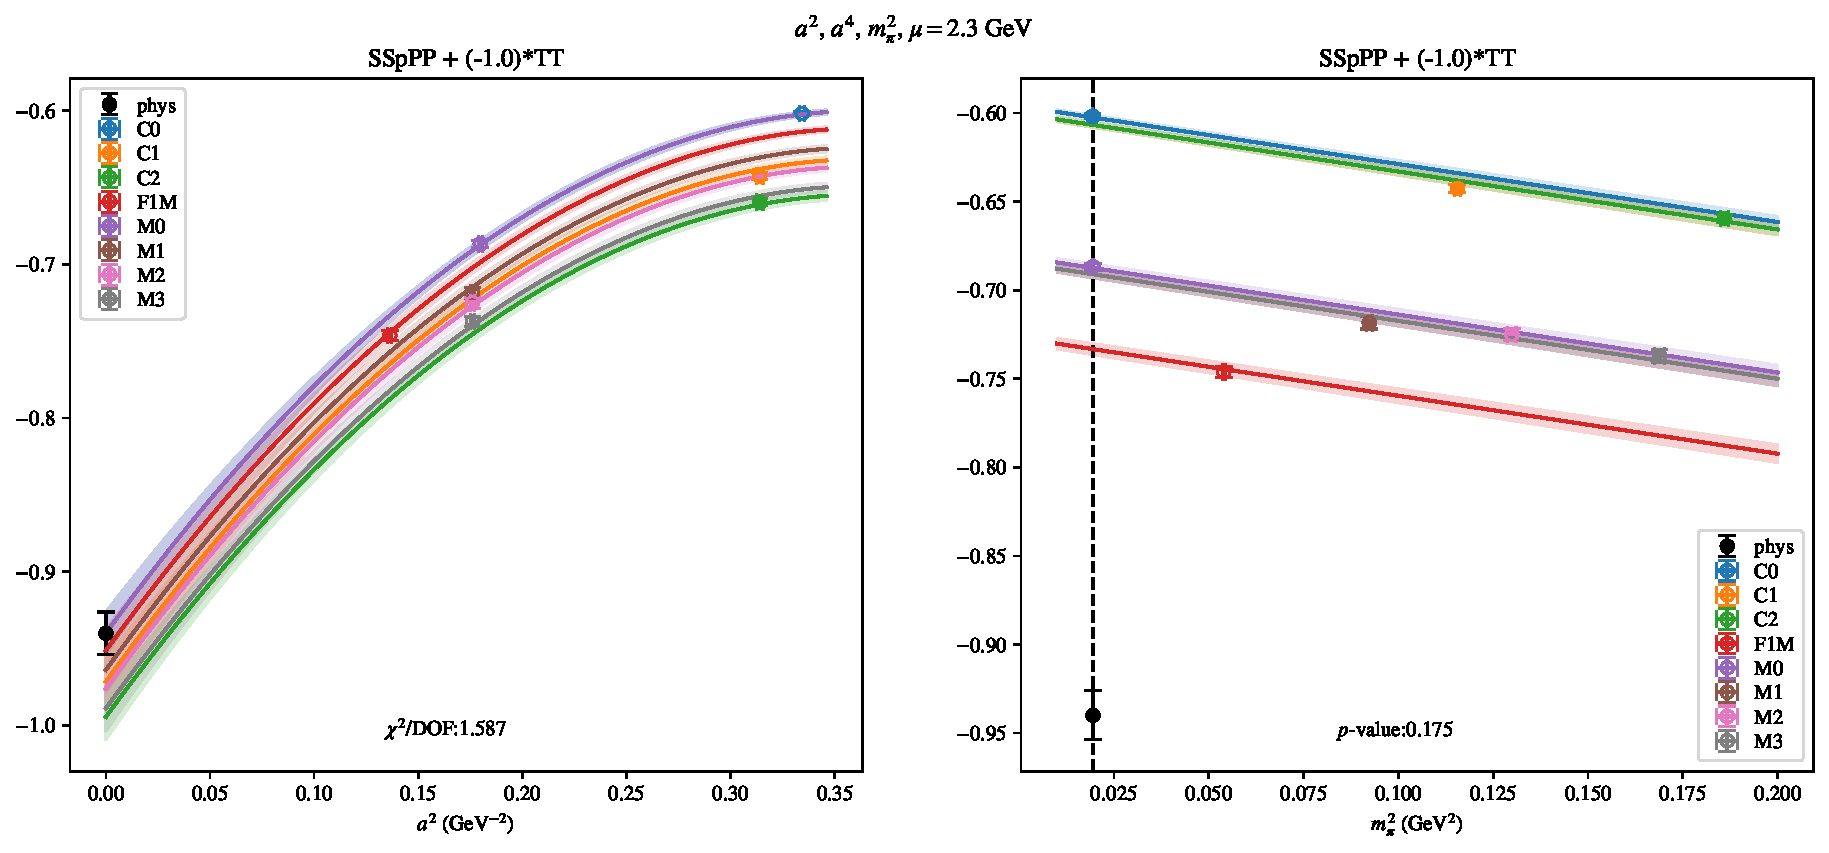
\includepdf[link, pages=-]{VVmAA/SUSY_F/a2a4m2_23.pdf}
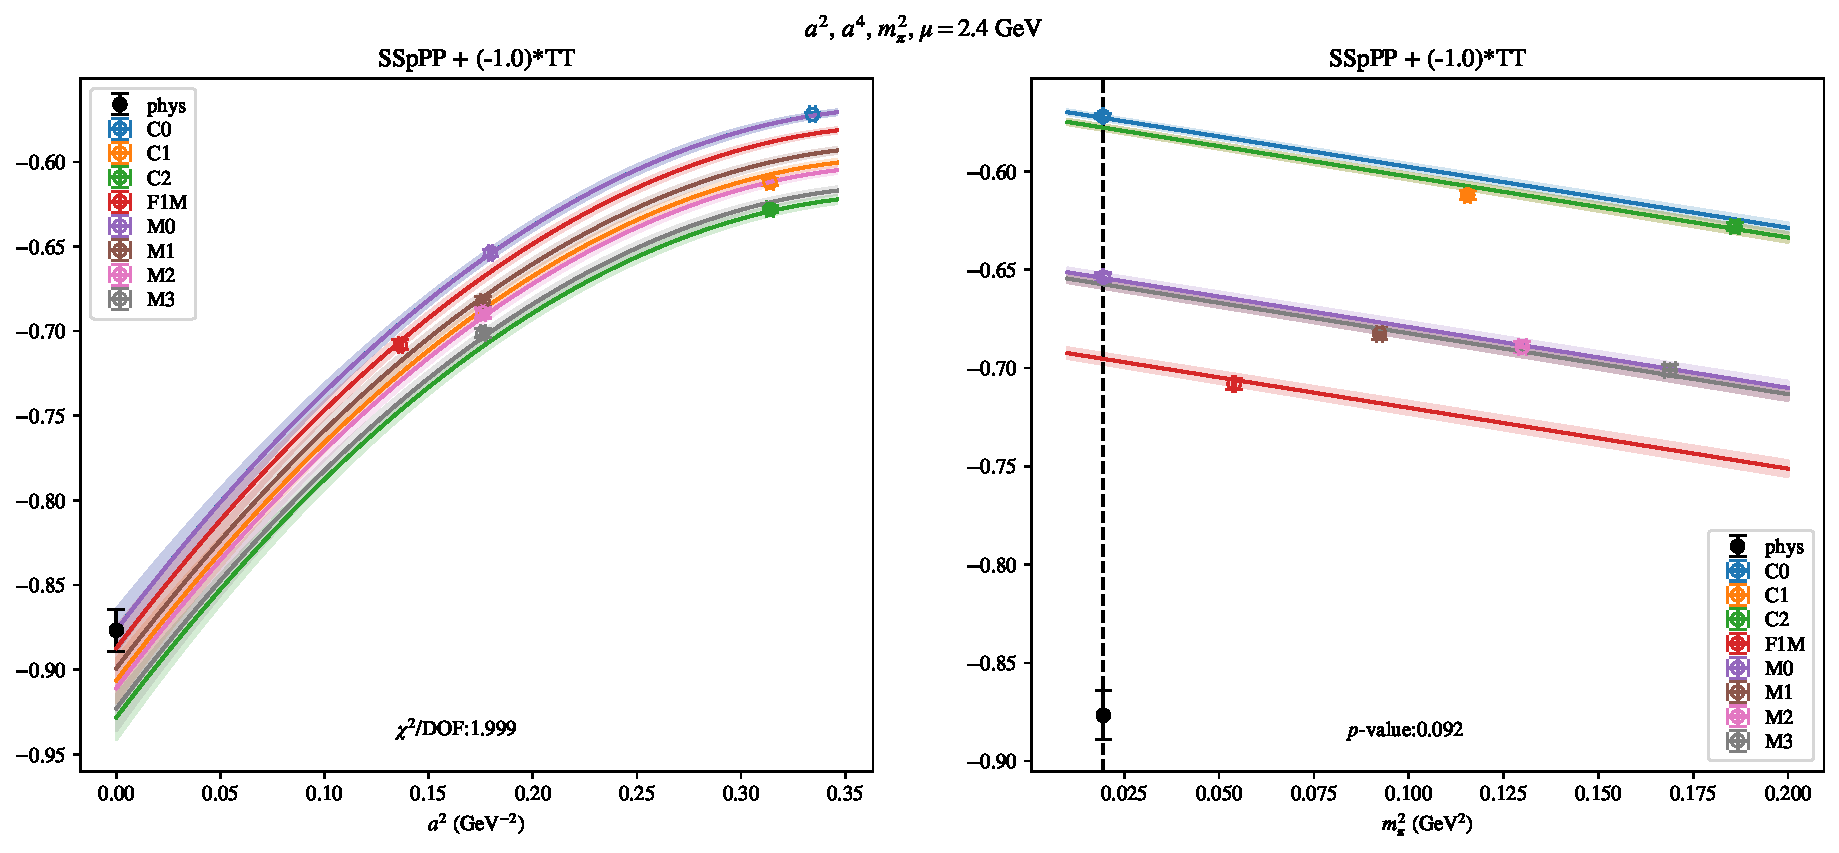
\includepdf[link, pages=-]{VVmAA/SUSY_F/a2a4m2_24.pdf}
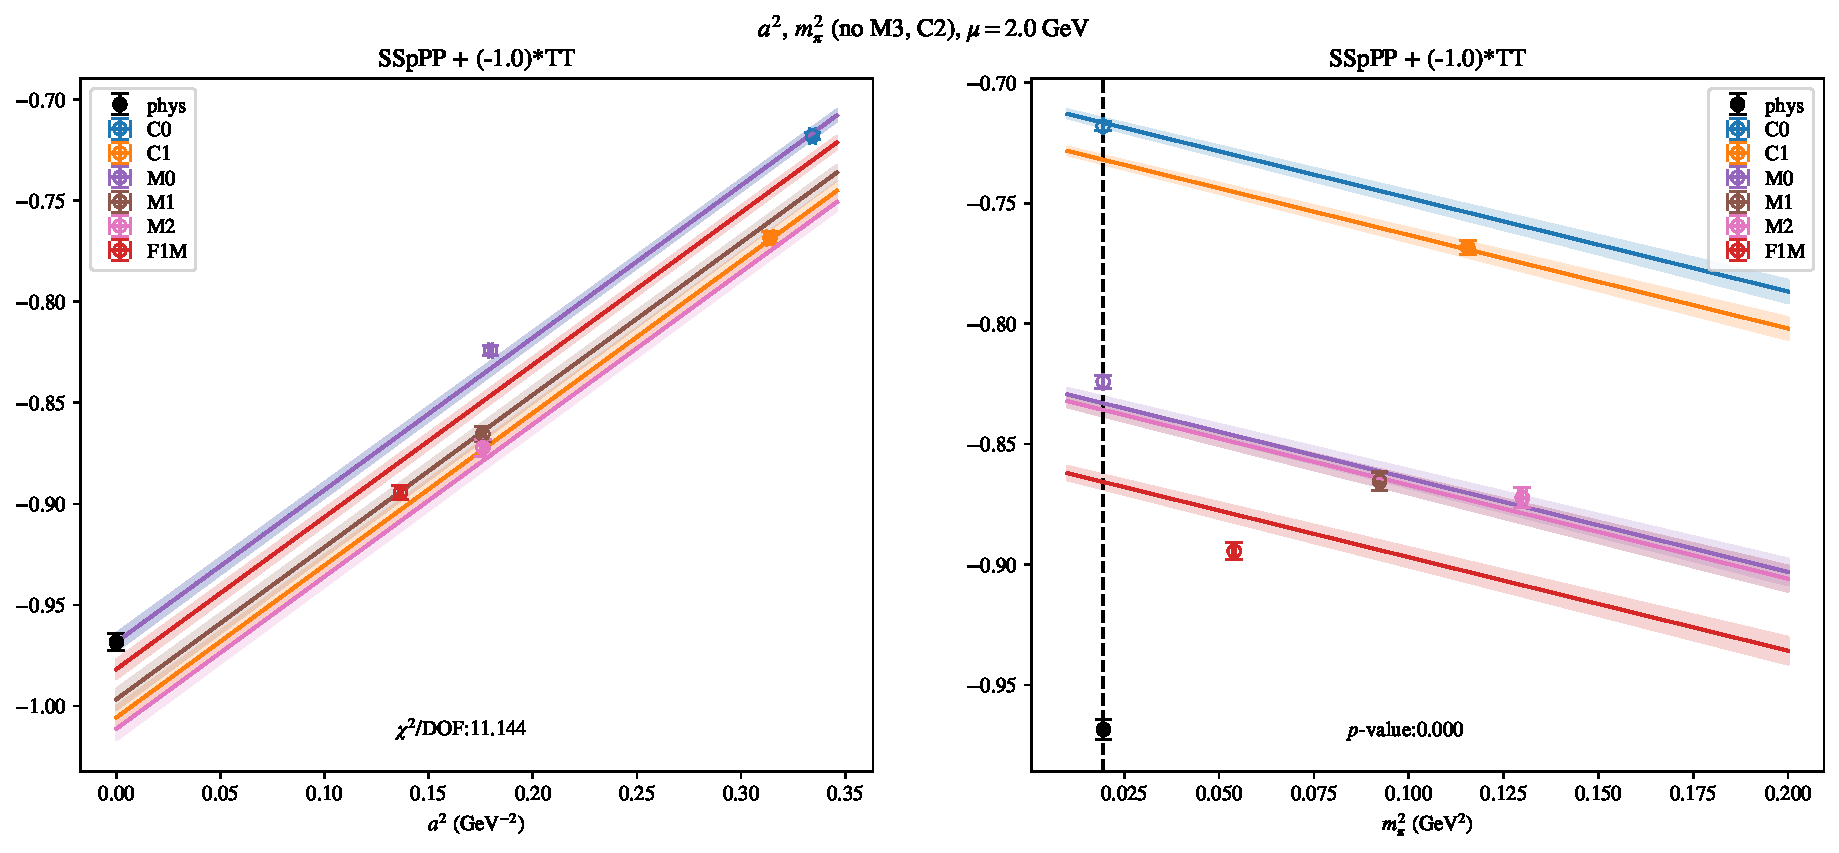
\includepdf[link, pages=-]{VVmAA/SUSY_F/a2m2mcut_20.pdf}
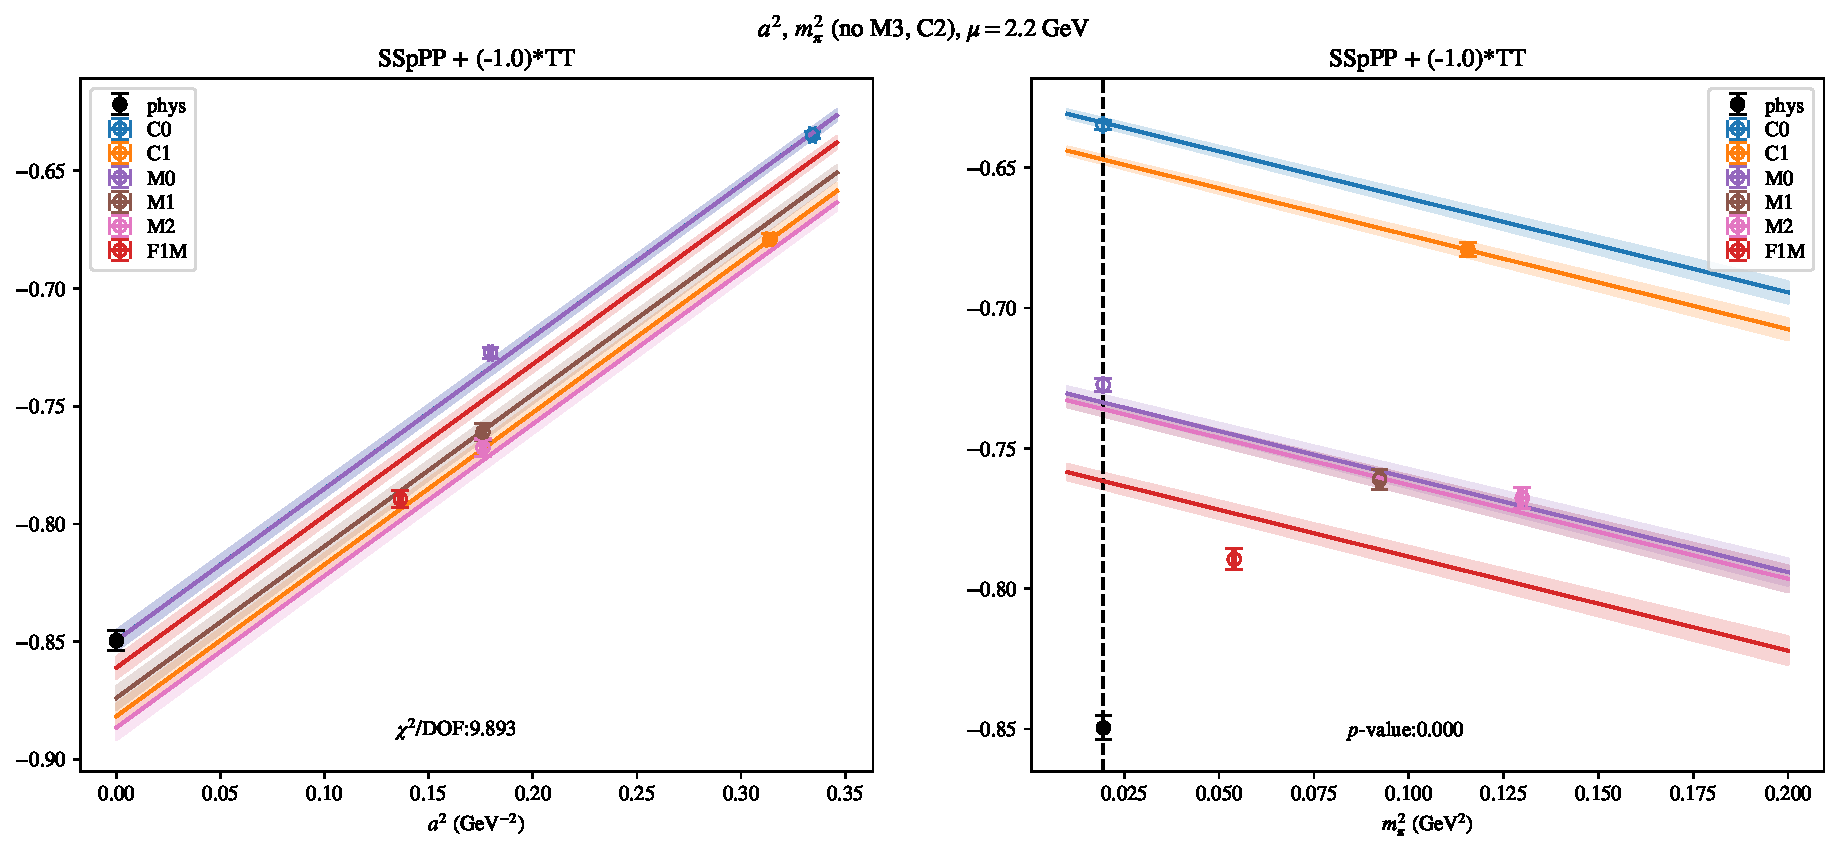
\includepdf[link, pages=-]{VVmAA/SUSY_F/a2m2mcut_22.pdf}
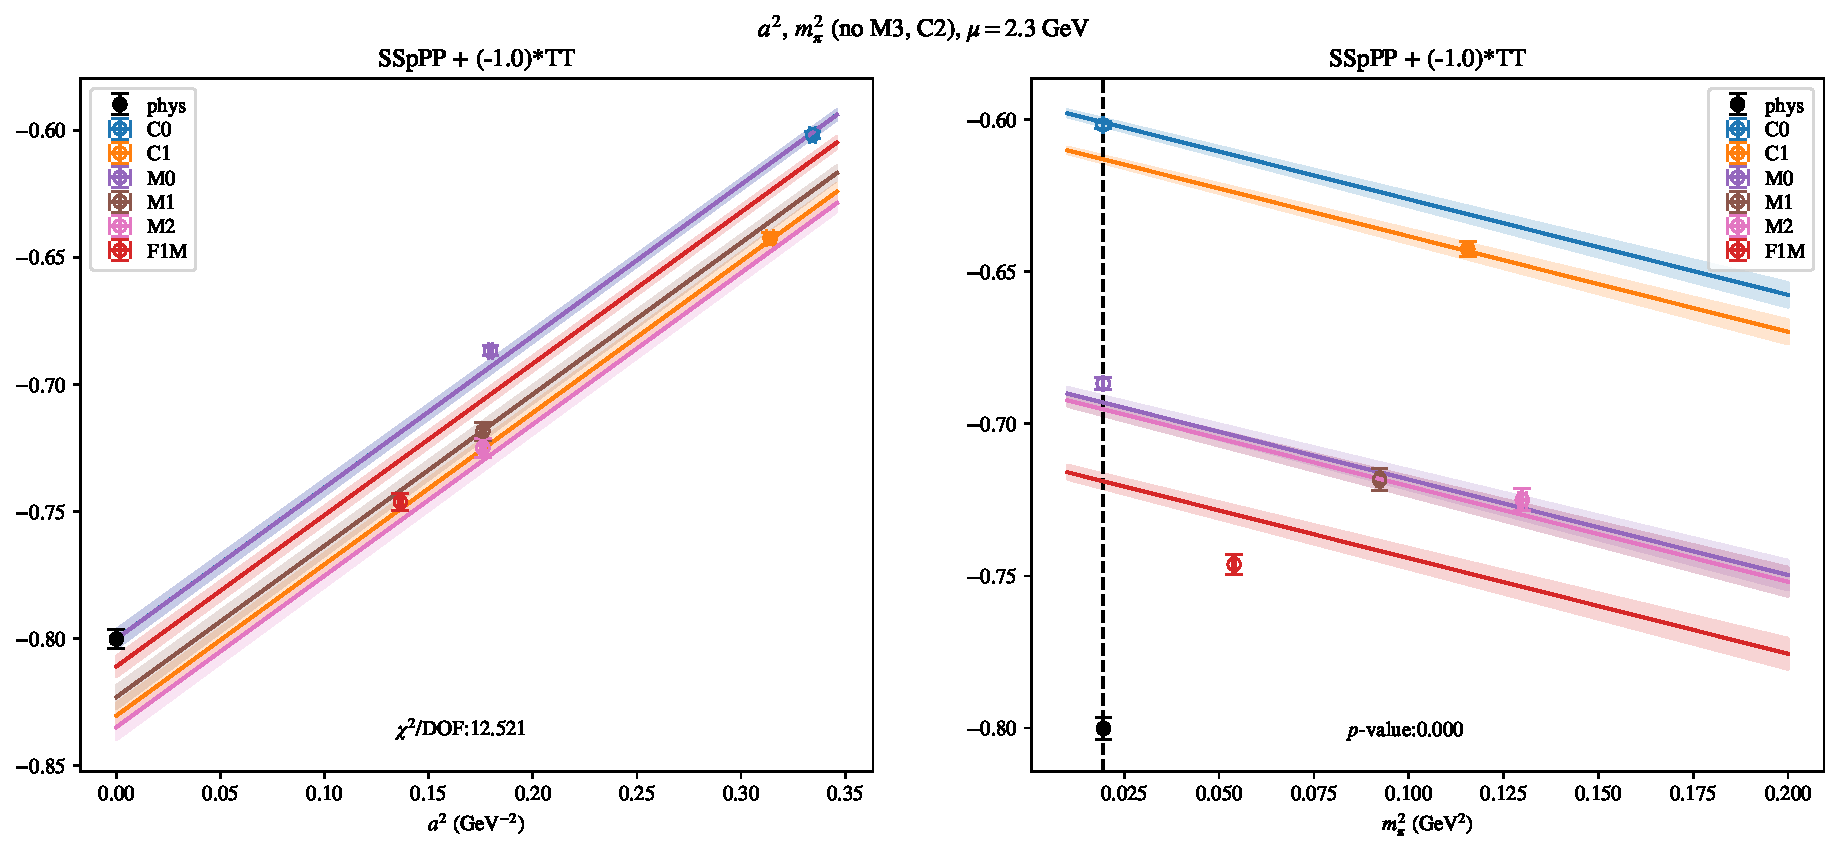
\includepdf[link, pages=-]{VVmAA/SUSY_F/a2m2mcut_23.pdf}
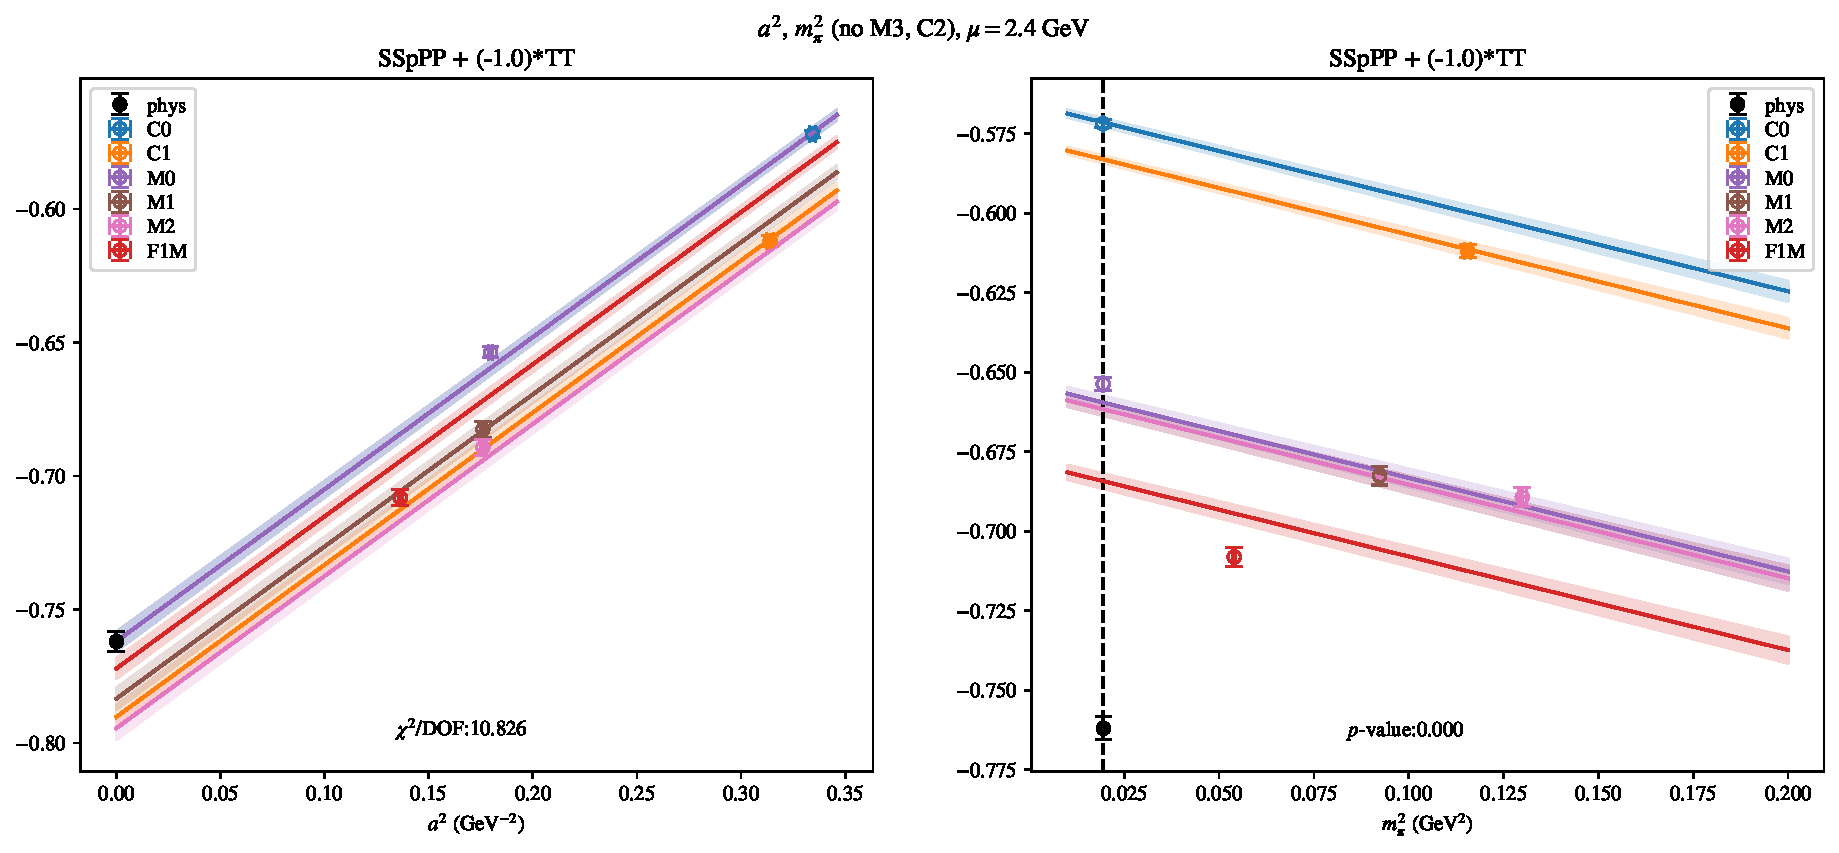
\includepdf[link, pages=-]{VVmAA/SUSY_F/a2m2mcut_24.pdf}
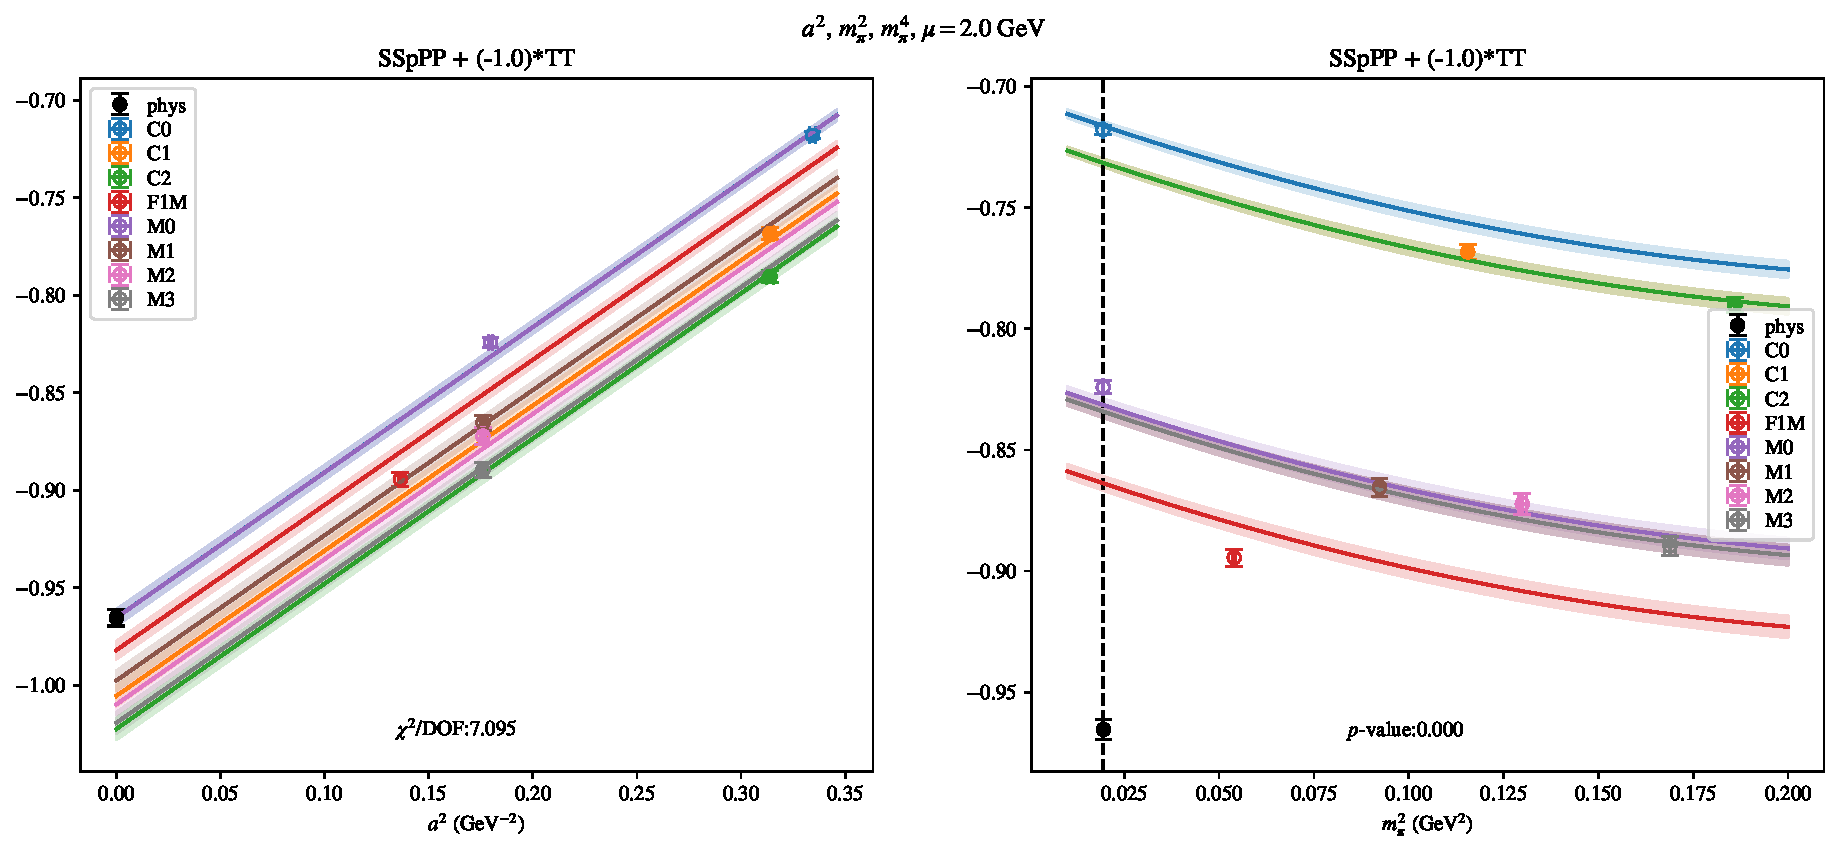
\includepdf[link, pages=-]{VVmAA/SUSY_F/a2m2m4_20.pdf}
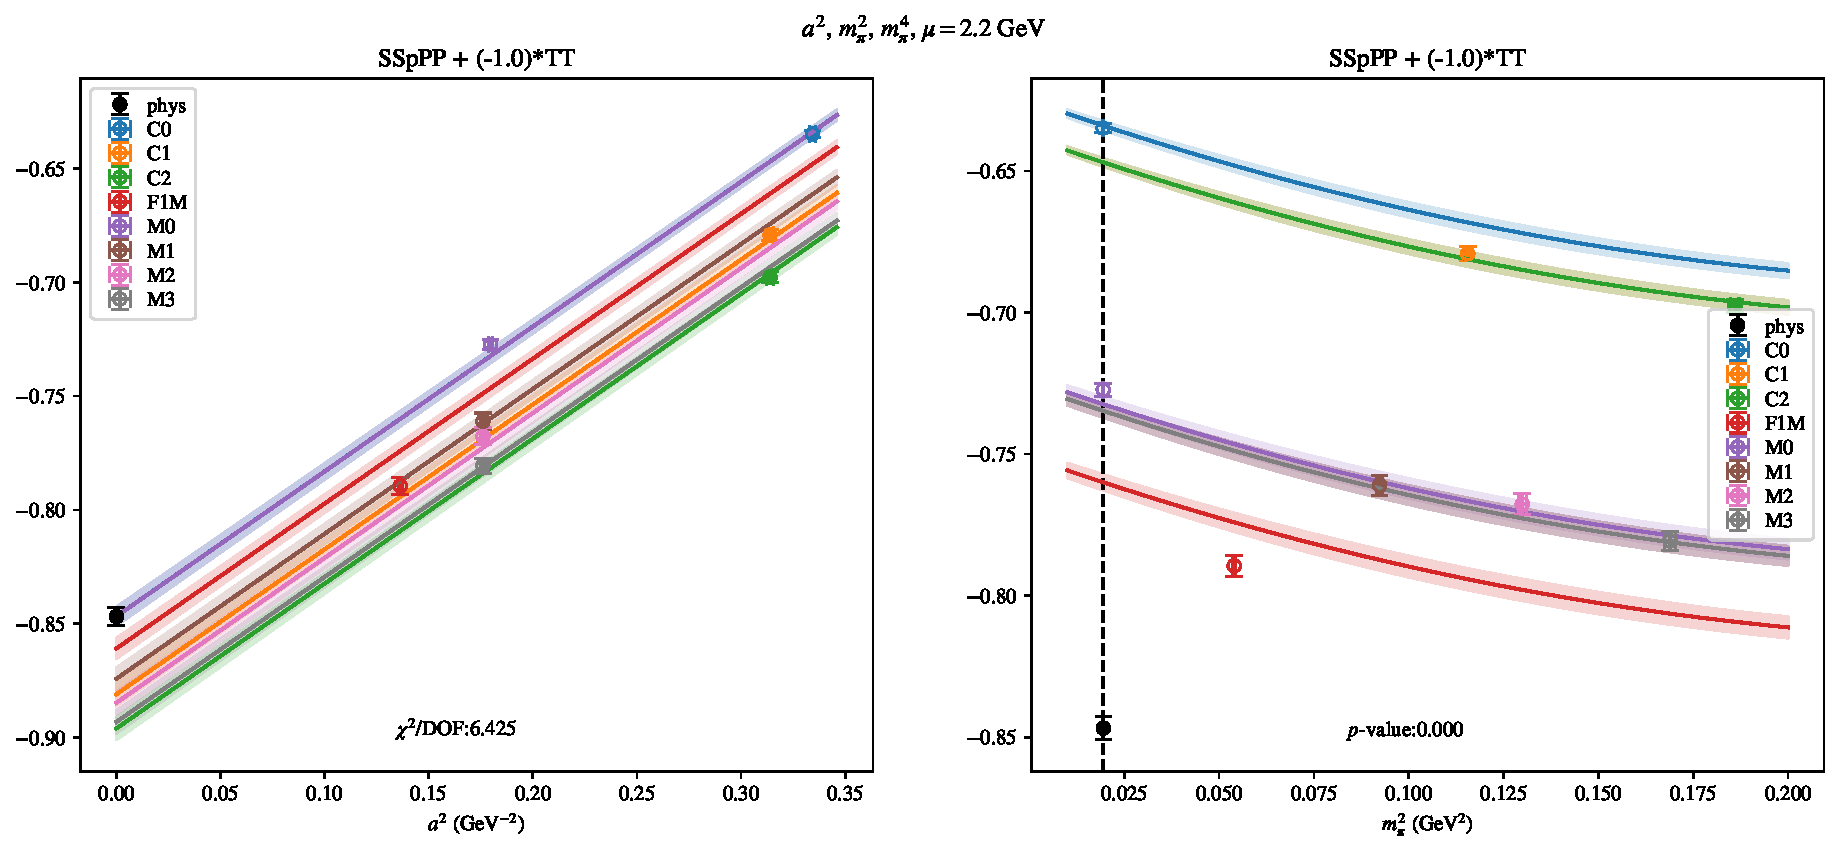
\includepdf[link, pages=-]{VVmAA/SUSY_F/a2m2m4_22.pdf}
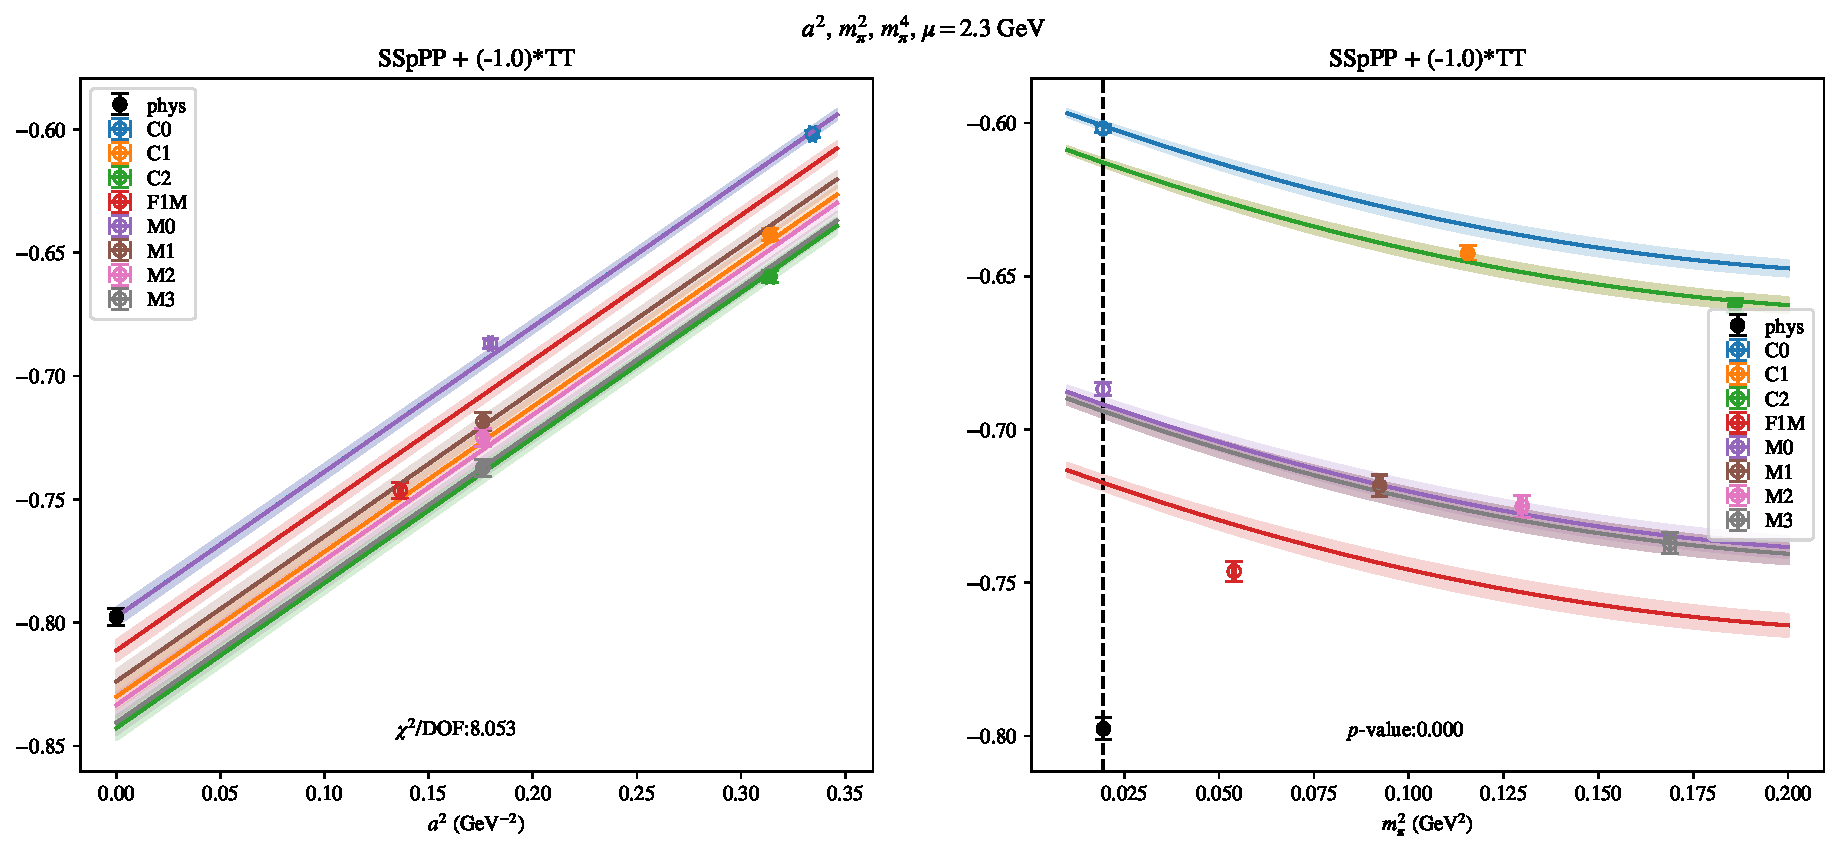
\includepdf[link, pages=-]{VVmAA/SUSY_F/a2m2m4_23.pdf}
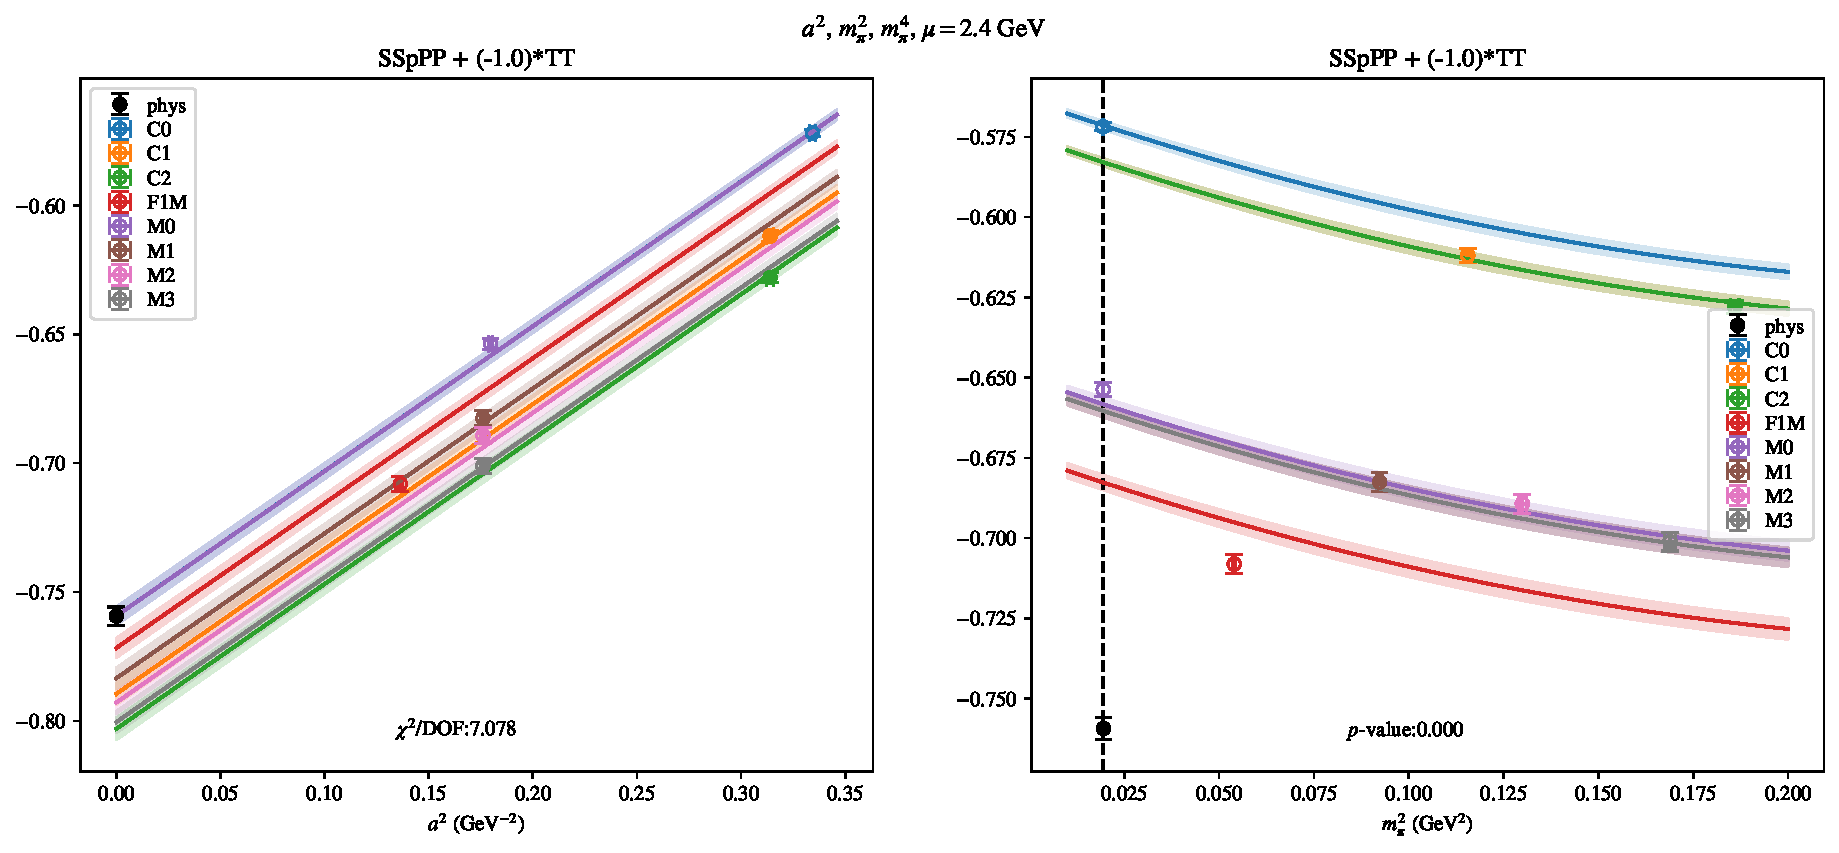
\includepdf[link, pages=-]{VVmAA/SUSY_F/a2m2m4_24.pdf}
\clearpage
\section{$B_3$}
\begin{table}[h!]
\begin{center}
\begin{tabular}{|c|c|c|c|c|c|}
\hline
$\mu$ (GeV) & $a^2$, $m_\pi^2$& $a^2$, $m_\pi^2$ (no C)& $a^2$, $a^4$, $m_\pi^2$& $a^2$, $m_\pi^2$ (no M3, C2)& $a^2$, $m_\pi^2$, $m_\pi^4$\\
\hline
2.0& \hyperlink{SSmPP/SUSY_F/a2m2_20.pdf.1}{\textbf{-0.2835(47)}: 5.155 (0.0)} & \hyperlink{SSmPP/SUSY_F/a2m2noC_20.pdf.1}{\textbf{-0.295(27)}: 0.934 (0.393)} & \hyperlink{SSmPP/SUSY_F/a2a4m2_20.pdf.1}{\textbf{-0.299(43)}: 3.111 (0.014)} & \hyperlink{SSmPP/SUSY_F/a2m2mcut_20.pdf.1}{\textbf{-0.2834(50)}: 7.311 (0.0)} & \hyperlink{SSmPP/SUSY_F/a2m2m4_20.pdf.1}{\textbf{-0.2829(50)}: 4.514 (0.001)}\\
2.2& \hyperlink{SSmPP/SUSY_F/a2m2_22.pdf.1}{\textbf{-0.2750(48)}: 5.515 (0.0)} & \hyperlink{SSmPP/SUSY_F/a2m2noC_22.pdf.1}{\textbf{-0.286(26)}: 1.315 (0.268)} & \hyperlink{SSmPP/SUSY_F/a2a4m2_22.pdf.1}{\textbf{-0.288(43)}: 4.635 (0.001)} & \hyperlink{SSmPP/SUSY_F/a2m2mcut_22.pdf.1}{\textbf{-0.2749(50)}: 7.12 (0.0)} & \hyperlink{SSmPP/SUSY_F/a2m2m4_22.pdf.1}{\textbf{-0.2743(49)}: 4.735 (0.001)}\\
2.3& \hyperlink{SSmPP/SUSY_F/a2m2_23.pdf.1}{\textbf{-0.2713(46)}: 5.479 (0.0)} & \hyperlink{SSmPP/SUSY_F/a2m2noC_23.pdf.1}{\textbf{-0.282(26)}: 1.442 (0.236)} & \hyperlink{SSmPP/SUSY_F/a2a4m2_23.pdf.1}{\textbf{-0.284(42)}: 4.496 (0.001)} & \hyperlink{SSmPP/SUSY_F/a2m2mcut_23.pdf.1}{\textbf{-0.2713(48)}: 7.207 (0.0)} & \hyperlink{SSmPP/SUSY_F/a2m2m4_23.pdf.1}{\textbf{-0.2707(48)}: 4.8 (0.001)}\\
2.4& \hyperlink{SSmPP/SUSY_F/a2m2_24.pdf.1}{\textbf{-0.2684(45)}: 5.295 (0.0)} & \hyperlink{SSmPP/SUSY_F/a2m2noC_24.pdf.1}{\textbf{-0.278(25)}: 1.384 (0.251)} & \hyperlink{SSmPP/SUSY_F/a2a4m2_24.pdf.1}{\textbf{-0.279(41)}: 4.966 (0.001)} & \hyperlink{SSmPP/SUSY_F/a2m2mcut_24.pdf.1}{\textbf{-0.2684(48)}: 7.011 (0.0)} & \hyperlink{SSmPP/SUSY_F/a2m2m4_24.pdf.1}{\textbf{-0.2678(48)}: 4.991 (0.001)}\\
\hline
\end{tabular}
\caption{Physical point value from chiral and continuum extrapolation at renormalisation scale $\mu$. Entries are \textbf{value(error)}: $\chi^2/\text{DOF}$ ($p$-value).}
\end{center}
\end{table}
\begin{table}[h!]
\begin{center}
\begin{tabular}{|c c|c|c|c|c|c|}
\hline
$\mu$ (GeV) &  & $a^2$, $m_\pi^2$& $a^2$, $m_\pi^2$ (no C)& $a^2$, $a^4$, $m_\pi^2$& $a^2$, $m_\pi^2$ (no M3, C2)& $a^2$, $m_\pi^2$, $m_\pi^4$\\
\hline
\multirow{2}{0.5in}{2.0} & $\alpha$ & 0.2684(65)& 0.016(53)& -0.2(12)& 0.2693(70)& 0.2762(70)\\
 & $\beta$ & 0.00768(17)& 0.00709(26)& 0.00744(17)& 0.00810(28)& 0.01003(71)\\
\hline
\multirow{2}{0.5in}{2.2} & $\alpha$ & 0.3012(70)& 0.055(53)& -0.1(13)& 0.3011(74)& 0.3090(73)\\
 & $\beta$ & 0.00738(15)& 0.00670(24)& 0.00719(15)& 0.00787(27)& 0.00980(74)\\
\hline
\multirow{2}{0.5in}{2.3} & $\alpha$ & 0.3187(71)& 0.074(53)& -0.1(13)& 0.3186(74)& 0.3262(74)\\
 & $\beta$ & 0.00734(15)& 0.00667(24)& 0.00715(15)& 0.00778(27)& 0.00964(73)\\
\hline
\multirow{2}{0.5in}{2.4} & $\alpha$ & 0.3313(71)& 0.108(54)& -0.026& 0.3304(75)& 0.3384(75)\\
 & $\beta$ & 0.00734(14)& 0.00665(22)& 0.00718(14)& 0.00770(24)& 0.00932(70)\\
\hline
\end{tabular}
\caption{Fit values of coefficients in $B = B_{phys} + \mathbf{\alpha} a^2 + \mathbf{\beta}\left(\frac{m_\pi^2}{f_\pi^2}-\frac{m_{\pi,PDG}^2}{f_\pi^2}\right) + \ldots$.}
\end{center}
\end{table}
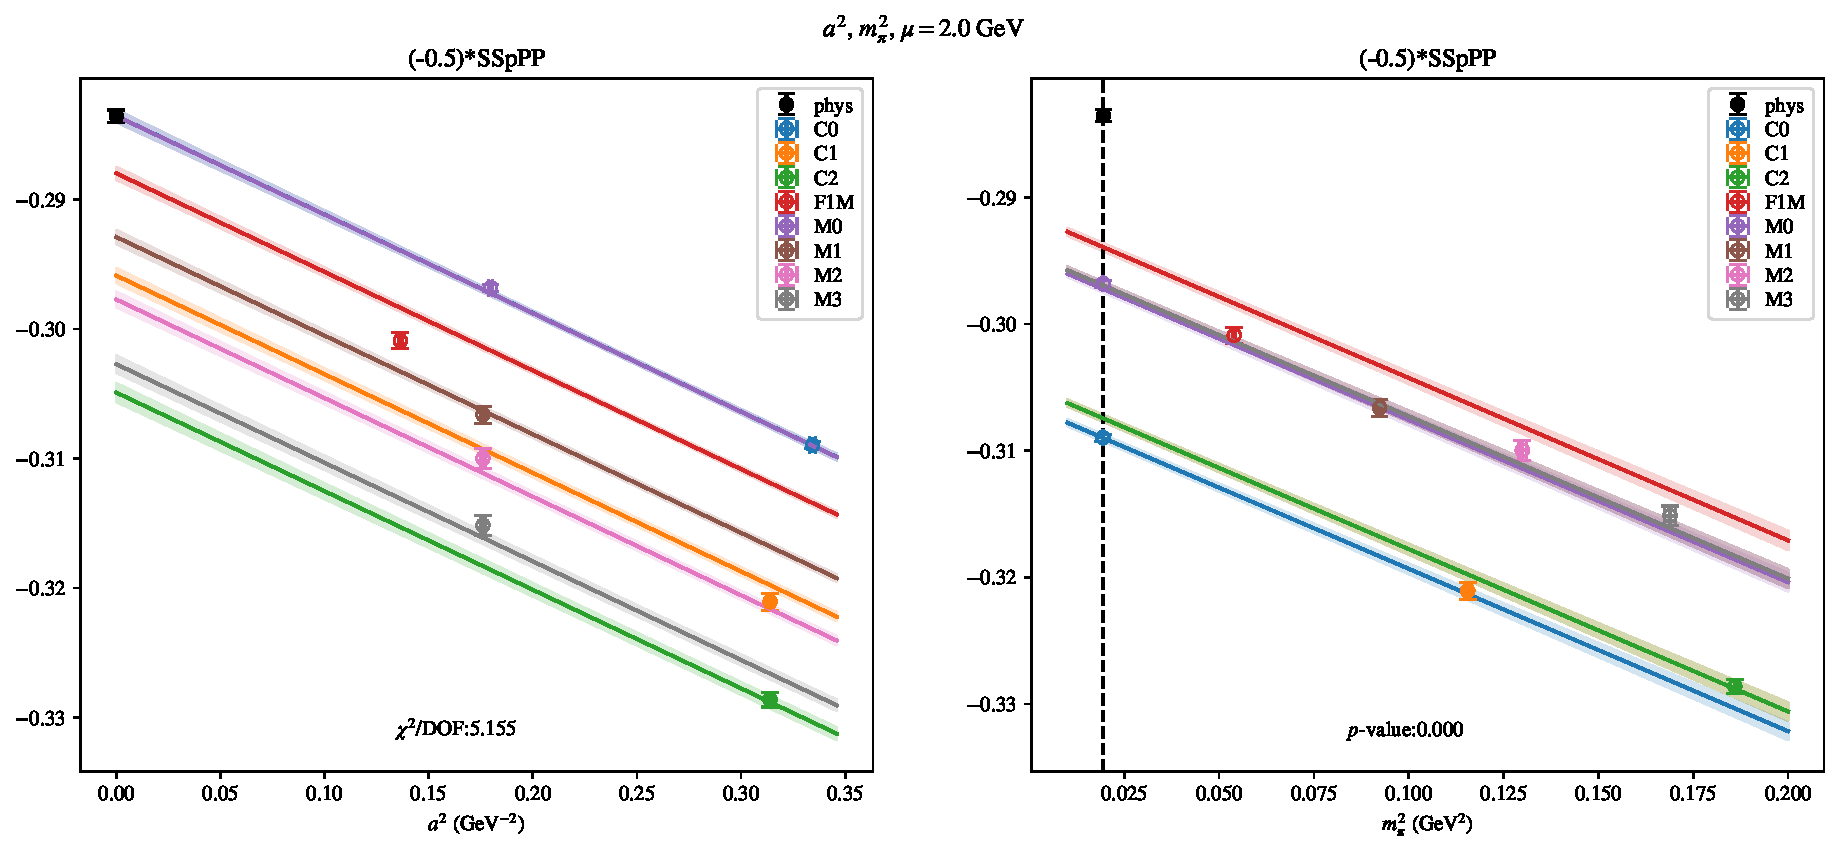
\includepdf[link, pages=-]{SSmPP/SUSY_F/a2m2_20.pdf}
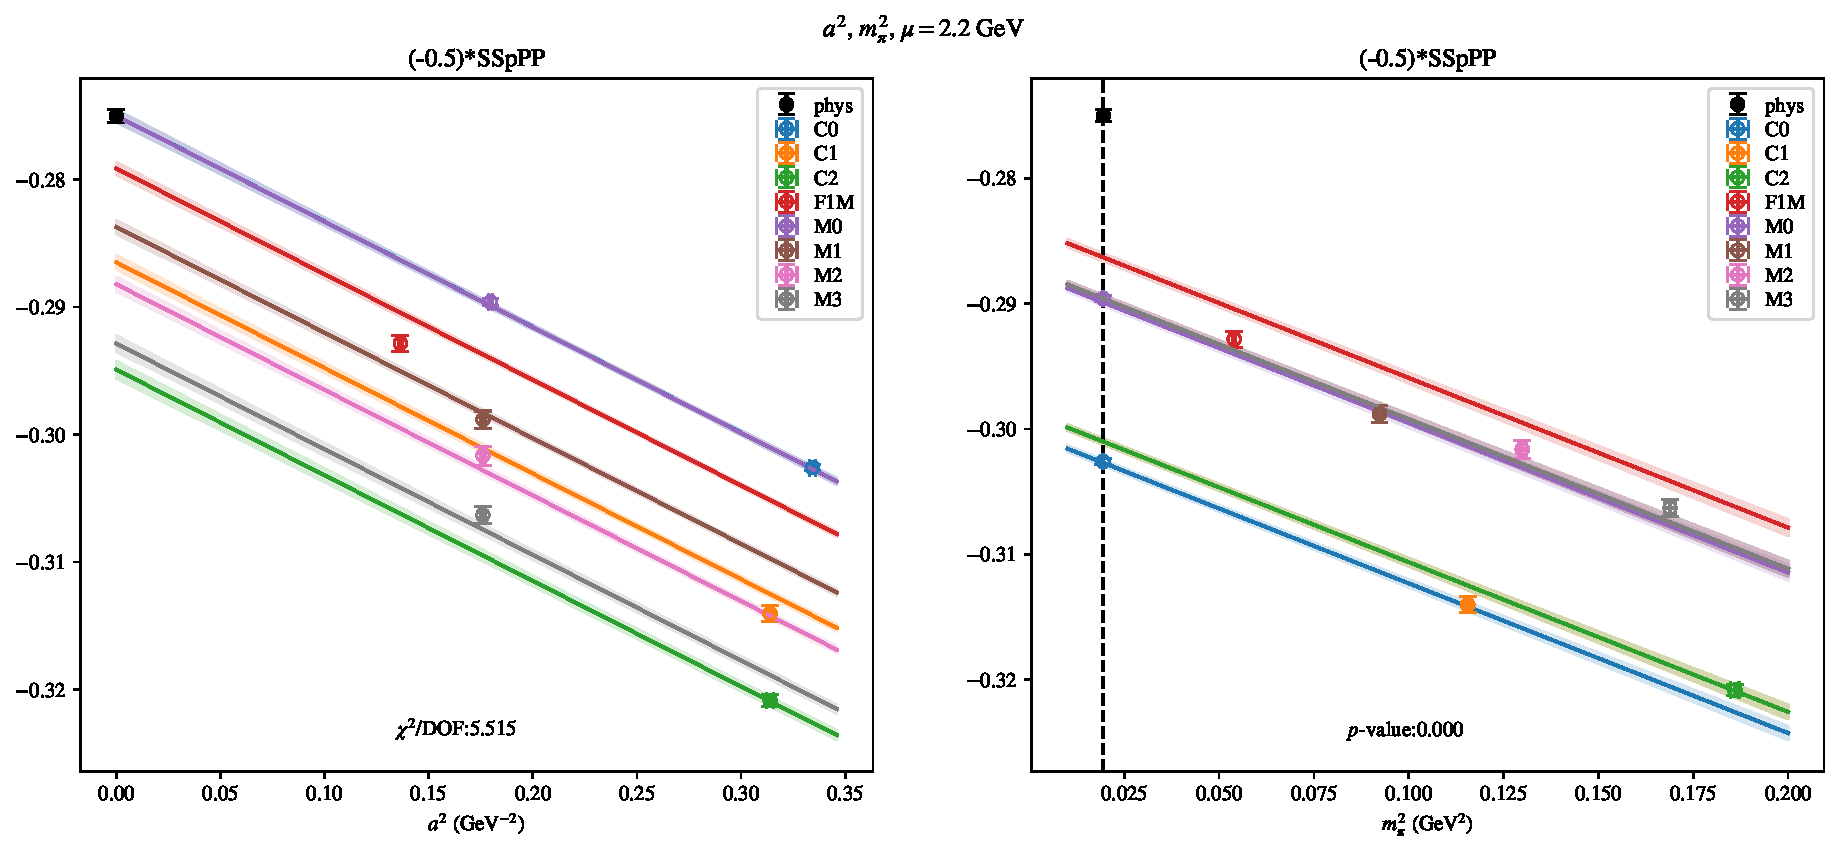
\includepdf[link, pages=-]{SSmPP/SUSY_F/a2m2_22.pdf}
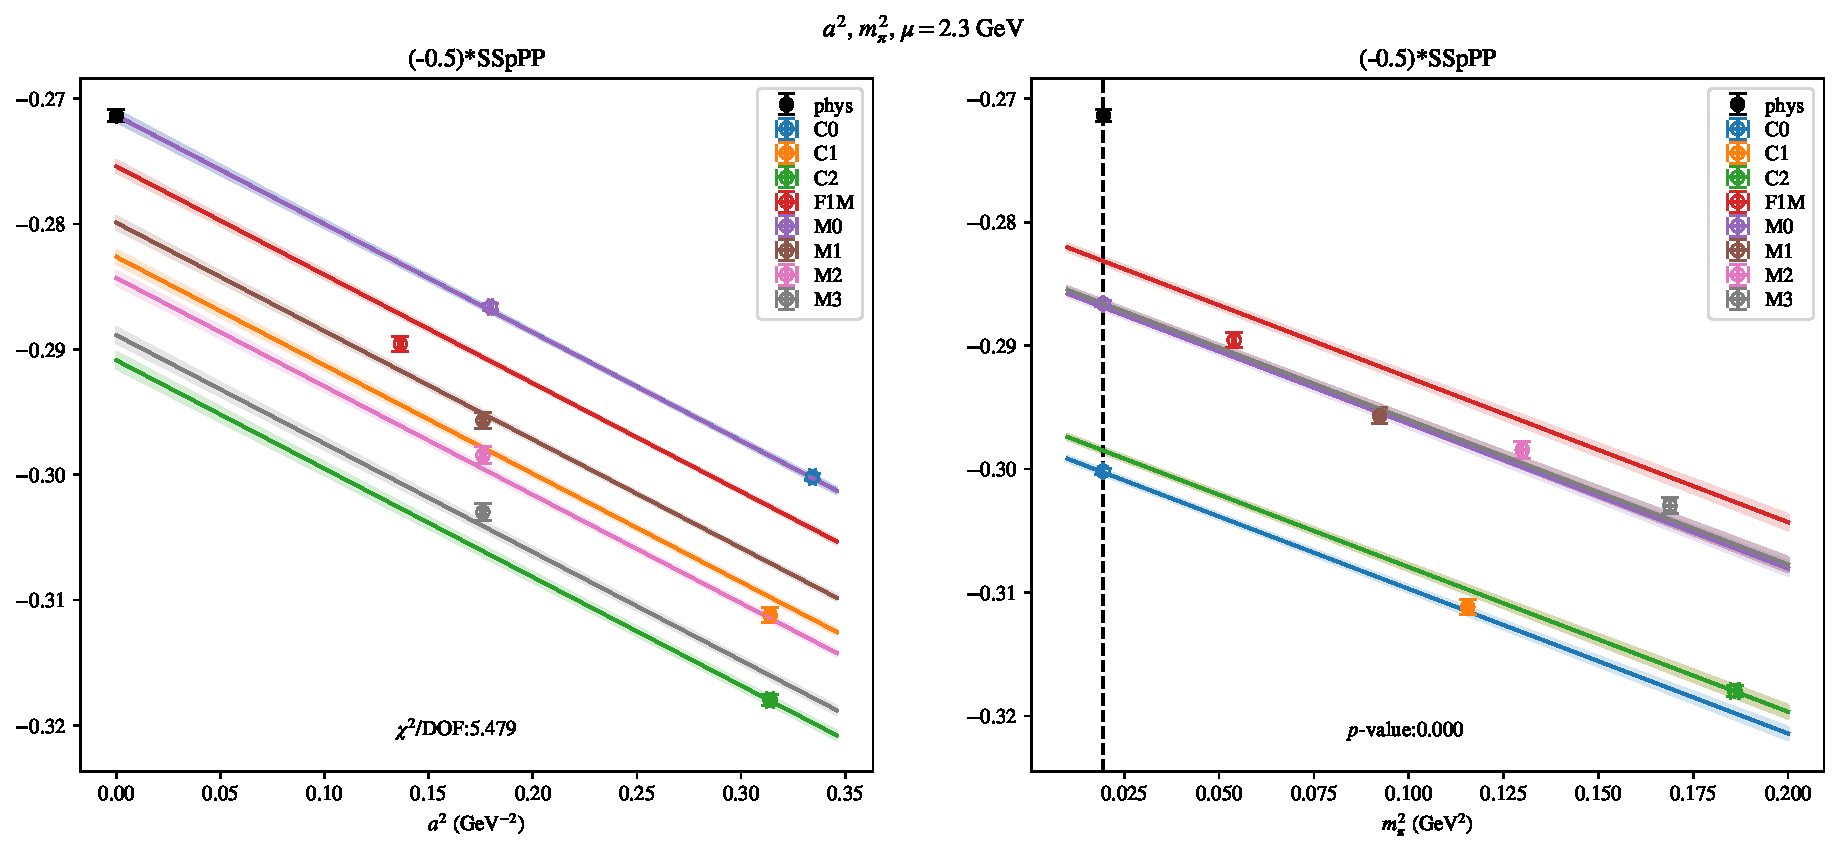
\includepdf[link, pages=-]{SSmPP/SUSY_F/a2m2_23.pdf}
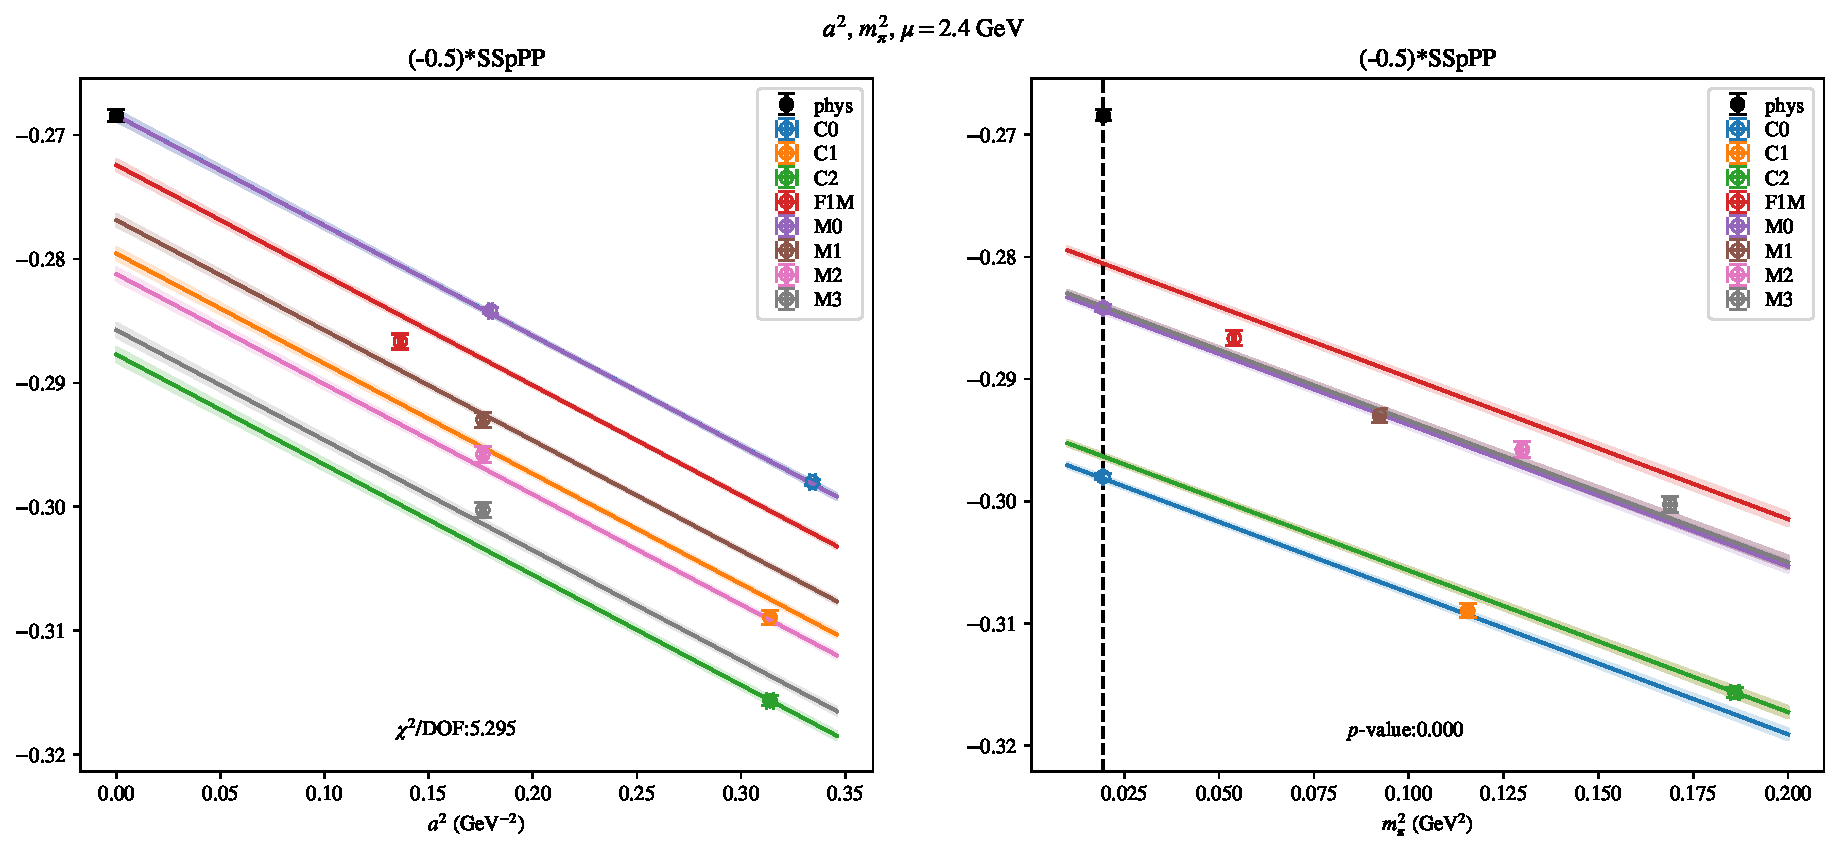
\includepdf[link, pages=-]{SSmPP/SUSY_F/a2m2_24.pdf}
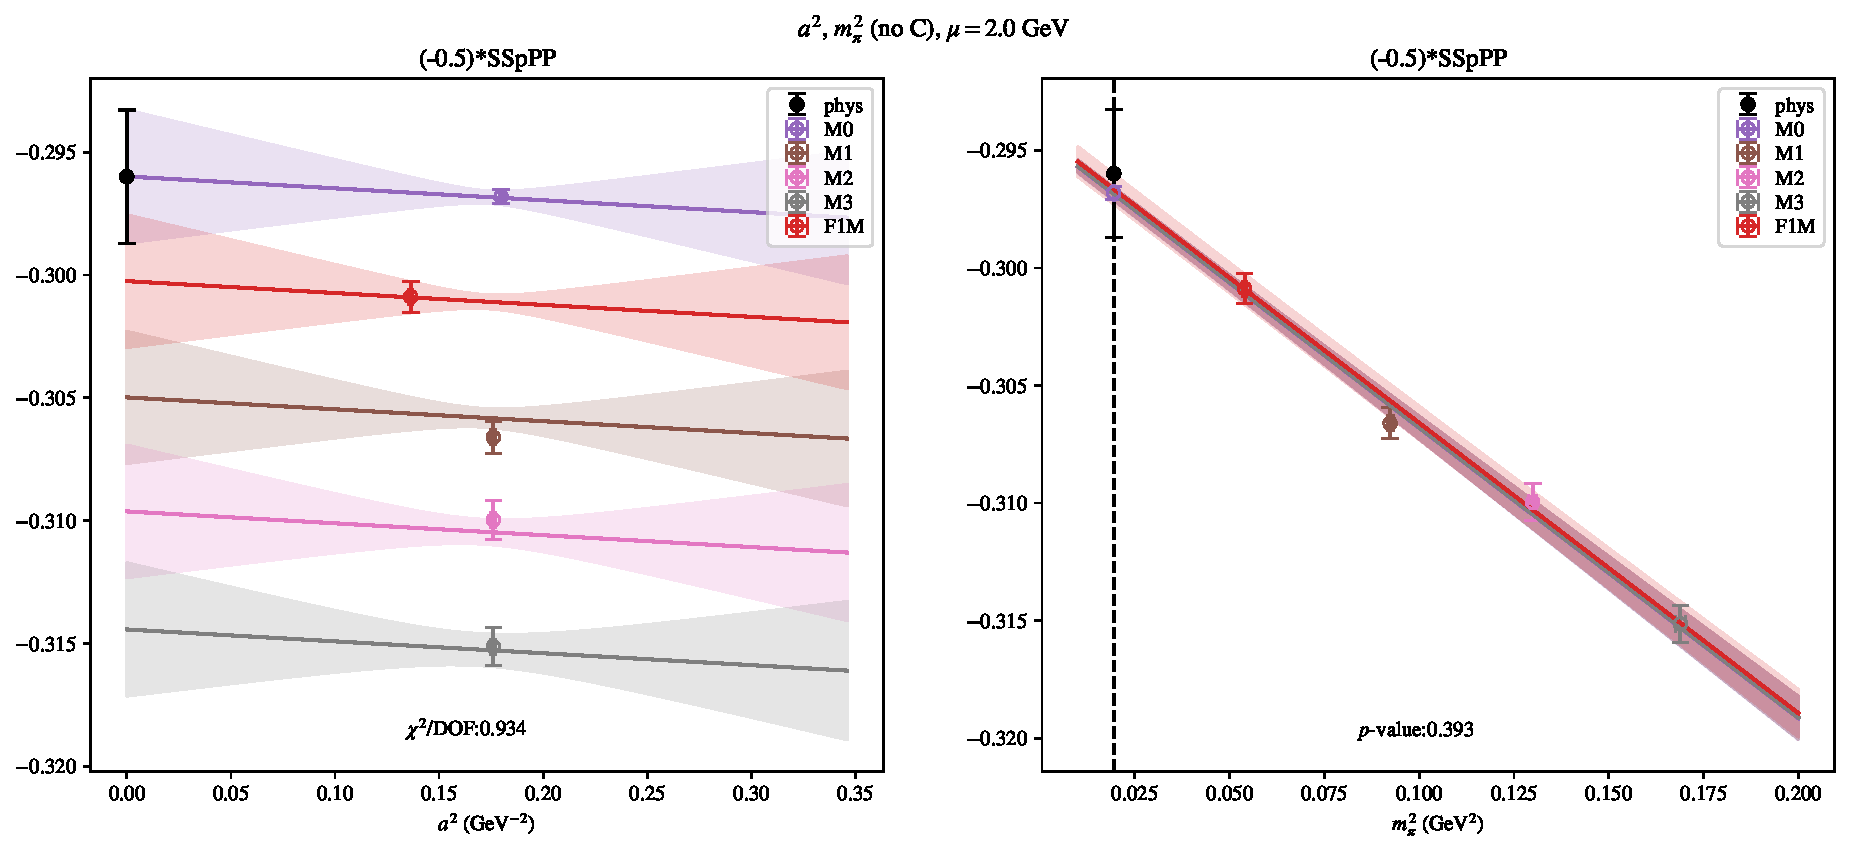
\includepdf[link, pages=-]{SSmPP/SUSY_F/a2m2noC_20.pdf}
\includepdf[link, pages=-]{SSmPP/SUSY_F/a2m2noC_22.pdf}
\includepdf[link, pages=-]{SSmPP/SUSY_F/a2m2noC_23.pdf}
\includepdf[link, pages=-]{SSmPP/SUSY_F/a2m2noC_24.pdf}
\includepdf[link, pages=-]{SSmPP/SUSY_F/a2a4m2_20.pdf}
\includepdf[link, pages=-]{SSmPP/SUSY_F/a2a4m2_22.pdf}
\includepdf[link, pages=-]{SSmPP/SUSY_F/a2a4m2_23.pdf}
\includepdf[link, pages=-]{SSmPP/SUSY_F/a2a4m2_24.pdf}
\includepdf[link, pages=-]{SSmPP/SUSY_F/a2m2mcut_20.pdf}
\includepdf[link, pages=-]{SSmPP/SUSY_F/a2m2mcut_22.pdf}
\includepdf[link, pages=-]{SSmPP/SUSY_F/a2m2mcut_23.pdf}
\includepdf[link, pages=-]{SSmPP/SUSY_F/a2m2mcut_24.pdf}
\includepdf[link, pages=-]{SSmPP/SUSY_F/a2m2m4_20.pdf}
\includepdf[link, pages=-]{SSmPP/SUSY_F/a2m2m4_22.pdf}
\includepdf[link, pages=-]{SSmPP/SUSY_F/a2m2m4_23.pdf}
\includepdf[link, pages=-]{SSmPP/SUSY_F/a2m2m4_24.pdf}
\clearpage
\section{$B_4$}
\begin{table}[h!]
\begin{center}
\begin{tabular}{|c|c|c|c|c|c|}
\hline
$\mu$ (GeV) & $a^2$, $m_\pi^2$& $a^2$, $m_\pi^2$ (no C)& $a^2$, $a^4$, $m_\pi^2$& $a^2$, $m_\pi^2$ (no M3, C2)& $a^2$, $m_\pi^2$, $m_\pi^4$\\
\hline
2.0& \hyperlink{SSpPP/SUSY_F/a2m2_20.pdf.1}{\textbf{-0.1856(54)}: 11.134 (0.0)} & \hyperlink{SSpPP/SUSY_F/a2m2noC_20.pdf.1}{\textbf{-0.172(16)}: 3.621 (0.027)} & \hyperlink{SSpPP/SUSY_F/a2a4m2_20.pdf.1}{\textbf{-0.162(26)}: 2.417 (0.046)} & \hyperlink{SSpPP/SUSY_F/a2m2mcut_20.pdf.1}{\textbf{-0.1856(62)}: 17.6 (0.0)} & \hyperlink{SSpPP/SUSY_F/a2m2m4_20.pdf.1}{\textbf{-0.1864(60)}: 12.06 (0.0)}\\
2.2& \hyperlink{SSpPP/SUSY_F/a2m2_22.pdf.1}{\textbf{-0.1937(48)}: 12.846 (0.0)} & \hyperlink{SSpPP/SUSY_F/a2m2noC_22.pdf.1}{\textbf{-0.179(15)}: 2.033 (0.131)} & \hyperlink{SSpPP/SUSY_F/a2a4m2_22.pdf.1}{\textbf{-0.169(25)}: 1.835 (0.119)} & \hyperlink{SSpPP/SUSY_F/a2m2mcut_22.pdf.1}{\textbf{-0.1936(56)}: 20.53 (0.0)} & \hyperlink{SSpPP/SUSY_F/a2m2m4_22.pdf.1}{\textbf{-0.1944(56)}: 14.51 (0.0)}\\
2.3& \hyperlink{SSpPP/SUSY_F/a2m2_23.pdf.1}{\textbf{-0.1972(47)}: 14.335 (0.0)} & \hyperlink{SSpPP/SUSY_F/a2m2noC_23.pdf.1}{\textbf{-0.182(15)}: 1.937 (0.144)} & \hyperlink{SSpPP/SUSY_F/a2a4m2_23.pdf.1}{\textbf{-0.172(25)}: 1.901 (0.107)} & \hyperlink{SSpPP/SUSY_F/a2m2mcut_23.pdf.1}{\textbf{-0.1972(53)}: 22.93 (0.0)} & \hyperlink{SSpPP/SUSY_F/a2m2m4_23.pdf.1}{\textbf{-0.1980(53)}: 15.537 (0.0)}\\
2.4& \hyperlink{SSpPP/SUSY_F/a2m2_24.pdf.1}{\textbf{-0.2002(48)}: 13.893 (0.0)} & \hyperlink{SSpPP/SUSY_F/a2m2noC_24.pdf.1}{\textbf{-0.185(15)}: 1.885 (0.152)} & \hyperlink{SSpPP/SUSY_F/a2a4m2_24.pdf.1}{\textbf{-0.175(25)}: 1.92 (0.104)} & \hyperlink{SSpPP/SUSY_F/a2m2mcut_24.pdf.1}{\textbf{-0.2002(54)}: 22.129 (0.0)} & \hyperlink{SSpPP/SUSY_F/a2m2m4_24.pdf.1}{\textbf{-0.2010(53)}: 14.939 (0.0)}\\
\hline
\end{tabular}
\caption{Physical point value from chiral and continuum extrapolation at renormalisation scale $\mu$. Entries are \textbf{value(error)}: $\chi^2/\text{DOF}$ ($p$-value).}
\end{center}
\end{table}
\begin{table}[h!]
\begin{center}
\begin{tabular}{|c c|c|c|c|c|c|}
\hline
$\mu$ (GeV) &  & $a^2$, $m_\pi^2$& $a^2$, $m_\pi^2$ (no C)& $a^2$, $a^4$, $m_\pi^2$& $a^2$, $m_\pi^2$ (no M3, C2)& $a^2$, $m_\pi^2$, $m_\pi^4$\\
\hline
\multirow{2}{0.5in}{2.0} & $\alpha$ & 0.7293(85)& 1.260(60)& 2.12(16)& 0.730(10)& 0.7140(99)\\
 & $\beta$ & -0.0021(13)& -0.0026(24)& -0.0031(18)& -0.0023(25)& -0.0045(76)\\
\hline
\multirow{2}{0.5in}{2.2} & $\alpha$ & 0.6667(75)& 1.192(57)& 2.05(16)& 0.6698(90)& 0.6537(91)\\
 & $\beta$ & -0.0022(13)& -0.0026(23)& -0.0032(17)& -0.0023(24)& -0.0043(75)\\
\hline
\multirow{2}{0.5in}{2.3} & $\alpha$ & 0.6414(74)& 1.173(55)& 2.05(15)& 0.6422(87)& 0.6265(87)\\
 & $\beta$ & -0.0022(13)& -0.0026(23)& -0.0031(17)& -0.0024(23)& -0.0047(72)\\
\hline
\multirow{2}{0.5in}{2.4} & $\alpha$ & 0.6244(74)& 1.136(54)& 1.97(15)& 0.6252(86)& 0.6097(86)\\
 & $\beta$ & -0.0021(13)& -0.0025(23)& -0.0031(17)& -0.0024(23)& -0.0047(71)\\
\hline
\end{tabular}
\caption{Fit values of coefficients in $B = B_{phys} + \mathbf{\alpha} a^2 + \mathbf{\beta}\left(\frac{m_\pi^2}{f_\pi^2}-\frac{m_{\pi,PDG}^2}{f_\pi^2}\right) + \ldots$.}
\end{center}
\end{table}
\includepdf[link, pages=-]{SSpPP/SUSY_F/a2m2_20.pdf}
\includepdf[link, pages=-]{SSpPP/SUSY_F/a2m2_22.pdf}
\includepdf[link, pages=-]{SSpPP/SUSY_F/a2m2_23.pdf}
\includepdf[link, pages=-]{SSpPP/SUSY_F/a2m2_24.pdf}
\includepdf[link, pages=-]{SSpPP/SUSY_F/a2m2noC_20.pdf}
\includepdf[link, pages=-]{SSpPP/SUSY_F/a2m2noC_22.pdf}
\includepdf[link, pages=-]{SSpPP/SUSY_F/a2m2noC_23.pdf}
\includepdf[link, pages=-]{SSpPP/SUSY_F/a2m2noC_24.pdf}
\includepdf[link, pages=-]{SSpPP/SUSY_F/a2a4m2_20.pdf}
\includepdf[link, pages=-]{SSpPP/SUSY_F/a2a4m2_22.pdf}
\includepdf[link, pages=-]{SSpPP/SUSY_F/a2a4m2_23.pdf}
\includepdf[link, pages=-]{SSpPP/SUSY_F/a2a4m2_24.pdf}
\includepdf[link, pages=-]{SSpPP/SUSY_F/a2m2mcut_20.pdf}
\includepdf[link, pages=-]{SSpPP/SUSY_F/a2m2mcut_22.pdf}
\includepdf[link, pages=-]{SSpPP/SUSY_F/a2m2mcut_23.pdf}
\includepdf[link, pages=-]{SSpPP/SUSY_F/a2m2mcut_24.pdf}
\includepdf[link, pages=-]{SSpPP/SUSY_F/a2m2m4_20.pdf}
\includepdf[link, pages=-]{SSpPP/SUSY_F/a2m2m4_22.pdf}
\includepdf[link, pages=-]{SSpPP/SUSY_F/a2m2m4_23.pdf}
\includepdf[link, pages=-]{SSpPP/SUSY_F/a2m2m4_24.pdf}
\clearpage
\section{$B_5$}
\begin{table}[h!]
\begin{center}
\begin{tabular}{|c|c|c|c|c|c|}
\hline
$\mu$ (GeV) & $a^2$, $m_\pi^2$& $a^2$, $m_\pi^2$ (no C)& $a^2$, $a^4$, $m_\pi^2$& $a^2$, $m_\pi^2$ (no M3, C2)& $a^2$, $m_\pi^2$, $m_\pi^4$\\
\hline
2.0& \hyperlink{TT/SUSY_F/a2m2_20.pdf.1}{\textbf{1.6418(22)}: 4.155 (0.001)} & \hyperlink{TT/SUSY_F/a2m2noC_20.pdf.1}{\textbf{1.598(11)}: 3.107 (0.045)} & \hyperlink{TT/SUSY_F/a2a4m2_20.pdf.1}{\textbf{1.574(18)}: 1.906 (0.106)} & \hyperlink{TT/SUSY_F/a2m2mcut_20.pdf.1}{\textbf{1.6422(24)}: 5.477 (0.001)} & \hyperlink{TT/SUSY_F/a2m2m4_20.pdf.1}{\textbf{1.6447(24)}: 3.403 (0.009)}\\
2.2& \hyperlink{TT/SUSY_F/a2m2_22.pdf.1}{\textbf{1.6266(22)}: 4.028 (0.001)} & \hyperlink{TT/SUSY_F/a2m2noC_22.pdf.1}{\textbf{1.581(11)}: 1.942 (0.143)} & \hyperlink{TT/SUSY_F/a2a4m2_22.pdf.1}{\textbf{1.554(18)}: 1.241 (0.291)} & \hyperlink{TT/SUSY_F/a2m2mcut_22.pdf.1}{\textbf{1.6270(24)}: 5.705 (0.001)} & \hyperlink{TT/SUSY_F/a2m2m4_22.pdf.1}{\textbf{1.6292(24)}: 3.625 (0.006)}\\
2.3& \hyperlink{TT/SUSY_F/a2m2_23.pdf.1}{\textbf{1.6203(22)}: 4.322 (0.001)} & \hyperlink{TT/SUSY_F/a2m2noC_23.pdf.1}{\textbf{1.573(11)}: 2.068 (0.126)} & \hyperlink{TT/SUSY_F/a2a4m2_23.pdf.1}{\textbf{1.546(17)}: 1.404 (0.23)} & \hyperlink{TT/SUSY_F/a2m2mcut_23.pdf.1}{\textbf{1.6207(23)}: 6.121 (0.0)} & \hyperlink{TT/SUSY_F/a2m2m4_23.pdf.1}{\textbf{1.6230(24)}: 3.83 (0.004)}\\
2.4& \hyperlink{TT/SUSY_F/a2m2_24.pdf.1}{\textbf{1.6154(22)}: 5.112 (0.0)} & \hyperlink{TT/SUSY_F/a2m2noC_24.pdf.1}{\textbf{1.565(11)}: 2.479 (0.084)} & \hyperlink{TT/SUSY_F/a2a4m2_24.pdf.1}{\textbf{1.536(17)}: 1.62 (0.166)} & \hyperlink{TT/SUSY_F/a2m2mcut_24.pdf.1}{\textbf{1.6160(23)}: 7.291 (0.0)} & \hyperlink{TT/SUSY_F/a2m2m4_24.pdf.1}{\textbf{1.6184(23)}: 4.508 (0.001)}\\
\hline
\end{tabular}
\caption{Physical point value from chiral and continuum extrapolation at renormalisation scale $\mu$. Entries are \textbf{value(error)}: $\chi^2/\text{DOF}$ ($p$-value).}
\end{center}
\end{table}
\begin{table}[h!]
\begin{center}
\begin{tabular}{|c c|c|c|c|c|c|}
\hline
$\mu$ (GeV) &  & $a^2$, $m_\pi^2$& $a^2$, $m_\pi^2$ (no C)& $a^2$, $a^4$, $m_\pi^2$& $a^2$, $m_\pi^2$ (no M3, C2)& $a^2$, $m_\pi^2$, $m_\pi^4$\\
\hline
\multirow{2}{0.5in}{2.0} & $\alpha$ & -0.019(51)& 0.136(42)& 0.36(10)& -0.020(57)& -0.025(56)\\
 & $\beta$ & 0.00032(13)& 0.00038(23)& 0.00021(14)& 0.0& -0.0014(63)\\
\hline
\multirow{2}{0.5in}{2.2} & $\alpha$ & -0.018(51)& 0.147(42)& 0.39(10)& -0.018(55)& -0.023(55)\\
 & $\beta$ & 0.0& 0.0& -0.0001(13)& -0.0002(23)& -0.0015(66)\\
\hline
\multirow{2}{0.5in}{2.3} & $\alpha$ & -0.016(51)& 0.154(42)& 0.40(10)& -0.016(55)& -0.021(55)\\
 & $\beta$ & -0.0& -0.0& -0.0002(13)& -0.0003(22)& -0.0016(64)\\
\hline
\multirow{2}{0.5in}{2.4} & $\alpha$ & -0.015(50)& 0.167(42)& 0.44(10)& -0.016(55)& -0.022(55)\\
 & $\beta$ & -0.0& -0.0& -0.0002(12)& -0.0003(20)& -0.0017(61)\\
\hline
\end{tabular}
\caption{Fit values of coefficients in $B = B_{phys} + \mathbf{\alpha} a^2 + \mathbf{\beta}\left(\frac{m_\pi^2}{f_\pi^2}-\frac{m_{\pi,PDG}^2}{f_\pi^2}\right) + \ldots$.}
\end{center}
\end{table}
\includepdf[link, pages=-]{TT/SUSY_F/a2m2_20.pdf}
\includepdf[link, pages=-]{TT/SUSY_F/a2m2_22.pdf}
\includepdf[link, pages=-]{TT/SUSY_F/a2m2_23.pdf}
\includepdf[link, pages=-]{TT/SUSY_F/a2m2_24.pdf}
\includepdf[link, pages=-]{TT/SUSY_F/a2m2noC_20.pdf}
\includepdf[link, pages=-]{TT/SUSY_F/a2m2noC_22.pdf}
\includepdf[link, pages=-]{TT/SUSY_F/a2m2noC_23.pdf}
\includepdf[link, pages=-]{TT/SUSY_F/a2m2noC_24.pdf}
\includepdf[link, pages=-]{TT/SUSY_F/a2a4m2_20.pdf}
\includepdf[link, pages=-]{TT/SUSY_F/a2a4m2_22.pdf}
\includepdf[link, pages=-]{TT/SUSY_F/a2a4m2_23.pdf}
\includepdf[link, pages=-]{TT/SUSY_F/a2a4m2_24.pdf}
\includepdf[link, pages=-]{TT/SUSY_F/a2m2mcut_20.pdf}
\includepdf[link, pages=-]{TT/SUSY_F/a2m2mcut_22.pdf}
\includepdf[link, pages=-]{TT/SUSY_F/a2m2mcut_23.pdf}
\includepdf[link, pages=-]{TT/SUSY_F/a2m2mcut_24.pdf}
\includepdf[link, pages=-]{TT/SUSY_F/a2m2m4_20.pdf}
\includepdf[link, pages=-]{TT/SUSY_F/a2m2m4_22.pdf}
\includepdf[link, pages=-]{TT/SUSY_F/a2m2m4_23.pdf}
\includepdf[link, pages=-]{TT/SUSY_F/a2m2m4_24.pdf}
\clearpage
\end{document}